\documentclass[MS]{wfuthesis}
\usepackage{tikz} % The GOAT
\usetikzlibrary{calc}
\usepackage{titlesec}
\usepackage[utf8]{inputenc}
\usepackage{graphicx} % Required for inserting images
\usepackage{subcaption} % Allows for the creation of subfigures
\usepackage{standalone} % Allows including standalone .tex files
\usepackage{multicol} % Multiple columns of text/figures
\usepackage{amsmath, amssymb} % Math packages
\usepackage{array}
\usepackage{booktabs}
\usepackage{hyperref}
\usepackage[capitalise]{cleveref}
\usepackage{xcolor} % Allows the creation of custom colors
\usepackage{algorithm, algpseudocode} % To write algorithm pseudo code
\usepackage{etoolbox}
\usepackage[intoc]{nomencl} % To add abbreviations page, intoc adds it to the table of contents
\usepackage{etoolbox} % goes with the above package, to add groupings to the abbreviations
\usepackage[backend=biber, natbib=true, style=numeric, sorting=none]{biblatex} % Bibliography and bibliography adjacent texts
\usepackage{xpatch}
\usepackage{nicefrac}
\usepackage{stmaryrd} 
\usepackage{pgfmath}
\usepackage{scalerel}
\usepackage{multirow}
\usepackage{xinttools}
\usepackage{pgfplots}
\usepgfplotslibrary{groupplots}


\title{\textbf{Advances in Tensor Decompositions: Fast Matrix Multiplication Algorithms And Parallel Adaptive Compression Techniques}}
\author{\textbf{João Victor de Oliveira Pinheiro}}
\date{May 2025}
\linespread{1.5}

\department{Computer Science}
\advisor{Grey Ballard, Ph.D.}
\chairperson{Aditya Devarakonda, Ph.D.}
\member{Frank Moore, Ph.D.}
\member{Ramakrishnan Kannan, Ph.D.}

\newcommand{\JP}[1]{\textcolor{purple}{\textbf{JP:} #1}}
\newcommand{\GB}[1]{\textcolor{red}{\textbf{GB:} #1}}
\newcommand{\AD}[1]{\textcolor{blue}{\textbf{AD:} #1}}
\newcommand{\FM}[1]{\textcolor{green}{\textbf{FM:} #1}}
\newcommand{\RK}[1]{\textcolor{orange}{\textbf{RK:} #1}}



%%%%%%%%%%%%%%%%%%%%%%%%%
%% My Own Shennenigans %%
%%%%%%%%%%%%%%%%%%%%%%%%%

\titleformat{\chapter}[display]
  {\bfseries\Large}  % Format for the chapter title
  {}                 % No "Chapter X" label
  {0pt}              % Space between number and title
  {\Large}           % Additional formatting for the title

\definecolor{mycustomgreen}{RGB}{44, 183, 66}
\definecolor{mycustomorange}{RGB}{255, 149, 1}
\definecolor{mycustompurple}{RGB}{181, 29, 227}

\makenomenclature
\renewcommand{\nomname}{\textbf{LIST OF ABREVIATIONS}}
\renewcommand\nomgroup[1]{%
  \item[\bfseries
  \ifstrequal{#1}{C}{CP Decompositions}{}%
  \ifstrequal{#1}{T}{Tucker Decompositions}{}%
]}

\algrenewcommand\alglinenumber[1]{{\sffamily\footnotesize#1}}

\makeatletter
\xpatchcmd{\algorithmic}{\itemsep\z@}{\itemsep=-1.5ex}{}{}
\makeatother

\addbibresource{references.bib}



%%%%%%%%%%%%
%% THESIS %%
%%%%%%%%%%%%

\begin{document}
    
\usetikzlibrary{3d,calc}

%% ------------------------------------------------------------
%% MACROS
%% ------------------------------------------------------------


%% --- Extras ---
% Transpose
\newcommand{\Tra}{{\sf T}} 
\newcommand{\parens}[1]{(#1)}
\newcommand{\Parens}[1]{\left(#1\right)}
\newcommand{\dsquare}[1]{\llbracket #1 \rrbracket}
\newcommand{\Dsquare}[1]{\left\llbracket #1 \right\rrbracket}
\newcommand{\curly}[1]{\{ #1 \}}
\newcommand{\Curly}[1]{\left\{ #1 \right\}}
\newcommand{\Real}{\mathbb{R}}
\newcommand{\qtext}[1]{\quad\text{#1}\quad}
\newcommand{\iddots}{\scalebox{-1}[1]{$\ddots$}}
\newcommand{\plusequals}{\mathrel{+}=}

%% --- Vectors ---
% vector
\newcommand{\V}[2][]{{\bm{#1\mathbf{\MakeLowercase{#2}}}}} 
% element of vector
\newcommand{\VE}[3][]{#1{\MakeLowercase{#2}}_{#3}} 
% vector in series
\newcommand{\Vn}[3][]{{\bm{#1\mathbf{\MakeLowercase{#2}}}}^{(#3)}} 
% transposed vector in series
\newcommand{\VnTra}[3][]{{\bm{#1\mathbf{\MakeLowercase{#2}}}}^{(#3)\Tra}} 
% element of vector in series
\newcommand{\VnE}[4][]{#1{\MakeLowercase{#2}}^{(#3)}_{#4}} 

%% --- Matrices ---
% matrix
\newcommand{\M}[2][]{{\bm{#1\mathbf{\MakeUppercase{#2}}}}} 
% matrix in series
\newcommand{\Mn}[3][]{{\bm{#1\mathbf{\MakeUppercase{#2}}}}^{(#3)}} 
% transposed matrix in series 
\newcommand{\MnTra}[4][]{{\bm{#1\mathbf{\MakeUppercase{#2}}}}^{(#3)\Tra}} 
% matrix column
\newcommand{\MC}[3][]{\V[#1]{#2}_{#3}} 
% column of matrix in series
\newcommand{\MnC}[4][]{\Vn[#1]{#2}{#3}_{#4}} 
% transposed column of matrix in series
\newcommand{\MnCTra}[4][]{\VnTra[#1]{#2}{#3}_{#4}} 
% matrix element
\newcommand{\ME}[3][]{#1{\MakeLowercase{#2}}_{#3}} 
% element of matrix in series
\newcommand{\MnE}[4][]{#1{\MakeLowercase{#2}}^{(#3)}_{#4}} 

%% --- Tensors ---
% tensor
\newcommand{\T}[2][]{\boldsymbol{#1\mathscr{\MakeUppercase{#2}}}} 
% tensor slide
\newcommand{\TS}[3][]{\M[#1]{#2}_{#3}}
% tensor element
\newcommand{\TE}[3][]{#1{\MakeLowercase{#2}}_{#3}}
% matriczied tensor
\newcommand{\Mz}[3][]{\M[#1]{#2}_{(#3)}}
% tensor in series
\newcommand{\Tn}[3][]{{\boldsymbol{#1\mathscr{\MakeUppercase{#2}}}}^{(#3)}} 
% matricized tensor in series
\newcommand{\Mzn}[4][]{#1\mathbf{\MakeUppercase{#2}}^{(#3)}_{(#4)}}

%% --- Operators ---
% outer product
\newcommand{\Oprod}{\circ} 
% Kronecker product
\newcommand{\Kron}{\otimes} 
% Khatri-Rao product
\newcommand{\Khat}{\odot} 
% Hadamard (elementwise multiply)
\newcommand{\Hada}{\ast} 
\newcommand{\BigHada}{\mathop{\mbox{\fontsize{18}{19}\selectfont $\circledast$}}} 
% Elementwise divide
\newcommand{\Divi}{\varoslash}

\newcommand{\GB}[1]{{\color{blue}\textbf{GB:}~#1}}
\newcommand{\ignore}[1]{}
    \maketitle
    %%%%%%%%%%%%%%%%%%%%%%
    %% Acknowledgements %%
    %%%%%%%%%%%%%%%%%%%%%%
    \section*{\textbf{ACKNOWLEDGEMENTS}} 
        Dedico este trabalho aos meus pais, que sob muito sol, fizeram-me chegar até aqui, na sombra.
        
        % To all of those that came before me, and to all of those who are yet to come

        % I would like to thank the Whitener family. Specifically the trouble child that is Nathan

        % I would like to thank Joe and Gabby not because they are physicis (boo)
        % but because they are kinda cool





    %%%%%%%%%%%%%%%%%%%%%%%
    %% Table of Contents %%
    %%%%%%%%%%%%%%%%%%%%%%%
    \tableofcontents
    \newpage





    %%%%%%%%%%%%%%%%%%%%%%%%%%%
    %% List of Illustrations %%
    %%%%%%%%%%%%%%%%%%%%%%%%%%%
    \listoffigures
    \newpage





    %%%%%%%%%%%%%%%%%%%%%%%%%%
    %% List of Abreviations %%
    %%%%%%%%%%%%%%%%%%%%%%%%%%
    \nomenclature[C]{CP:}{Cynical Polynomial}
    \nomenclature[T]{LLSV:}{Left Leading Singular Values}
    \nomenclature[T]{EVD:}{Eigenvalue Decomposition}
    \nomenclature[T]{SVD:}{Singular Value Decomposition}
    \nomenclature[T]{HOSVD:}{Higher Order Singular Value Decomposition}
    \nomenclature[T]{STHOSVD:}{Sequentially Truncated Higher Order Singular Value Decomposition}
    \nomenclature[T]{HOOI:}{Higher Order Orthogonal Iterations}
    \nomenclature[T]{HOSI:}{Higher Order Subspace Iterations}
    \nomenclature[T]{DT:}{Dimention Trees}

    \printnomenclature
    \newpage





    %%%%%%%%%%%%%%
    %% Abstract %%
    %%%%%%%%%%%%%%
    \addcontentsline{toc}{chapter}{\textbf{ABSTRACT}}
    \begin{center}
        \textbf{ABSTRACT}
    \end{center}
    Tensors are essential in modern-day computational and data sciences. This
    work presents recent advances in tensor decompositions which are techniques
    that break down complex high-dimensional arrays into smaller structured
    components. There are two projects presented in this thesis, each in its own
    abstract and chapter. 
    % The first project applies tensor decompositions on searches for new
    % algorithms for fast matrix multiplication. The second project focuses on the
    % development of scalable, adaptive methods for compressing massive data sets.

    \textbf{Searching For Fast Matrix Multiply Algorithms using Cyclic-Invariant
    CP decomposition:} Fast matrix multiplication algorithms correspond to exact
    CP decompositions of tensors that encode matrix multiplication of fixed
    dimensions. This 3-way matrix multiplication tensor has cyclic symmetry: the
    entry values are invariant under cyclic permutation of the indices. The CP
    decomposition of Strassen's original fast matrix multiplication algorithm
    for 2x2 matrices is cyclic invariant, which means a cyclic permutation of
    the CP factors results in the same CP components, just in a different order.
    We describe how to search for these solutions, using the damped Gauss-Newton
    optimization method along with heuristic rounding techniques. We not only
    summarize the algorithms discovered so far but also attempt to search for
    further structure in these algorithms; the $GL_3$ and the transpose-like
    symmetry. After discussing what algorithms require to have such structure,
    we describe how future work can modify our search algorithm further to
    obtain solutions with all three structure.
    
    % are known to exist for 3x3 and 4x4 matrix multiplication as well. 


    \textbf{Parallel Higher-Order Orthogonal Iteration for Tucker Decomposition
    with Rank Adaptivity:} Higher Order Orthogonal Iteration (HOOI) is an
    algorithm that uses block coordinate descent optimization to compress an
    input tensor into a Tucker format approximation. Classical HOOI requires
    specifying the ranks, or dimensions of the core tensor, and seeks to
    minimize the approximation error. 	We introduce HOOI-Adapt, a novel
    error-specified algorithm that adaptively selects the ranks of the Tucker
    tensor in order to maximize the compression subject to the error threshold.
    We implement HOOI-Adapt using the distributed-memory parallel TuckerMPI
    library and employ memoization to reduce the computational cost.
    Furthermore, we show that when the ranks are small, HOOI-Adapt has lower
    computational cost compared to the alternative Sequentially Truncated
    Higher-Order SVD (ST-HOSVD) algorithm. Our benchmarks demonstrate that our
    parallel implementation of HOOI-Adapt outperforms TuckerMPI's ST-HOSVD for
    small ranks when scaled to terabyte-sized input datasets on NERSC's
    Perlmutter platform.





    %%%%%%%%%%%%%%%%%%
    %% Introduction %%
    %%%%%%%%%%%%%%%%%%
    \chapters{}
    \chapter{\textbf{Introduction}}
        %!TEX root = ../../main.tex

\section{Tensor and Their Subparts} \label{sec:Tensor and Their Subparts}
    %!TEX root = ../../main.tex

\subsection{What Is A Tensor?} \label{sec:What is A Tensor} There is no widely
    agreed definition of a tensor; different fields define it differently. For
    the purposes of this work, we define tensors through the definition widely
    used in the field of computer science. A \textbf{tensor} is a $d$-way
    array, where $d$ is referred to as the order of the tensor. Before we move
    on any further, a bit of notation is required. The set of real values is
    denoted as $\mathbb{R}$. Letters $m, n, p, q, r$ are used to represent sizes
    (or simply $n_1, \cdots, n_d$) and letters $i, j, k, \ell$ are used to
    represent indices (or simply $i_1, \cdots, i_d$). For the sake of
    simplification, let $[n] \equiv [1, \cdots, n]$, and furthermore let $[m]
    \otimes [n] \equiv \{ (i, j) | i\in[m], j\in[n]\}$. Some lower order tensors
    have other names:


    \begin{itemize}
        \item A \textbf{scalar} is a `zero-dimensional' tensor. This is any
        number $x\in \mathbb{R}$. 
        \item A \textbf{vector} is a one-dimensional array of scalars that
        represent a collection of measurements. This can be visualzied on Figure
        \ref{fig:vector}. We represent vectors by lowercase boldface roman
        letters. If $\mathbf{x}$ is a real-valued vector of size $n$, then we
        write that $\mathbf{x} \in \mathbb{R}^n$. Entry $i\in [n]$ of
        $\mathbf{x}$ is denoted as $\mathbf{x}(i)$, or compactly as
        $\mathbf{x}_i$. A vector is a tensor of order 1. Instead of referring to
        them as order 1 tensors, they will simply be referred to as vectors. 
        \item A \textbf{matrix} is a two-dimensional array of numbers, such
        as a collection of vectors This can be vizualized on Figure
        \ref{fig:matrix}. We represent matrices by uppercase boldface roman
        letters. If $\mathbf{X}$ is a real-valued matrix of size $m\times
        n$, then we write $\mathbf{X}\in \mathbb{R}^{m\times n}$. The matrix
        entry $\mathbf{X}(i, j)$ woud represent the $i^\text{th}$ entry of
        vector $j$. More generally, entry $(i, j)\in [m] \otimes [n]$ of
        $\mathbf{X}$ is denoted as $X(i, j)$ or compactly as $\mathbf{x}_{i,
        j}$. A matrix is a tensor of order 2. Instead of referring to
        them as order 2 tensors, they will simply be referred to as matrices.
    \end{itemize}


    \begin{figure}[ht]
        \def\distance{0.2}
        \def\one{0.3}
        \def\n{2}
        \def\m{2.5}
        \def\p{1.5}
        \def\rot{90}

        \centering
        
        % First Subfigure
        \begin{subfigure}[b]{0.26\textwidth}
            \centering
            \begin{tikzpicture}[namenode/.style={scale=1}]

    \coordinate (v) at (0, 0);
    \coordinate (center_v) at ($(\one/2, \n/2)$);

    \coordinate (n_arrow) at ($(v) + (-\distance, \n)$);
    \coordinate (n) at ($(n_arrow) + (-1.25*\distance, -\n/2)$);
    
    \coordinate (one_arrow) at ($(v) + (0, -\distance)$);
    \coordinate (one) at ($(center_v) + (0, -7.5*\distance)$);
    
    \draw[] (v) rectangle (\one, \n);
    \node[namenode] at (center_v) {$\mathbf{x}$};

    \draw[->] (n_arrow) -- (-\distance, 0);
    \node[namenode] at (n) {$n$};
    
    \draw[->] (one_arrow) -- (\one, -\distance);
    \node[namenode] at (one) {$1$};

\end{tikzpicture}x=
            \caption[a Vector]{Vector $\mathbf{x}\in \mathbb{R}^n$ is a 1-way tensor}
            \label{fig:vector}
        \end{subfigure}
        \hfill
        % Second Subfigure
        \begin{subfigure}[b]{0.3\textwidth}
            \centering
            \begin{tikzpicture}[namenode/.style={scale=1}]

    \coordinate (M) at (0, 0);
    \coordinate (center_M) at ($(\m/2, \n/2)$);

    \coordinate (n_arrow) at ($(M) + (-\distance, \n)$);
    \coordinate (n) at ($(n_arrow) + (-1.25*\distance, -\n/2)$);
    
    \coordinate (m_arrow) at ($(M) + (0, -\distance)$);
    \coordinate (m) at ($(center_M) + (0, -7.5*\distance)$);
    
    \draw[] (M) rectangle (\m, \n);
    \node[namenode] at (center_M) {$\mathbf{X}$};

    \draw[->] (n_arrow) -- (-\distance, 0);
    \node[namenode] at (n) {$m$};
    
    \draw[->] (m_arrow) -- (\m, -\distance);
    \node[namenode] at (m) {$n$};

\end{tikzpicture}
            \caption[a Matrix]{Matrix $\mathbf{X} \in \mathbb{R}^{m\times n}$ is a 2-way tensor}
            \label{fig:matrix}
        \end{subfigure}
        \hfill
        % Third Subfigure
        \begin{subfigure}[b]{0.31\textwidth}
            \centering
            \begin{tikzpicture}[namenode/.style={scale=1}]

    \coordinate (M) at (0, 0);
    \coordinate (center_M) at ($(\m/2, \n/2)$);

    \coordinate (n_arrow) at ($(M) + (-\distance, \n)$);
    \coordinate (n) at ($(n_arrow) + (-1.25*\distance, -\n/2)$);
    
    \coordinate (m_arrow) at ($(M) + (0, -\distance)$);
    \coordinate (m) at ($(center_M) + (0, -7.5*\distance)$);
    
    \draw[] (M) rectangle (\m, \n);
    \node[namenode] at (center_M) {$\mathcal{X}$};

    % This scope draws the top face of the cube
    \begin{scope}[shift={(M)}, canvas is zx plane at y=\n,rotate=\rot]
        \draw (0,0) rectangle (\m,\p);
    \end{scope}
    
        % This scope draws the left side of the cube
    \begin{scope}[shift={(M)},canvas is zy plane at x=\m,rotate=90]
        \draw (0,0) rectangle (\n,\p); %
    \end{scope}
    
    \draw[->] (n_arrow) -- (-\distance, 0);
    \node[namenode] at (n) {$m$};
    
    \draw[->] (m_arrow) -- (\m, -\distance);
    \node[namenode] at (m) {$n$};

    \coordinate (p_arrow) at ($(n_arrow) + (\distance, \distance)$);
    \coordinate (p_arrow_end) at ($(p_arrow) + (0.3*\p, 0.3*\p)$);
    \coordinate (p) at (0, 2.5);
    \draw[->] (p_arrow) -- (p_arrow_end);
    \node[namenode] at (p) {$p$};

\end{tikzpicture}
            \caption[a 3D Tensor]{Tensor $\mathcal{X}\in \mathbb{R}^{m\times n \times p}$ is a 3-way tensor}
            \label{fig:tensor3}
        \end{subfigure}

        % Main Figure Caption
        \caption{Tensors of orders one, two, and three}
        \label{fig:Tensors123}
    \end{figure}

    If we have a three-dimensional array of numners, then we have a higher-order
    tensor. Tensors of order 3 or greater are denoted by uppercase mathematical
    caligraphy letters: $\mathcal{X}$. This can be vizualized on
    \Cref{fig:tensor3}. If $\mathcal{X}$ is a real-valued tensor of size
    $m\times n \times p$, then we write $\mathcal{X}\in \mathbb{R}^{m\times
    n\times p}$. For instance, given a set of $m$ objects, each of which has $n$
    features, measured under $p$ different scenatios, the tensor entry
    $\mathcal{X}(i, j, k)$ would represent the $j^\text{th}$ feature of object
    $i$ measured in scenario $k$. More generally, entry $(i, j, k) \in
    [m]\otimes [n]\otimes [p]$ of $\mathcal{X}$ is denoted as $X(i, j, k)$ or
    compactly as $x_{i, j, k}$. We refer to each dimension as a \textbf{mode}.
    Of a 3-way tensor, we say that mode 1 is of size $m$, mode 2 of size $n$,
    and mode 3 of size $p$. If all modes have the same size, we call this tensor
    \textbf{uniform}.

    As mentioned earlier, any tensor of order greater or equal to three is
    simply referred to as a higher-order tensor. But we begin to run out of
    letters to describe its size and index its modes. This is when we resort
    to subscripts mentioned earlier. \Cref{fig:Tensors45} illustrate
    4-way and 5-way tensors. There, we can visualize the recursive nature of
    tensors. A 4-way tensor is really an array of 3-way tensors, in real
    life that is often used to describe an experiment with three spatial
    dimensions and one time dimension. Similarly, a 5-way tensor is really a
    martrix of 3-way tensors, in real life that is often used to describe an
    experiment with 3 spatial dimensions, one time dimension, and and a
    certain amount of variables being measured is the fifth fimension. To
    remember all of this, \Cref{tab:tensor_notation}

    % Define a command to draw a single cube
    \newcommand{\drawcube}[1]{
        % These distances can be meddled with to get you what you want
        \def\ix{2} %
        \def\iy{2} %
        \def\iz{1.5} %
        \def\corescale{1}
        \def\rot{90}
        \def\r{0.25} % Thickness of edges
        \def\rx{\ix/\corescale}
        \def\ry{\iy/\corescale}
        \def\rz{\iz/\corescale}

        % Draw the cube
        \begin{tikzpicture}[scale=#1, every node/.style={inner sep=0pt}] % Scale for smaller cubes
            % Define starting point
            \coordinate (TFrontLowerLeft) at (0,0);
            \draw (TFrontLowerLeft) rectangle ++ (\rx,\ry); % Front face

            % Top face
            \begin{scope}[shift={(TFrontLowerLeft)}, canvas is zx plane at y=\ry,rotate=\rot]
            \draw (0,0) rectangle ++ (\rx,\rz);
            \end{scope}

            % Left face
            \begin{scope}[shift={(TFrontLowerLeft)},canvas is zy plane at x=\rx,rotate=\rot]
            \draw (0,0) rectangle ++ (\ry,\rz);
            \end{scope}
        \end{tikzpicture}
    }

    \begin{figure}[ht]
        \centering
        
        % First Subfigure
        \begin{subfigure}[b]{0.49\textwidth}
            \centering
            \[
                \left[
                \begin{array}{c}
                    \drawcube{0.4} \\
                    \vdots \\
                    \drawcube{0.4}
                \end{array}
                \right]
            \]     
            \caption[a 4D Tensor]{A 4D Tensor \newline $\mathcal{X}\in \mathbb{R}^{n_1\times n_2 \times n_3 \times n_4}$}
            \label{fig:tensor4}
        \end{subfigure}
        \hfill
        % Second Subfigure
        \begin{subfigure}[b]{0.49\textwidth}
            \centering
            \[
                \left[
                \begin{array}{ccc}
                    \drawcube{0.4} & \hdots & \drawcube{0.4} \\
                    \vdots & \ddots & \vdots \\
                    \drawcube{0.4} & \hdots & \drawcube{0.4}
                \end{array}
                \right]
            \]
            \caption[a 5D Tensor]{A 5D Tensor \newline $\mathcal{X}\in \mathbb{R}^{n_1\times n_2 \times n_3 \times n_4 \times n_5}$}
            \label{fig:tensor5}
        \end{subfigure}

        % Main Figure Caption
        \caption{Tensors of orders four and five}
        \label{fig:Tensors45}
    \end{figure}

    \begin{table}[ht!]
        \centering
        \renewcommand{\arraystretch}{0.5}
        \begin{tabular}{@{}llcll@{}}
        \toprule
        \textbf{Description} & \textbf{Size} & \textbf{Order} & \textbf{Notation} & \textbf{Entry} \\ 
        \midrule
        Scalar         & $1$                         & $0$ & $x$        & $x$ \\
        Vector         & $n$                         & $1$ & $\mathbf{x}$        & $x(i)$ or $x_i$ \\
        Matrix         & $m \times n$                & $2$ & $\mathbf{X}$        & $X(i,j)$ or $x_{ij}$ \\
        3-way tensor   & $m \times n \times p$       & $3$ & $\mathcal{X}$       & $X(i,j,k)$ or $x_{ijk}$ \\
        4-way tensor   & $n_1 \times n_2 \times n_3 \times n_4$ & $4$ & $\mathcal{X}$ & $X(i_1,i_2,i_3,i_4)$ or $x_{i_1i_2i_3i_4}$ \\
        $d$-way tensor & $n_1 \times n_2 \times \cdots \times n_d$ & $d$ & $\mathcal{X}$ & $X(i_1, i_2, \dots, i_d)$ or $x_{i_1i_2\cdots i_d}$ \\
        \bottomrule
        \end{tabular}
        \caption{Tensor Notation by Order}
        \label{tab:tensor_notation}
    \end{table}

\subsection{Slices and Fibers} \label{sec:Slices and Fibers}
    A slice of a 3-way tensor $\mathcal{X}\in\mathbb{R}^{m\times n\times p}$ is
    a 2-way subtensor (which is a matrix). The $i^\text{th}$ \textbf{horizontal
    slice} is a matrix of size $n \times p$ given by $\mathcal{X}(i, :, :)$. The
    $j^\text{th}$ \textbf{lateral slice} is a matrix of size $m\times n$ given
    by $\mathcal{X}(:, j, :)$. The $k^\text{th}$ \textbf{frontal slice} is a
    matrix of size $m\times n$ given by $\mathcal{X}(:, :, k)$. The three types
    of slices for 3-way tensors are shown in \Cref{fig:slices}.

    \begin{figure}[ht]
        \def\distance{0.2}
        \def\m{2.5}
        \def\n{2}
        \def\p{1.5}
        \def\nslices{10}
        \def\rot{90}

        \centering
        
        % First Subfigure
        \begin{subfigure}[b]{0.32\textwidth}
            \centering
            \begin{tikzpicture}[namenode/.style={scale=1}]

    \coordinate (TFrontLowerLeft) at (0, 0);
    
    \draw[] (TFrontLowerLeft) rectangle (\n, \m);

    % This scope draws the top face of the cube
    \begin{scope}[shift={(TFrontLowerLeft)}, canvas is zx plane at y=\m,rotate=\rot]
        \draw (0,0) rectangle (\n,\p);
    \end{scope}
    
    % This scope draws the left side of the cube
    \begin{scope}[shift={(TFrontLowerLeft)},canvas is zy plane at x=\n,rotate=90]
        \draw (0,0) rectangle (\m,\p); %
    \end{scope}

    % Draw slices (horizontal lines) on the front face
    \foreach \i in {1,...,\nslices} {
        \pgfmathsetmacro{\z}{\i*\m/\nslices}
        
        % Draw the lines in front of the cube
        \draw[dashed] (0,\z) -- (\n,\z);

        % Side face (ZY plane) - Shift lines correctly
        \begin{scope}[canvas is zy plane at x=\n]
            \draw[dashed] (0,\z) -- (-\p,\z);
        \end{scope}
    }
    
\end{tikzpicture}
            \caption[Horizontal Slices]{Horizontal Slices $\mathcal{X}(i, :, :)$}
            \label{fig:horizontal_slices}
        \end{subfigure}
        \hfill
        % Second Subfigure
        \begin{subfigure}[b]{0.32\textwidth}
            \centering
            \begin{tikzpicture}[namenode/.style={scale=1}]

    \coordinate (TFrontLowerLeft) at (0, 0);
    
    \draw[] (TFrontLowerLeft) rectangle (\n, \m);

    % This scope draws the top face of the cube
    \begin{scope}[shift={(TFrontLowerLeft)}, canvas is zx plane at y=\m,rotate=\rot]
        \draw (0,0) rectangle (\n,\p);
    \end{scope}
    
    % This scope draws the left side of the cube
    \begin{scope}[shift={(TFrontLowerLeft)},canvas is zy plane at x=\n,rotate=90]
        \draw (0,0) rectangle (\m,\p); %
    \end{scope}

    % Draw slices (horizontal lines) on the front face
    \foreach \i in {1,...,\nslices} {
        \pgfmathsetmacro{\z}{\i*\n/\nslices}
        
        % Draw the lines in front of the cube
        \draw[dashed] (\z,0) -- (\z,\m);

        % Side face (ZY plane) - Shift lines correctly
        \begin{scope}[canvas is zx plane at y=\m]
            \draw[dashed] (0,\z) -- (-\p,\z);
        \end{scope}
    }
    
\end{tikzpicture}
            \caption[Lateral Slices]{Lateral Slices $\mathcal{X}(:, j, :)$}
            \label{fig:lateral_slices}
        \end{subfigure}
        \hfill
        % Third Subfigure
        \begin{subfigure}[b]{0.32\textwidth}
            \def\nslices{6}
            \centering
            \begin{tikzpicture}[namenode/.style={scale=1}]

    \coordinate (TFrontLowerLeft) at (0, 0);
    
    \draw[] (TFrontLowerLeft) rectangle (\n, \m);

    % This scope draws the top face of the cube
    \begin{scope}[shift={(TFrontLowerLeft)}, canvas is zx plane at y=\m,rotate=\rot]
        \draw (0,0) rectangle (\n,\p);
    \end{scope}
    
    % This scope draws the left side of the cube
    \begin{scope}[shift={(TFrontLowerLeft)},canvas is zy plane at x=\n,rotate=90]
        \draw (0,0) rectangle (\m,\p); %
    \end{scope}

    % Draw slices (horizontal lines) on the front face
    \foreach \i in {1,...,\nslices} {
        \pgfmathsetmacro{\z}{\i*\p/\nslices}
        
        % Side face (ZY plane) - Now going TOP to BOTTOM
        \begin{scope}[canvas is zy plane at x=\n]
            \draw[dashed] (-\z,0) -- (-\z,\m);
        \end{scope}

        % Top face (ZX plane) - Now going SIDE to SIDE
        \begin{scope}[canvas is zx plane at y=\m]
            \draw[dashed] (-\z,0) -- (-\z,\n);
        \end{scope}
    }
    
\end{tikzpicture}
            \caption[Frontal Slices]{Frontal Slices $\mathcal{X}(:, :, k)$}
            \label{fig:frontal_slices}
        \end{subfigure}

        % Main Figure Caption
        \caption{Two-way slices of a 3-way tensor}
        \label{fig:slices}
    \end{figure}

    The concept of slices is generalizable for higher-order tensors of order
    greater than or equal to 4, those are called hyperslices. But since that
    goes beyond the scope of this work, it will not be covered here.

    Tensor fibers are the analogs of rows and columns of matrices. The main
    differene between matrx rows and columns and tensor fibers is that tensor
    fibers are always oriented as column vectors when used in calculations. For
    a 3-way tensor, of size $m\times n\times p$, we have the following:

    \begin{itemize}
        \item The \textbf{mode-1 fibers} of length $m$, also known as
        \textbf{column fibers}, range over all indices in the first mode,
        holding the second and third indices fixed. In other words, there are
        $np$ column fibers of the form $\mathbf{x}_{:jk}\in\mathbb{R}^m$. This
        can be vizualized on \Cref{fig:column_fibers}.
        \item The \textbf{mode-2 fibers} of length $m$, also known as
        \textbf{row fibers}, range over all indices in the second mode,
        holding the first and third indices fixed. In other words, there are
        $mp$ row fibers of the form $\mathbf{x}_{i:k}\in\mathbb{R}^n$.This
        can be vizualized on \Cref{fig:row_fibers}.
        \item The \textbf{mode-3 fibers} of length $m$, also known as
        \textbf{tube fibers}, range over all indices in the third mode,
        holding the first and second indices fixed. In other words, there are
        $mn$ tube fibers of the form $\mathbf{x}_{ij:}\in\mathbb{R}^p$. This
        can be vizualized on \Cref{fig:tube_fibers}.
    \end{itemize}

    \begin{figure}[ht]
        \def\m{2.5}
        \def\n{2}
        \def\p{1.5}
        \def\mslices{6}
        \def\nslices{5}
        \def\pslices{4}
        \def\rot{90}

        \centering
        
        % First Subfigure
        \begin{subfigure}[b]{0.32\textwidth}
            \centering
            \begin{tikzpicture}[namenode/.style={scale=1}]

    \coordinate (TFrontLowerLeft) at (0, 0);
    
    \draw[] (TFrontLowerLeft) rectangle (\n, \m);

    % This scope draws the top face of the cube
    \begin{scope}[shift={(TFrontLowerLeft)}, canvas is zx plane at y=\m,rotate=\rot]
        \draw (0,0) rectangle (\n,\p);
    \end{scope}
    
    % This scope draws the left side of the cube
    \begin{scope}[shift={(TFrontLowerLeft)},canvas is zy plane at x=\n,rotate=90]
        \draw (0,0) rectangle (\m,\p); %
    \end{scope}

    % Draw slices (horizontal lines) on the front face
    \foreach \i in {1,...,\nslices} {
        \pgfmathsetmacro{\z}{\i*\n/\nslices}
        
        % Draw the lines in front of the cube
        \draw[ultra thin] (\z,0) -- (\z,\m);

        % Side face (ZY plane) - Shift lines correctly
        \begin{scope}[canvas is zx plane at y=\m]
            \draw[ultra thin] (0,\z) -- (-\p,\z);
        \end{scope}
    }

    % Draw slices (horizontal lines) on the front face
    \foreach \i in {1,...,\pslices} {
        \pgfmathsetmacro{\z}{\i*\p/\pslices}
        
        % Side face (ZY plane) - Now going TOP to BOTTOM
        \begin{scope}[canvas is zy plane at x=\n]
            \draw[ultra thin] (-\z,0) -- (-\z,\m);
        \end{scope}

        % Top face (ZX plane) - Now going SIDE to SIDE
        \begin{scope}[canvas is zx plane at y=\m]
            \draw[ultra thin] (-\z,0) -- (-\z,\n);
        \end{scope}
    }

\end{tikzpicture}
            \caption[Column Fibers]{Column Fibers $\mathbf{x}_{:jk}$}
            \label{fig:column_fibers}
        \end{subfigure}
        \hfill
        % Second Subfigure
        \begin{subfigure}[b]{0.32\textwidth}
            \centering
            \begin{tikzpicture}[namenode/.style={scale=1}]

    \coordinate (TFrontLowerLeft) at (0, 0);
    
    \draw[] (TFrontLowerLeft) rectangle (\n, \m);

    % This scope draws the top face of the cube
    \begin{scope}[shift={(TFrontLowerLeft)}, canvas is zx plane at y=\m,rotate=\rot]
        \draw (0,0) rectangle (\n,\p);
    \end{scope}
    
    % This scope draws the left side of the cube
    \begin{scope}[shift={(TFrontLowerLeft)},canvas is zy plane at x=\n,rotate=90]
        \draw (0,0) rectangle (\m,\p); %
    \end{scope}

    % Draw slices (horizontal lines) on the front face
    \foreach \i in {1,...,\mslices} {
        \pgfmathsetmacro{\z}{\i*\m/\mslices}
        
        % Draw the lines in front of the cube
        \draw[ultra thin] (0,\z) -- (\n,\z);

        % Side face (ZY plane) - Shift lines correctly
        \begin{scope}[canvas is zy plane at x=\n]
            \draw[ultra thin] (0,\z) -- (-\p,\z);
        \end{scope}
    }

    % Draw slices (horizontal lines) on the front face
    \foreach \i in {1,...,\pslices} {
        \pgfmathsetmacro{\z}{\i*\p/\pslices}
        
        % Side face (ZY plane) - Now going TOP to BOTTOM
        \begin{scope}[canvas is zy plane at x=\n]
            \draw[ultra thin] (-\z,0) -- (-\z,\m);
        \end{scope}

        % Top face (ZX plane) - Now going SIDE to SIDE
        \begin{scope}[canvas is zx plane at y=\m]
            \draw[ultra thin] (-\z,0) -- (-\z,\n);
        \end{scope}
    }
    
    
\end{tikzpicture}
            \caption[Row Fibers]{Row Fibers $\mathbf{x}_{i:k}$}
            \label{fig:row_fibers}
        \end{subfigure}
        \hfill
        % Third Subfigure
        \begin{subfigure}[b]{0.32\textwidth}
            \centering
            \begin{tikzpicture}[namenode/.style={scale=1}]

    \coordinate (TFrontLowerLeft) at (0, 0);
    
    \draw[] (TFrontLowerLeft) rectangle (\n, \m);

    % This scope draws the top face of the cube
    \begin{scope}[shift={(TFrontLowerLeft)}, canvas is zx plane at y=\m,rotate=\rot]
        \draw (0,0) rectangle (\n,\p);
    \end{scope}
    
    % This scope draws the left side of the cube
    \begin{scope}[shift={(TFrontLowerLeft)},canvas is zy plane at x=\n,rotate=90]
        \draw (0,0) rectangle (\m,\p); %
    \end{scope}

    % Draw slices (horizontal lines) on the front face
    \foreach \i in {1,...,\mslices} {
        \pgfmathsetmacro{\z}{\i*\m/\mslices}
        
        % Draw the lines in front of the cube
        \draw[ultra thin] (0,\z) -- (\n,\z);

        % Side face (ZY plane) - Shift lines correctly
        \begin{scope}[canvas is zy plane at x=\n]
            \draw[ultra thin] (0,\z) -- (-\p,\z);
        \end{scope}
    }

    % Draw slices (horizontal lines) on the front face
    \foreach \i in {1,...,\nslices} {
        \pgfmathsetmacro{\z}{\i*\n/\nslices}
        
        % Draw the lines in front of the cube
        \draw[ultra thin] (\z,0) -- (\z,\m);

        % Side face (ZY plane) - Shift lines correctly
        \begin{scope}[canvas is zx plane at y=\m]
            \draw[ultra thin] (0,\z) -- (-\p,\z);
        \end{scope}
    }
    
    
\end{tikzpicture}
            \caption[Tube Fibers]{Tube Fibers $\mathbf{x}_{ij:}$}
            \label{fig:tube_fibers}
        \end{subfigure}

        % Main Figure Caption
        \caption{Fibers of a 3-way tensor}
        \label{fig:fibers}
    \end{figure}

\subsection[Tensor Mode-k Unfoldings]{Tensor Mode-$k$ Unfoldings} \label{sec:Tensor Mode k Unfolding}
    The elements of a tensor can be rearranged to form various matrices in a
    procedure referred to as \textbf{unfolding}, also known as
    \textbf{matricization}. A particular unfolding of interest is the mode-$k$
    unfolding which is defined as a matrix whose columns are the mode-$k$ fibers
    of that tensors. The notation for a mode-$k$ unfolding of a tensor
    $\mathcal{X}$ is $\mathbf{X}_{(k)}$. Figure \ref{unfoldings} illustrates the
    mode-$k$ unfoldings of a 3-way tensor.

    \begin{figure}[ht!]
        \def\m{2}
        \def\n{1.5}
        \def\p{1}
        \def\mslices{6}
        \def\nslices{5}
        \def\pslices{4}
        \def\rot{90}

        \centering
        
        % First Subfigure
        \begin{subfigure}[b]{0.24\textwidth}
            \centering
            \begin{tikzpicture}[namenode/.style={scale=1}]

    \coordinate (TFrontLowerLeft) at (0, 0);
    
    \draw[] (TFrontLowerLeft) rectangle (\n, \m);

    \draw[-to, ultra thick] ($(\n/\nslices/2, \m - 0.15)$) -- ($(\n/\nslices/2, 0.15)$);

    % This scope draws the top face of the cube
    \begin{scope}[shift={(TFrontLowerLeft)}, canvas is zx plane at y=\m,rotate=\rot]
        \draw (0,0) rectangle (\n,\p);
    \end{scope}
    
    % This scope draws the left side of the cube
    \begin{scope}[shift={(TFrontLowerLeft)},canvas is zy plane at x=\n,rotate=90]
        \draw (0,0) rectangle (\m,\p); %
    \end{scope}

    % Draw slices (horizontal lines) on the front face
    \foreach \i in {1,...,\nslices} {
        \pgfmathsetmacro{\z}{\i*\n/\nslices}
        
        % Draw the lines in front of the cube
        \draw[ultra thin] (\z,0) -- (\z,\m);

        % Side face (ZY plane) - Shift lines correctly
        \begin{scope}[canvas is zx plane at y=\m]
            \draw[ultra thin] (0,\z) -- (-\p,\z);
        \end{scope}
    }

    % Draw slices (horizontal lines) on the front face
    \foreach \i in {1,...,\pslices} {
        \pgfmathsetmacro{\z}{\i*\p/\pslices}
        
        % Side face (ZY plane) - Now going TOP to BOTTOM
        \begin{scope}[canvas is zy plane at x=\n]
            \draw[ultra thin] (-\z,0) -- (-\z,\m);
        \end{scope}

        % Top face (ZX plane) - Now going SIDE to SIDE
        \begin{scope}[canvas is zx plane at y=\m]
            \draw[ultra thin] (-\z,0) -- (-\z,\n);
        \end{scope}
    }

\end{tikzpicture}
            \caption[Column Fibers]{Mode 1 Fibers}
        \end{subfigure}
        \hfill
        % First Subfigure
        \begin{subfigure}[b]{0.74\textwidth}
            \centering
            \begin{tikzpicture}[namenode/.style={scale=1}]

    \coordinate (TFrontLowerLeft) at (0, 0);
    
    \draw[ultra thick] (TFrontLowerLeft) rectangle (\n*\pslices, \m);

    \draw[-to, ultra thick] ($(\n/\nslices/2, \m - 0.15)$) -- ($(\n/\nslices/2, 0.15)$);

    % Draw slices (horizontal lines) on the front face
    \foreach \i in {1,...,20} {
        \pgfmathsetmacro{\z}{\i*\n/\nslices}
        
        % Draw the lines in front of the cube
        \draw[ultra thin] (\z,0) -- (\z,\m);
        }
        
    \foreach \i in {0,...,4} {
        \pgfmathsetmacro{\z}{\i*\n}
        
        % Draw the lines in front of the cube
        \draw[ultra thick] (\z,0) -- (\z,\m);
    }



\end{tikzpicture}
            \caption[Mode 1 Unfolding]{Mode 1 Unfolding $\mathbf{X}_1$}
        \end{subfigure}

        \vspace{1em}

        % Second Subfigure
        \begin{subfigure}[b]{0.24\textwidth}
            \centering
            \begin{tikzpicture}[namenode/.style={scale=1}]

    \coordinate (TFrontLowerLeft) at (0, 0);
    
    \draw[] (TFrontLowerLeft) rectangle (\n, \m);

    % This scope draws the top face of the cube
    \begin{scope}[shift={(TFrontLowerLeft)}, canvas is zx plane at y=\m,rotate=\rot]
        \draw (0,0) rectangle (\n,\p);
    \end{scope}
    
    % This scope draws the left side of the cube
    \begin{scope}[shift={(TFrontLowerLeft)},canvas is zy plane at x=\n,rotate=90]
        \draw (0,0) rectangle (\m,\p); %
    \end{scope}

    \begin{scope}[shift={(TFrontLowerLeft)}]
        \draw[-to, ultra thick] ($(0.1, \m - \m/\mslices/2)$) -- ($(\n - 0.1, \m - \m/\mslices/2)$);
    \end{scope}

    % Draw slices (horizontal lines) on the front face
    \foreach \i in {1,...,\mslices} {
        \pgfmathsetmacro{\z}{\i*\m/\mslices}
        
        % Draw the lines in front of the cube
        \draw[ultra thin] (0,\z) -- (\n,\z);

        % Side face (ZY plane) - Shift lines correctly
        \begin{scope}[canvas is zy plane at x=\n]
            \draw[ultra thin] (0,\z) -- (-\p,\z);
        \end{scope}
    }

    % Draw slices (horizontal lines) on the front face
    \foreach \i in {1,...,\pslices} {
        \pgfmathsetmacro{\z}{\i*\p/\pslices}
        
        % Side face (ZY plane) - Now going TOP to BOTTOM
        \begin{scope}[canvas is zy plane at x=\n]
            \draw[ultra thin] (-\z,0) -- (-\z,\m);
        \end{scope}

        % Top face (ZX plane) - Now going SIDE to SIDE
        \begin{scope}[canvas is zx plane at y=\m]
            \draw[ultra thin] (-\z,0) -- (-\z,\n);
        \end{scope}
    }
    
    
\end{tikzpicture}
            \caption[Row Fibers]{Mode 1 Fibers}
        \end{subfigure}
        \hfill
        % Second Subfigure
        \begin{subfigure}[b]{0.74\textwidth}
            \centering
            \begin{tikzpicture}[namenode/.style={scale=1}]

    \coordinate (TFrontLowerLeft) at (0, 0);
    
    \draw[ultra thick] (TFrontLowerLeft) rectangle (\m*\pslices, \n);

    % % This scope draws the top face of the cube
    % \begin{scope}[shift={(TFrontLowerLeft)}, canvas is zx plane at y=\m,rotate=\rot]
    %     \draw (0,0) rectangle (\n,\p);
    % \end{scope}
    
    % % This scope draws the left side of the cube
    % \begin{scope}[shift={(TFrontLowerLeft)},canvas is zy plane at x=\n,rotate=90]
    %     \draw (0,0) rectangle (\m,\p); %
    % \end{scope}

    \draw[-to, ultra thick] ($(\m/\mslices/2, \n - 0.15)$) -- ($(\m/\mslices/2, 0.15)$);

    % Draw slices (horizontal lines) on the front face
    \foreach \i in {1,...,24} {
        \pgfmathsetmacro{\z}{\i*\m/\mslices}
        
        % Draw the lines in front of the cube
        \draw[ultra thin] (\z,0) -- (\z,\n);
    }

    \foreach \i in {0,...,4} {
        \pgfmathsetmacro{\z}{\i*\m}
        
        % Draw the lines in front of the cube
        \draw[ultra thick] (\z,0) -- (\z,\n);
    }

    % % Draw slices (horizontal lines) on the front face
    % \foreach \i in {1,...,\pslices} {
    %     \pgfmathsetmacro{\z}{\i*\p/\pslices}
        
    %     % Side face (ZY plane) - Now going TOP to BOTTOM
    %     \begin{scope}[canvas is zy plane at x=\n]
    %         \draw[ultra thin] (-\z,0) -- (-\z,\m);
    %     \end{scope}

    %     % Top face (ZX plane) - Now going SIDE to SIDE
    %     \begin{scope}[canvas is zx plane at y=\m]
    %         \draw[ultra thin] (-\z,0) -- (-\z,\n);
    %     \end{scope}
    % }
    
    
\end{tikzpicture}
            \caption[Row Fibers]{Lateral Slices $\mathbf{X}_2$}
        \end{subfigure}

        \vspace{1em}

        % Third Subfigure
        \begin{subfigure}[b]{0.24\textwidth}
            \centering
            \begin{tikzpicture}[namenode/.style={scale=1}]

    \coordinate (TFrontLowerLeft) at (0, 0);
    
    \draw[] (TFrontLowerLeft) rectangle (\n, \m);

    % This scope draws the top face of the cube
    \begin{scope}[shift={(TFrontLowerLeft)}, canvas is zx plane at y=\m,rotate=\rot]
        \draw (0,0) rectangle (\n,\p);
        \draw[-to, ultra thick] ($(\p/\pslices/2+0.05, 0.1)$) -- ($(\p/\pslices/2+0.05, \p-0.1)$);
    \end{scope}
    
    % This scope draws the left side of the cube
    \begin{scope}[shift={(TFrontLowerLeft)},canvas is zy plane at x=\n,rotate=90]
        \draw (0,0) rectangle (\m,\p); %
    \end{scope}

    % Draw slices (horizontal lines) on the front face
    \foreach \i in {1,...,\mslices} {
        \pgfmathsetmacro{\z}{\i*\m/\mslices}
        
        % Draw the lines in front of the cube
        \draw[ultra thin] (0,\z) -- (\n,\z);

        % Side face (ZY plane) - Shift lines correctly
        \begin{scope}[canvas is zy plane at x=\n]
            \draw[ultra thin] (0,\z) -- (-\p,\z);
        \end{scope}
    }

    % Draw slices (horizontal lines) on the front face
    \foreach \i in {1,...,\nslices} {
        \pgfmathsetmacro{\z}{\i*\n/\nslices}
        
        % Draw the lines in front of the cube
        \draw[ultra thin] (\z,0) -- (\z,\m);

        % Side face (ZY plane) - Shift lines correctly
        \begin{scope}[canvas is zx plane at y=\m]
            \draw[ultra thin] (0,\z) -- (-\p,\z);
        \end{scope}
    }
    
    
\end{tikzpicture}
            \caption[Tube Fibers]{Mode 3 Fibers}
        \end{subfigure}
        \hfill
        % Third Subfigure
        \begin{subfigure}[b]{0.74\textwidth}
            \centering
            \begin{tikzpicture}[namenode/.style={scale=1}]

    \coordinate (TFrontLowerLeft) at (0, 0);
    
    \draw[ultra thick] (TFrontLowerLeft) rectangle (10, \p);

    \draw[-to, ultra thick] ($(\n/\nslices/2, \p - 0.15)$) -- ($(\n/\nslices/2, 0.15)$);

    % Draw slices (horizontal lines) on the front face
    \foreach \i in {1,...,30} {
        \pgfmathsetmacro{\z}{\i*\m/\mslices}
        
        % Draw the lines in front of the cube
        \draw[ultra thin] (\z,0) -- (\z,\p);

        % % Side face (ZY plane) - Shift lines correctly
        % \begin{scope}[canvas is zx plane at y=\m]
        %     \draw[ultra thin] (0,\z) -- (-\p,\z);
        % \end{scope}
    }
    
    \foreach \i in {0,...,5} {
        \pgfmathsetmacro{\z}{\i*\m}
        
        % Draw the lines in front of the cube
        \draw[ultra thick] (\z,0) -- (\z,\p);

        % % Side face (ZY plane) - Shift lines correctly
        % \begin{scope}[canvas is zx plane at y=\m]
        %     \draw[ultra thin] (0,\z) -- (-\p,\z);
        % \end{scope}
    }
    
\end{tikzpicture}
            \caption[Tube Fibers]{Frontal Slices $\mathbf{X}_3$}
        \end{subfigure}

        % Main Figure Caption
        \caption{Unfoldings of a 3-way tensor}
        \label{unfoldings}
    \end{figure}

\subsection{Types of Tensor Multiplication} \label{sec:Types of Tensor Multiplication}
    There are several types of Tensor operations, most of which won't be covered
    here as they go beyond the scope of this work. There are some types of
    products however that are relevant for us. Since multiplication involves two
    objects, the purpose of this subsection is journey through the possible
    types of multiplication increase the number of dimensions of each side of
    the multiplication one at a time. The first few are trivial and can be
    explained briefly. Multiplication of two tensors of order zero is trivial,
    after all you are simply multiplying two scalars. Increasing the dimension
    of one side of the multiplication while fixing the other gets us a
    multiplition of an order zero tensor by an order one tensor (a vector). In
    this product, we are simply \textit{scaling} the entries of the vector by
    the scalar (hence the name). Moving on, we get to products of two tensors of
    order 1, i.e. vector-vector products. There are actually two types of
    products in this scenario the inner product and the outer product which are
    explained below. Though there are also definition for other types of
    products for the scenarios that follow, we will refrain from defining those
    here. As we parse through these types of multiplications, there are two important
    concepts that arise. The \textit{matching} of the dimensions, and the
    \textit{contraction} of these matching dimensions, more on that later.

    \subsubsection{Vector Inner Products} \label{sec:Vector Inner Products}
        Starting small, the inner product of two same-sized vectors $\mathbf{a,
        b} \in \mathbb{R}^n$ produces a scalar, and is denoted as $\langle
        \mathbf{a, b}\rangle = \mathbf{a}^\intercal \mathbf{b}$, and is defined
        as in equation \ref{eq:vec_inner_prod}. A vector norm is defined as the
        square root of the inner product of a vector with itself: $\sqrt{\langle
        \mathbf{a, a} \rangle}$. The computational complexity of vector inner
        products is $\mathcal{O}(n)$
        \begin{equation} \label{eq:vec_inner_prod}
            \langle \mathbf{a, b} \rangle = \mathbf{a}^\intercal \mathbf{b} = 
            \left[
                \begin{array}{ccc}
                    a_1 & \cdots & a_n
                \end{array} 
            \right]
            \left[
                \begin{array}{c}
                    b_1 \\
                    \vdots \\
                    b_n
                \end{array} 
            \right]
            =
            \sum_{i = 1}^{n} a_ib_i
        \end{equation}
    

    \subsubsection{Vector Outer Products} \label{sec:Vector Outer Products}
        In contrast to vector inner products are a reductive operation which
        generates a scalar, vector outer products are an expansive operation
        which generates a matrix. Vector outer products are defined for multiple
        vectors, which is why we avoid the common notaion of
        $\mathbf{a}^\intercal\mathbf{b}$. So we start by showing the outer
        products of two vectors. Given two vectors $\mathbf{a}\in \mathbb{R}^n$
        and $\mathbf{b}\in \mathbb{R}^m$, their vector outer product is defined
        in equation \ref{eq:vec_outer_prod}. The outer product of two vectors,
        generates a two-dimensional tensor. In general, the outer product of $d$
        vectors, generates a $d$-way tensor, and it is written as $\mathcal{X} =
        \mathbf{x}_1 \circ \cdots \circ \mathbf{x}_d$. The computational
        complexity of the outer product of two vectors of size $m$ and $n$
        respectively is $\mathcal{O}(mn)$. In general, the computational
        complexity of $d$ vectors of respective size of $n_1, \cdots, n_d$ is
        $\mathcal{O}(\prod_{i=1}^{d} n_d)$.

        \begin{align} \label{eq:vec_outer_prod}
            \mathbf{C} & = \mathbf{a} \circ \mathbf{b} \in \mathbb{R}^{m \times n}, \text{ where } c_{ij} = a_i b_j \text{, }\forall(i,j) \in [m] \times [n] \\
            \left[
                \begin{array}{ccc}
                    a_1b_1 & \cdots & a_1b_n \\
                    \vdots & \ddots & \vdots \\
                    a_mb_1 & \cdots & a_mb_n
                \end{array}
            \right]
            & =
            \left[
                \begin{array}{c}
                    a_1 \\
                    \vdots \\
                    a_m
                \end{array}
            \right]
            \left[
                \begin{array}{ccc}
                    b_1 & \cdots & b_n
                \end{array}
            \right] \nonumber
        \end{align}


    \subsubsection{Matrix-Vector Products} \label{sec:Matrix-Vector Products}
        Given a matrix $\mathbf{A}\in \mathbb{R}^{m\times n}$ and vector
        $\mathbf{x}\in \mathbf{R}^n$, the matrix-vector product is defined in
        equation \ref{eq:mat_vec_prod}. The computational complexity of the
        matrix-vector product is $\mathcal{O}(mn)$.

        \begin{align} \label{eq:mat_vec_prod}
            \mathbf{y} & = \mathbf{Ax} \in \mathbb{R}^{m}, \text{ where } y_i = \sum_{j=1}^{n}a_{ij}x_j \text{ for all } i \in [m] \\
            \left[
                \begin{array}{c}
                    a_{11}x_1 + \cdots + a_{1n}x_n \\
                    \vdots \\
                    a_{m1}x_1 + \cdots + a_{mn}x_n
                \end{array}
            \right]
            & =
            \left[
                \begin{array}{ccc}
                    a_{11} & \cdots & a_{1n} \\
                    \vdots & \ddots & \vdots \\
                    a_{m1} & \cdots & a_{mn}
                \end{array}
            \right]
            \left[
                \begin{array}{c}
                    x_1 \\
                    \vdots \\
                    x_n
                \end{array}
            \right] \nonumber
        \end{align}
    

    \subsubsection{Matrix-Matrix Products} \label{sec:Matrix-Matrix Products}
        Given two matrices $\mathbf{A} \in \mathbb{R}^{m\times p}$ and
        $\mathbf{B} \in \mathbb{R}^{p\times n}$, the matrix-matrix product is
        defined in equation \ref{eq:mat_mat_prod}. The computational complexity
        of the matrix-matrix product is $\mathcal{O}(mnp)$. In general, the
        computational complexity of multiplying to same-sized matrices of size
        $n$ by $n$ is $\mathcal{O}(n^3)$. A simple and yet noteworthy example
        can be seen at \ref{eq:two_by_two_mat_mul}, which shows that matrix
        multiplication is performed by inner product of the rows of $\mathbf{A}$
        with the columns of $\mathbf{B}$ for every row of $\mathbf{A}$, for every column of
        $\mathbf{B}$. 

        \begin{equation} \label{eq:mat_mat_prod}
            \mathbf{C = AB}\in \mathbb{R}^{m\times n} \text{, where } c_{ij} = \sum_{k=1}^{p} a_{ik}b_{kj}\text{, } \forall (i, j) \in [m]\otimes [n]
        \end{equation}

        \begin{equation} \label{eq:two_by_two_mat_mul}
            \left[
                \begin{array}{cc}
                    a_{11} & a_{12} \\
                    a_{21} & a_{22}
                \end{array}
            \right]
            \left[
                \begin{array}{cc}
                    b_{11} & b_{12} \\
                    b_{21} & b_{22}
                \end{array}
            \right]
            =
            \left[
                \begin{array}{cc}
                    a_{11}b_{11} + a_{12}b_{21} & a_{11}b_{12} + a_{12}b_{22} \\
                    a_{21}b_{11} + a_{22}b_{21} & a_{21}b_{12} + a_{22}b_{22}
                \end{array}
            \right]
        \end{equation}


    \subsubsection{Tensor-Times-Matrix (TTM) Products} \label{sec:Tensor-Times-Matrix Products}
        The tensor-times-matrix (TTM) product is a mode-wise multiplication
        denoted as $\mathcal{Y} = \mathcal{X}\times_k\mathbf{A}$ where
        $\mathcal{X}$ is a tensor, $k$ is the mode for the TTM, and $\mathbf{A}$
        is a matrix. This product can be transformed into a matrix-matrix
        product using tensor unfoldings, as we can define the product as
        $\mathbf{Y}_{(k)} = \mathbf{AX}_{(k)}$. As the columns of a mode-$k$
        unfolding are the fibers of mode $k$, we can also interpret the TTM
        product in terms of the matrix acting on the fibers. In other words, the
        TTM multiplies each mode-$k$ fibers of $\mathcal{X}$ by $\mathbf{A}$.
        Take a look for example at \Cref{fig:Mode-1_TTM}, in
        \ref{fig:mode1_ttm_matrix_format} we see the notion that a TTM multiply
        each column fiber of $\mathcal{X}$ by the rows of A, and in
        \ref{fig:mode1_ttm_matrix_format} we see the notion that this is
        equivalent to unfolding the input and output tensors and performing a
        regular matrix multiplication.

        \def\m{2.25}
        \def\n{1.25}
        \def\p{1.25}
        \def\q{1}
        \def\r{2.5}
        \def\s{0.75}
        \def\mslices{5}
        \def\nslices{3}
        \def\pslices{4}
        \def\rot{90}
        \def\namedistance{0.3}
        \def\distance{0.2}
        \def\arrowdistancex{0.1}
        \def\arrowdistancey{0.25}
        \begin{figure}[ht]

            \centering
            
            % First Subfigure
            \begin{subfigure}[b]{0.99\textwidth}
                \centering
                \begin{tikzpicture}[namenode/.style={scale=1}]

    \coordinate (YFrontLowerLeft) at (0, 0);
    \coordinate (Ynamenoe) at ($(YFrontLowerLeft) + (\n/2, -\namedistance)$);
    
    \draw (YFrontLowerLeft) rectangle (\n, \q);

    \node[namenode] at (Ynamenoe) {$\mathcal{Y}\in \mathbb{R}^{q\times n \times p}$};

    % This scope draws the top face of the cube
    \begin{scope}[shift={(YFrontLowerLeft)}, canvas is zx plane at y=\q,rotate=\rot]
        \draw (0,0) rectangle (\p,\n);
    \end{scope}
    
    % This scope draws the left side of the cube
    \begin{scope}[shift={(YFrontLowerLeft)},canvas is zy plane at x=\n,rotate=90]
        \draw (0,0) rectangle (\q,\p); %
    \end{scope}

    % Draw slices (horizontal lines) on the front face
    \foreach \i in {1,...,\nslices} {
        \pgfmathsetmacro{\z}{\i*\n/\nslices}
        
        % Draw the lines in front of the cube
        \draw[ultra thin] (\z,0) -- (\z,\q);

        % Side face (ZY plane) - Shift lines correctly
        \begin{scope}[canvas is zx plane at y=\q]
            \draw[ultra thin] (0,\z) -- (-\p,\z);
        \end{scope}
    }

    % Draw slices (horizontal lines) on the front face
    \foreach \i in {1,...,\pslices} {
        \pgfmathsetmacro{\z}{\i*\p/\pslices}
        
        % Side face (ZY plane) - Now going TOP to BOTTOM
        \begin{scope}[canvas is zy plane at x=\n]
            \draw[ultra thin] (-\z,0) -- (-\z,\q);
        \end{scope}

        % Top face (ZX plane) - Now going SIDE to SIDE
        \begin{scope}[canvas is zx plane at y=\q]
            \draw[ultra thin] (-\z,0) -- (-\z,\n);
        \end{scope}
    }

    \coordinate (equal_sign) at ($(YFrontLowerLeft) + (\n + \p/2 + 0.1, \q/2)$);
    \node[namenode] at (equal_sign) {$=$};
    
    \coordinate (ALowerLeft) at ($(YFrontLowerLeft) + (\n + \p/2 + 0.2 + \distance, 0)$);
    \draw (ALowerLeft) rectangle ($(ALowerLeft) + (\m, \q)$);
    \draw[-to, ultra thick] ($(ALowerLeft) + (\arrowdistancex, \q - \arrowdistancey)$) -- ($(ALowerLeft) + (\m - \arrowdistancex, \q - \arrowdistancey)$);

    \coordinate (Anamenode) at ($(ALowerLeft) + (\m/2, -\namedistance)$);
    \node[namenode] at (Anamenode) {$\mathbf{A}\in \mathbb{R}^{q\times m}$};

    
    \coordinate (XFrontLowerLeft) at ($(ALowerLeft) + (\m + \distance, -\m + \q)$);
    \draw (XFrontLowerLeft) rectangle ($(XFrontLowerLeft) + (\n, \m)$);
    
    \coordinate (Xnamenode) at ($(XFrontLowerLeft) + (\n/2, -\namedistance)$);
    \node[namenode] at (Xnamenode) {$\mathcal{X}\in \mathbb{R}^{m\times n\times p}$};

    % This scope draws the top face of the cube
    \begin{scope}[shift={(XFrontLowerLeft)}, canvas is zx plane at y=\m,rotate=\rot]
        \draw (0,0) rectangle (\p,\n);
    \end{scope}
    
    % This scope draws the left side of the cube
    \begin{scope}[shift={(XFrontLowerLeft)},canvas is zy plane at x=\n,rotate=90]
        \draw (0,0) rectangle (\m,\p); %
    \end{scope}

    \begin{scope}[shift={(XFrontLowerLeft)}]
        \draw[-to, ultra thick] ($(\n/\nslices/2, \m - \arrowdistancey)$) -- ($(\n/\nslices/2, \arrowdistancey)$);
    \end{scope}
    
    \begin{scope}[shift={(XFrontLowerLeft)}]
        % Draw slices (horizontal lines) on the front face
        \foreach \i in {1,...,\nslices} {
            \pgfmathsetmacro{\z}{\i*\n/\nslices}
            
            % Draw the lines in front of the cube
            \draw[ultra thin] (\z,0) -- (\z,\m);
    
            % Side face (ZY plane) - Shift lines correctly
            \begin{scope}[canvas is zx plane at y=\m]
                \draw[ultra thin] (0,\z) -- (-\p,\z);
            \end{scope}
        }
    
        % Draw slices (horizontal lines) on the front face
        \foreach \i in {1,...,\pslices} {
            \pgfmathsetmacro{\z}{\i*\p/\pslices}
            
            % Side face (ZY plane) - Now going TOP to BOTTOM
            \begin{scope}[canvas is zy plane at x=\n]
                \draw[ultra thin] (-\z,0) -- (-\z,\m);
            \end{scope}
    
            % Top face (ZX plane) - Now going SIDE to SIDE
            \begin{scope}[canvas is zx plane at y=\m]
                \draw[ultra thin] (-\z,0) -- (-\z,\n);
            \end{scope}
        }
    \end{scope}

\end{tikzpicture}
                \caption[Mode 1 TTM Tensor Format]{Tensor form: the first row of $\mathbf{A}$ and first mode-1 fiber of $\mathcal{X}$ are emphasized with arrows.}
                \label{fig:mode1_ttm_tensor_format}
            \end{subfigure}
            
            \vspace{1em}
            
            % Second Subfigure
            \begin{subfigure}[b]{0.99\textwidth}
                \centering
                \begin{tikzpicture}[namenode/.style={scale=1}]

    \coordinate (YFrontLowerLeft) at (0, 0);
    \coordinate (Ynamenode) at ($(\n*\pslices/2, -\namedistance)$);
    
    \draw (YFrontLowerLeft) rectangle (\n*\pslices, \q);

    % Draw slices (horizontal lines) on the front face
    \foreach \i in {1,...,12} {
        \pgfmathsetmacro{\z}{\i*\n/\nslices}
        
        % Draw the lines in front of the cube
        \draw[ultra thin] (\z,0) -- (\z,\q);
    }

    \node[namenode] at (Ynamenode) {$\mathbf{Y}_{(1)}\in \mathbb{R}^{q\times np}$};

    \coordinate (equal_sign) at ($(YFrontLowerLeft) + (\n*\pslices + \distance + 0.1, \q/2)$);
    \node[namenode] at (equal_sign) {$=$};
    
    \coordinate (ALowerLeft) at ($(YFrontLowerLeft) + (\n*\pslices + 2.15*\distance + 0.2, 0)$);
    \draw (ALowerLeft) rectangle ($(ALowerLeft) + (\m, \q)$);

    \coordinate (Anamenode) at ($(ALowerLeft) + (\m/2, -\namedistance)$);
    \node[namenode] at (Anamenode) {$\mathbf{A}\in \mathbb{R}^{q\times m}$};
    
    \coordinate (XFrontLowerLeft) at ($(ALowerLeft) + (\m + \distance, -\m + \q)$);
    
    \begin{scope}[shift={(XFrontLowerLeft)}]
        \coordinate (Xnamenode) at ($(\n*\pslices/2, -\namedistance)$);
        \node[namenode] at (Xnamenode) {$\mathbf{X}_{(1)} \in \mathbb{R}^{m\times np}$};

        \draw (0,0) rectangle (\n*\pslices, \m);
    
        % Draw slices (horizontal lines) on the front face
        \foreach \i in {1,...,12} {
            \pgfmathsetmacro{\z}{\i*\n/\nslices}
            
            % Draw the lines in front of the cube
            \draw[ultra thin] (\z,0) -- (\z,\m);
        }
    \end{scope}

\end{tikzpicture}
                \caption[Mode 1 TTM Tensor Format]{Matrix form.}
                \label{fig:mode1_ttm_matrix_format}
            \end{subfigure}

            % Main Figure Caption
            \caption[Mode-1 TTM]{Mode-1 TTM (along column fibers)}
            \label{fig:Mode-1_TTM}
        \end{figure}

        Theoretically, this is all that TTM is, but in practice things get more
        difficult. Mode-1 TTMs really are as simple as what the figure conveys,
        but for other modes the way the tensor is stored in memory has a huge
        impact on the way we perform the TTM. The details of how to do so are
        omitted in this work, but if you wish to go understand these finer
        aspects of how TTMs are performed in practice, I recommend you check out
        \cite{Big_Boss}. Because of this omission, \Cref{fig:Mode-2_TTM}
        showcases the theoretical way of performing a TTM on mode 2, which isn't
        how such is performed computationally. Similarly to mode-1 TTM, we can
        either visualize it in its tensor format in
        \ref{fig:mode2_ttm_tensor_format} as applying the matrix $\mathbf{A}$ to
        the row fibers of $\mathcal{X}$. Notice how $A$ is transposed here, this
        is a side effect of TTMs performed in any mode that is not the first and
        the last of its tensor. If we wish to visualize this TTM as matrix
        multiplication, the transpose goes away, and
        \Cref{fig:mode2_ttm_matrix_format} has the same format as
        \Cref{fig:mode1_ttm_matrix_format}.

        \begin{figure}[ht!]
            \centering
            
            % First Subfigure
            \begin{subfigure}[b]{0.99\textwidth}
                \centering
                \begin{tikzpicture}[namenode/.style={scale=1}]

    \coordinate (YFrontLowerLeft) at (0, 0);
    \coordinate (Ynamenoe) at ($(YFrontLowerLeft) + (\r/2, -\namedistance)$);
    
    \draw (YFrontLowerLeft) rectangle (\r, \m);

    \node[namenode] at (Ynamenoe) {$\mathcal{Y}\in \mathbb{R}^{m\times r \times p}$};

    % This scope draws the top face of the cube
    \begin{scope}[shift={(YFrontLowerLeft)}, canvas is zx plane at y=\m,rotate=\rot]
        \draw (0,0) rectangle (\r,\p);
    \end{scope}
    
    % This scope draws the left side of the cube
    \begin{scope}[shift={(YFrontLowerLeft)},canvas is zy plane at x=\r,rotate=90]
        \draw (0,0) rectangle (\m,\p); %
    \end{scope}

    % Draw slices (horizontal lines) on the front face
    \foreach \i in {1,...,\mslices} {
        \pgfmathsetmacro{\z}{\i*\m/\mslices}
        
        % Draw the lines in front of the cube
        \draw[ultra thin] (0,\z) -- (\r,\z);

        % Side face (ZY plane) - Shift lines correctly
        \begin{scope}[canvas is zy plane at x=\r]
            \draw[ultra thin] (0,\z) -- (-\p,\z);
        \end{scope}
    }

    % Draw slices (horizontal lines) on the front face
    \foreach \i in {1,...,\pslices} {
        \pgfmathsetmacro{\z}{\i*\p/\pslices}
        
        % Side face (ZY plane) - Now going TOP to BOTTOM
        \begin{scope}[canvas is zy plane at x=\r]
            \draw[ultra thin] (-\z,0) -- (-\z,\m);
        \end{scope}

        % Top face (ZX plane) - Now going SIDE to SIDE
        \begin{scope}[canvas is zx plane at y=\m]
            \draw[ultra thin] (-\z,0) -- (-\z,\r);
        \end{scope}
    }

    \coordinate (equal_sign) at ($(YFrontLowerLeft) + (\r + \p/2 + 0.1, \m/2)$);
    \node[namenode] at (equal_sign) {$=$};

    
    \coordinate (XFrontLowerLeft) at ($(YFrontLowerLeft) + (\r + \p/2 + \distance + 0.2, -\m + \m)$);
    \draw (XFrontLowerLeft) rectangle ($(XFrontLowerLeft) + (\n, \m)$);
    
    \coordinate (Xnamenode) at ($(XFrontLowerLeft) + (\n/2, -\namedistance)$);
    \node[namenode] at (Xnamenode) {$\mathcal{X}\in \mathbb{R}^{m\times n\times p}$};

    % This scope draws the top face of the cube
    \begin{scope}[shift={(XFrontLowerLeft)}, canvas is zx plane at y=\m,rotate=\rot]
        \draw (0,0) rectangle (\p,\n);
    \end{scope}
    
    % This scope draws the left side of the cube
    \begin{scope}[shift={(XFrontLowerLeft)},canvas is zy plane at x=\n,rotate=90]
        \draw (0,0) rectangle (\m,\p); %
    \end{scope}

    \begin{scope}[shift={(XFrontLowerLeft)}]
        \draw[-to, ultra thick] ($(\arrowdistancex, \m - \m/\mslices/2)$) -- ($(\n - \arrowdistancex, \m - \m/\mslices/2)$);
    \end{scope}
    
    \begin{scope}[shift={(XFrontLowerLeft)}]
        % Draw slices (horizontal lines) on the front face
        \foreach \i in {1,...,\mslices} {
            \pgfmathsetmacro{\z}{\i*\m/\mslices}
            
            % Draw the lines in front of the cube
            \draw[ultra thin] (0,\z) -- (\n,\z);

            % Side face (ZY plane) - Shift lines correctly
            \begin{scope}[canvas is zy plane at x=\n]
                \draw[ultra thin] (0,\z) -- (-\p,\z);
            \end{scope}
        }

        % Draw slices (horizontal lines) on the front face
        \foreach \i in {1,...,\pslices} {
            \pgfmathsetmacro{\z}{\i*\p/\pslices}
            
            % Side face (ZY plane) - Now going TOP to BOTTOM
            \begin{scope}[canvas is zy plane at x=\n]
                \draw[ultra thin] (-\z,0) -- (-\z,\m);
            \end{scope}

            % Top face (ZX plane) - Now going SIDE to SIDE
            \begin{scope}[canvas is zx plane at y=\m]
                \draw[ultra thin] (-\z,0) -- (-\z,\n);
            \end{scope}
        }
    \end{scope}

    \coordinate (ALowerLeft) at ($(XFrontLowerLeft) + (\n + \p/2.5 + \distance, \m - \p/1.65)$);
    \draw (ALowerLeft) rectangle ($(ALowerLeft) + (\r, \n)$);
    \draw[-to, ultra thick] ($(ALowerLeft) + (\arrowdistancex+0.1, \n - \arrowdistancey+0.1)$) -- ($(ALowerLeft) + (\arrowdistancex+0.1, \arrowdistancey-0.1)$);

    \coordinate (Anamenode) at ($(ALowerLeft) + (\r/2, -\namedistance)$);
    \node[namenode] at (Anamenode) {$\mathbf{A}^\intercal\in \mathbb{R}^{n\times r}$};

\end{tikzpicture}
                \caption[Mode 2 TTM Tensor Format]{Tensor form: the first row of $\mathbf{A}$ and first mode-2 fiber of $\mathcal{X}$ are emphasized with arrows.}
                \label{fig:mode2_ttm_tensor_format}
            \end{subfigure}
            
            \vspace{1em}
            
            % Second Subfigure
            \begin{subfigure}[b]{0.99\textwidth}
                \centering
                \begin{tikzpicture}[namenode/.style={scale=1}]

    \coordinate (YFrontLowerLeft) at (0, 0);

    \coordinate (Ynamenode) at ($(\m*\pslices/2, \r + \namedistance)$);
    \node[namenode] at (Ynamenode) {$\mathbf{Y}_{(2)}\in \mathbb{R}^{r\times mp}$};
    
    \draw (YFrontLowerLeft) rectangle (\m*\pslices, \r);

    % Draw slices (horizontal lines) on the front face
    \foreach \i in {1,...,20} {
        \pgfmathsetmacro{\z}{\i*\m/\mslices}
        
        % Draw the lines in front of the cube
        \draw[ultra thin] (\z,0) -- (\z,\r);
    }


    \coordinate (equal_sign) at ($(YFrontLowerLeft) + (\m*\pslices/2, -1.5*\namedistance)$);
    \node[namenode] at (equal_sign) {$=$};
    
    \coordinate (ALowerLeft) at ($(YFrontLowerLeft) + (-\n/2 - \distance/2, -\r -3*\namedistance)$);
    \begin{scope}[shift={(ALowerLeft)}]
        \draw (0, 0) rectangle (\n, \r);
        \coordinate (Anamenode) at ($(\n/2, -\namedistance)$);
        \node[namenode] at (Anamenode) {$\mathbf{A}\in\mathbb{R}^{r\times n}$};

        \coordinate (XLowerLeft) at ($(\n + \distance, \r-\n)$);
        \draw (XLowerLeft) rectangle ($(XLowerLeft) + (\m*\pslices, \n)$);
        \coordinate (Xnamenode) at ($(XLowerLeft) + (\m*\pslices/2, -\namedistance)$);
        \node[namenode] at (Xnamenode) {$\mathbf{X}_{(2)} \in \mathbb{R}^{n \times mp}$};

        \begin{scope}[shift={(XLowerLeft)}]
        % Draw slices (horizontal lines) on the front face
        \foreach \i in {1,...,20} {
            \pgfmathsetmacro{\z}{\i*\m/\mslices}
            
            % Draw the lines in front of the cube
            \draw[ultra thin] (\z,0) -- (\z,\n);
        }
        \end{scope}
    \end{scope}
\end{tikzpicture}
                \caption[Mode 2 TTM Tensor Format]{Matrix Form}
                \label{fig:mode2_ttm_matrix_format}
            \end{subfigure}

            % Main Figure Caption
            \caption[Mode-2 TTM]{Mode-2 TTM (along row fibers)}
            \label{fig:Mode-2_TTM}
        \end{figure}

        It is in the matrix-multiplication format that one can understand best
        the nature of the details of how TTM operations are performed
        computationally. To provide a small glimpse of it we turn our eyes to
        the mode 3 TTM in \Cref{fig:Mode-3_TTM}. Notice that the matrix
        multiplication format of this TTM in \ref{fig:mode3_ttm_matrix_format}
        have been adapted to have the transpose of all elements involved. This
        is to avoid any data memory movement which is deemed expensive. Again,
        more details of this can be found on \cite{Big_Boss}

        \begin{figure}
            \centering
            
            % First Subfigure
            \begin{subfigure}[b]{0.99\textwidth}
                \centering
                \begin{tikzpicture}[namenode/.style={scale=1}]

    \coordinate (YFrontLowerLeft) at (0, 0);
    \coordinate (Ynamenoe) at ($(YFrontLowerLeft) + (\n/2, -\namedistance)$);
    
    \draw (YFrontLowerLeft) rectangle (\n, \m);

    \node[namenode] at (Ynamenoe) {$\mathcal{Y}\in \mathbb{R}^{m\times n \times r}$};

    % This scope draws the top face of the cube
    \begin{scope}[shift={(YFrontLowerLeft)}, canvas is zx plane at y=\m,rotate=\rot]
        \draw (0,0) rectangle (\n,\s);
    \end{scope}
    
    % This scope draws the left side of the cube
    \begin{scope}[shift={(YFrontLowerLeft)},canvas is zy plane at x=\n,rotate=90]
        \draw (0,0) rectangle (\m,\s); %
    \end{scope}

    \foreach \i in {1,...,\mslices} {
        \pgfmathsetmacro{\z}{\i*\m/\mslices}
        
        % Draw the lines in front of the cube
        \draw[ultra thin] (0,\z) -- (\n,\z);

        % Side face (ZY plane) - Shift lines correctly
        \begin{scope}[canvas is zy plane at x=\n]
            \draw[ultra thin] (0,\z) -- (-\s,\z);
        \end{scope}
    }

    % Draw slices (horizontal lines) on the front face
    \foreach \i in {1,...,\nslices} {
        \pgfmathsetmacro{\z}{\i*\n/\nslices}
        
        % Draw the lines in front of the cube
        \draw[ultra thin] (\z,0) -- (\z,\m);

        % Side face (ZY plane) - Shift lines correctly
        \begin{scope}[canvas is zx plane at y=\m]
            \draw[ultra thin] (0,\z) -- (-\s,\z);
        \end{scope}
    }

    \coordinate (equal_sign) at ($(YFrontLowerLeft) + (\n + \p/2 + 0.1, \m/2)$);
    \node[namenode] at (equal_sign) {$=$};

    \coordinate (XFrontLowerLeft) at ($(YFrontLowerLeft) + (\n + \p/2 + 0.2 + \distance, 0)$);
    \draw (XFrontLowerLeft) rectangle ($(XFrontLowerLeft) + (\n, \m)$);
    
    \coordinate (Xnamenode) at ($(XFrontLowerLeft) + (\n/2 + \p/2.75, -\namedistance)$);
    \node[namenode] at (Xnamenode) {$\mathcal{X}\in \mathbb{R}^{m\times n\times p}$};

    % This scope draws the top face of the cube
    \begin{scope}[shift={(XFrontLowerLeft)}, canvas is zx plane at y=\m,rotate=\rot]
        \draw (0,0) rectangle (\p,\n);
        \draw[-to, ultra thick] ($(\p/\pslices/2+0.05, \arrowdistancey-0.05)$) -- ($(\p/\pslices/2+0.05, \p-\arrowdistancey+0.05)$);


        \coordinate (ALowerLeft) at ($(0, \p + \distance+0.2)$);
        \draw (ALowerLeft) rectangle ($(ALowerLeft) + (\p, \s)$);
        \draw[-to, ultra thick] ($(ALowerLeft) + (\arrowdistancex+0.025, \arrowdistancex+0.2)$) -- ($(ALowerLeft) + (\p-\arrowdistancex-0.025, \arrowdistancex+0.2)$);
    \end{scope}
    
    \node[namenode] at ($(XFrontLowerLeft) + (1.35*\n, \m+\p)$) {$\mathbf{A}\in\mathbb{R}^{s\times p}$};
    % This scope draws the left side of the cube
    \begin{scope}[shift={(XFrontLowerLeft)},canvas is zy plane at x=\n,rotate=90]
        \draw (0,0) rectangle (\m,\p); %
    \end{scope}
    
    \begin{scope}[shift={(XFrontLowerLeft)}]
        \foreach \i in {1,...,\mslices} {
            \pgfmathsetmacro{\z}{\i*\m/\mslices}
            
            % Draw the lines in front of the cube
            \draw[ultra thin] (0,\z) -- (\n,\z);
    
            % Side face (ZY plane) - Shift lines correctly
            \begin{scope}[canvas is zy plane at x=\n]
                \draw[ultra thin] (0,\z) -- (-\p,\z);
            \end{scope}
        }
    
        \foreach \i in {1,...,\nslices} {
            \pgfmathsetmacro{\z}{\i*\n/\nslices}
            
            % Draw the lines in front of the cube
            \draw[ultra thin] (\z,0) -- (\z,\m);
    
            % Side face (ZY plane) - Shift lines correctly
            \begin{scope}[canvas is zx plane at y=\m]
                \draw[ultra thin] (0,\z) -- (-\p,\z);
            \end{scope}
        }
    
    \end{scope}

\end{tikzpicture}
                \caption[Mode 2 TTM Tensor Format]{Tensor form: the first row of $\mathbf{A}$ and first mode-3 fiber of $\mathcal{X}$ are emphasized with arrows.}
                \label{fig:mode3_ttm_tensor_format}
            \end{subfigure}
            
            \vspace{1em}
            
            % Second Subfigure
            \begin{subfigure}[b]{0.99\textwidth}
                \centering
                \begin{tikzpicture}[namenode/.style={scale=1}]

    \coordinate (YFrontLowerLeft) at (0, 0);
    \coordinate (Ynamenode) at ($(\s/2, \m*\nslices+\namedistance)$);
    
    \draw (YFrontLowerLeft) rectangle (\s, \m*\nslices);
    \node[namenode] at (Ynamenode) {$\mathbf{Y}^\intercal_{(3)} \in\mathbb{R}^{mn\times s}$};

    % Draw slices (horizontal lines) on the front face
    \foreach \i in {1,...,15} {
        \pgfmathsetmacro{\z}{\i*\m/\mslices}
        
        % Draw the lines in front of the cube
        \draw[ultra thin] (0,\z) -- (\s,\z);
    }

    \coordinate (equal_sign) at ($(YFrontLowerLeft) + (\s + 6*\distance + 0.1, \m*\nslices/2)$);
    \node[namenode] at (equal_sign) {$=$};
    
    % \coordinate (ALowerLeft) at ($(YFrontLowerLeft) + (\n*\pslices + 2.15*\distance + 0.2, 0)$);
    % \draw (ALowerLeft) rectangle ($(ALowerLeft) + (\m, \q)$);

    % \coordinate (Anamenode) at ($(ALowerLeft) + (\m/2, -\namedistance)$);
    % \node[namenode] at (Anamenode) {$\mathbf{A}\in \mathbb{R}^{q\times m}$};
    
    \coordinate (XFrontLowerLeft) at ($(YFrontLowerLeft) + (\s + 12*\distance + 0.2, 0)$);
    
    \begin{scope}[shift={(XFrontLowerLeft)}]
        \coordinate (Xnamenode) at ($(\p/2, \m*\nslices+\namedistance)$);
        \node[namenode] at (Xnamenode) {$\mathbf{X}_{(3)}^\intercal \in \mathbb{R}^{mn\times p}$};

        \draw (0,0) rectangle (\p, \m*\nslices);
    
        % Draw slices (horizontal lines) on the front face
        \foreach \i in {1,...,15} {
            \pgfmathsetmacro{\z}{\i*\m/\mslices}
            
            % Draw the lines in front of the cube
            \draw[ultra thin] (0,\z) -- (\p,\z);
        }

        \coordinate (ALowerLeft) at ($(XFrontLowerLeft) + (\p + \distance, \m*\nslices - \p)$);
        \draw (ALowerLeft) rectangle++ (\s, \p);
        \coordinate (Anamenode) at ($(ALowerLeft) + (\s + 3.5*\namedistance, \p/2)$);
        \node[namenode] at (Anamenode) {$\mathbf{A}^\intercal \in \mathbb{R}^{p\times s}$};
    \end{scope}

\end{tikzpicture}
                \caption[Mode 3 TTM Tensor Format]{Matrix Form}
                \label{fig:mode3_ttm_matrix_format}
            \end{subfigure}

            % Main Figure Caption
            \caption[Mode-3 TTM]{Mode-3 TTM (along tube fibers)}
            \label{fig:Mode-3_TTM}
        \end{figure}

    
    \subsubsection{Tensor-Times-Tensor (TTT) products} \label{sec:Tensor-Times-Tensor Products}
        The last type of Tensor multiplication required for this work is the
        Tensor-Times-Tensor (TTT) multiplication, which is also known as Tensor
        Contraction. Before diving in to this one which is fairly difficult to
        visualize by the means of drawing as we have been seeing so far, it is
        worth taking a step back to reflect on the types of multiplication
        already covered.

        Notice how from the very first type of multiplication, we needed the
        \textit{inner dimensions to match}. For 1D tensors, arrays, There were
        two types of multiplication as there are two ways we can match the
        dimensions. An array $\mathbf{a} \in \mathbb{R}^{n}$ can be multiplied
        by an array $\mathbf{b}$ of the same length either through
        $\mathbf{a}^\intercal \mathbf{b}$ (inner product) or
        $\textbf{ab}^\intercal$ (outer product). In other words, we could either
        perform a $1 \times n$ by $n\times 1$ inner product or an $n\times 1$ by
        $1\times n$ outer product. The former \textit{contracts} the $n$ vs $n$
        dimensions to produce a $1$ by $1$ scalar, and the latter
        \textit{contracts} the $1$ vs $1$ dimensions to produce an $n$ by $n$
        matrix. The same idea of contracting the matching inner dimensions can
        be seen in matrix-vector products where we match the second dimension of
        matrix $\mathbf{A}\in \mathbb{R}^{m\times n}$ to the first dimension of
        vector $\mathbf{x}\in \mathbb{R}^n$, where they are then contracted to
        produce a vector of size $m$. In matrix-multiplication we match the
        inner dimenions of two matrices, contract those two matching dimensions,
        and the size of the output matrix is the outer dimensions of the two
        matrices. In a mode-$k$ TTM we match the columns of matrix to the
        mode-$k$ fibers of a tensor $\mathcal{X}$, then the $k^\text{th}$ mode
        is contracted. The idea of the generalized tensor contraction is the
        same, contract some subset of the  matching modes of two tensors. 

        Consider two tensors, $\mathcal{X}\in\mathbb{R}^{m\times n\times p}$ and
        $\mathcal{Y}\in\mathbb{R}^{p\times q\times r}$. The last mode of
        $\mathcal{X}$ matches the size of the first mode of $\mathcal{Y}$, so we
        can contract along those modes. The result is a tensor
        $\mathcal{Z}\in\mathbb{R}^{m\times n\times q\times r}$ defined by 

        \begin{equation*}
            \mathcal{Z}(i_1, i_2, j_1, j_2) = \sum_{k=1}^{p} \mathcal{X}(i_1, i_2, k)\cdot \mathcal{Y}(k, j_1, j_2)\text{, }\forall (i_1, i_2, j_1, j_2) \in [m]\otimes[n]\otimes[q]\otimes[p]
        \end{equation*}

        As mentioned earlier, the nature of the drawings presented so far are
        not useful for visualizing this form of multiplication, this is where we
        turn to tensor diagrams. Tensor contractions can get complicated not
        only because of this change in visualization, but also in the notation
        for $d$-way tensor contractions. Since the details go beyond the scope
        of this work, they will be omitted. For this work, it suffices to know
        that as long as one or more modes of two tensors match, a contraction is
        possible along those modes. 

\section{Tensor Decompositions} \label{sec:Tensor Decompositions}
    %!TEX root = ../../main.tex

Tensors suffer from the infamous \textbf{curse of dimensionality}. This curse
exists because as the number of the dimensions of a tensor grows, its storage
cost and the cost of operations involving it grows exponentially. This is
because the number of entries in a uniform $d$-way tensor is $n^d$. Thus, there
is often a need to compress these large datasets. \textbf{Tensor decompositions}
are techniques that decompose tensors into smaller structured representations.
Similar to most types of matrix decompositions, we seek a set of
matrices/tensors that can be multiplied together appropriately to reconstruct
the input. Matrix or Tensor decompositions can be either exact or
approximations, though the latter is much more common. Most tensor
decompositions can be viewed as higher-order generalizations of matrix
decompositions. There are several types of tensor decompositions, but in this
work we focus on two of the most famous ones; the CP Decomposition, and the
Tucker Decomposition. As mentioned back in the abstract, this thesis is built
upon two projects, each project will focus on one of these decompositions.
Furthermore, though it was just said that exact tensor decompositions are rarer,
the first project focuses on exact CP decompositions of a special type of
tensor. On the other hand, the second project focuses on numeric tensor
approximations using the Tucker Decomposition. 


\subsection{Kruskal Tensors and the CP Decomposition} \label{sec:Kruskal Tensors
    and The CP Decomposition} The CP Decomposition compresses an input tensor
    into a Kruskal Tensor (KTensor), which is a collection of $r$ rank-1
    components. Each component is an outer product of $r$ vectors. We refer to
    $r$ as the rank of the CP decomposition, though this is technically true
    only when $r$ is minimal. The vectors in each mode come together to form a
    factor matrix. We can visualize this in the case of a 3-way tensor as shown
    in \Cref{fig:KTensor}. The rank-1 components in their outer-product format
    are casually and kindheartedly referred to as chicken feet for their
    appearance. It is crucial to note that we can move these chicken feet around
    as long as we keep their corresponding indices across all factor matrices
    together, this fact will be relevant later on.

    \begin{figure}[ht!]
        \centering
        \begin{subfigure}[b]{0.99\textwidth}
            \centering
            % Mess with the first scale to change the size of your drawings
% Mess with the second scale to change the size of your letters
\begin{tikzpicture}[scale=1,namenode/.style={scale=1}]
   % These distances can be meddled with to get you what you want
   % Within reason...
   \def\ix{2.5} %
   \def\iy{2} %
   \def\iz{1.5} %
   \def\rot{90}
   \def\distance{0.75}
   \def\r{0.25} % Thicknesss of chickenfeet
   
   % Give figure's starting point and draw a rectange
   \coordinate (TFrontLowerLeft) at (0,0);
   \draw (TFrontLowerLeft) rectangle ++ (\ix,\iy);

   % This scope draws the top face of the cube
   \begin{scope}[shift={(TFrontLowerLeft)}, canvas is zx plane at y=\iy,rotate=\rot]
      \draw (0,0) rectangle ++ (\ix,\iz);
   \end{scope}

   % This scope draws the left side of the cube
   \begin{scope}[shift={(TFrontLowerLeft)},canvas is zy plane at x=\ix,rotate=90]
      \draw (0,0) rectangle ++ (\iy,\iz); %
   \end{scope}

   % This writes the tensor name in the front face of the cube
   \node[namenode] at ($(TFrontLowerLeft) + (0.5*\ix, 0.5*\iy)$)  {$\mathbf{\mathcal{T}}$};

   % This writes the equal sign to the side of the cube
   \coordinate (ApproxCtr) at ($(TFrontLowerLeft) + (0.75*\distance+\ix+0.5*\iz,0.5*\iy)$);
   \node[namenode] at (ApproxCtr) {=};


   %%%%%%%%% 1st component
   % This draws the vertical chicken feet
   \coordinate (A1LowerLeft) at ($(ApproxCtr) + (\distance,-0.5*\iy)$);
   \draw (A1LowerLeft) rectangle ++ (\r,\iy);
   \node[namenode] at ($(A1LowerLeft) + (\r/2, -0.5*\distance)$) {$\mathbf{a}_1$};

   % This drwas the horizontal chicken feet
   \coordinate (B1LowerLeft) at ($(A1LowerLeft) + (\r + 0.25*\distance,\iy+0.25*\distance)$);
   \draw (B1LowerLeft) rectangle ++ (\ix,\r);
   \node[namenode] at ($(B1LowerLeft) + (0.5*\ix, -0.5*\distance)$) {$\mathbf{b}_1$};

   % This scopee draws the tp-screen chicken feet
   \begin{scope}[shift={($(A1LowerLeft) + (-0.05,2.25*\r)$)},canvas is zx plane at y=\iy,rotate=90]
      \draw (0,\r) rectangle ++ (\r,\iz);
      \node[namenode] at (-0.6*\distance, \iz/1.25) {$\mathbf{c}_1$};
   \end{scope}

   
   % % middle ellipsis
   \coordinate (MiddleEllipsis) at ($(ApproxCtr) + (\r+\ix+3*\distance,0)$);
   % (4*\ix,0.75*\iy);
   \node[namenode] at (MiddleEllipsis) {$+ \quad \cdots \quad +$};
   
   % %%%%%%%%% last component
   \coordinate (ARLowerLeft) at ($(A1LowerLeft) + (\r+\ix+4*\distance,0)$);
   \draw (ARLowerLeft) rectangle ++ (\r,\iy);
   \node[namenode] at ($(ARLowerLeft) + (\r/2, -0.5*\distance)$) {$\mathbf{a}_r$};

   \coordinate (BRLowerLeft) at ($(ARLowerLeft) + (\r + 0.25*\distance,\iy+0.25*\distance)$);
   \draw (BRLowerLeft) rectangle ++ (\ix,\r);
   \node[namenode] at ($(BRLowerLeft) + (0.5*\ix, -0.5*\distance)$) {$\mathbf{b}_r$};

   \begin{scope}[shift={($(ARLowerLeft) + (-0.05,2.25*\r)$)},canvas is zx plane at y=\iy,rotate=90]
      \draw (0,\r) rectangle ++ (\r,\iz);
      \node[namenode] at (-0.6*\distance, \iz/1.25) {$\mathbf{c}_r$};
   \end{scope}

   % \coordinate (OuterProducts) at ($(TFrontLowerLeft) + (\ix+0.4*\iz,0.75*\iy) + (12.75,0)$);
   % \node[namenode] at (OuterProducts) {$\displaystyle = \sum_{i=1}^R \underbrace{\raisebox{0pt}[0pt][10pt]{\mathbf{a}_i \circ \mathbf{b}_i \circ \mathbf{c}_i}}_{\textbf{Outer Products}} = \underbrace{\raisebox{0pt}[0pt][10pt]{\Dsquare{A, B, C}}}_{\textbf{K Tensor}}$};
   
\end{tikzpicture}
            \caption{A 3 way Kruskal Tensor Diagram}
            \label{fig:KTensor}
        \end{subfigure}
        
        \vspace{1em}
        \begin{subfigure}[b]{0.99\textwidth}
            \centering
            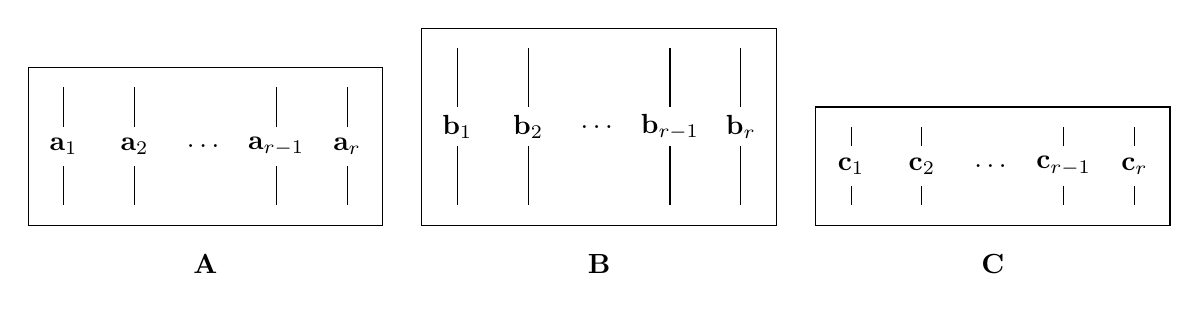
\begin{tikzpicture}[scale=1]
   \def\r{4.5}
   \def\ix{2.5}
   \def\iy{2}
   \def\iz{1.5}
   \def\distance{0.25}

   % Vertical bar height (how far above and below the label)
   \def\barheight{0.3}

  % Positions for each matrix
  \def\xA{0}
  \def\xB{\r+0.5}
  \def\xC{2*\r+1}

  % Draw rectangles for A, B, and C
  \draw (\xA,0) rectangle ++(\r,\iy);
  \draw (\xB,0) rectangle ++(\r,\ix);
  \draw (\xC,0) rectangle ++(\r,\iz);

  % Function to draw a vector column with bars above/below
  \newcommand{\vectorcolumn}[4]{
    \draw ({#1}, {#3 + \distance}) -- ({#1}, {#4 - \distance});
    \draw ({#1}, {#3 - \distance}) -- ({#1}, {0 + \distance});
    \node at (#1, #3) {#2};
  }

  % % First two columns: a_1, a_2
  % \foreach \i/\label in {0/1, 1/2} {
  %   \pgfmathsetmacro{\xai}{\xA + (\r/5)*(\i + 0.5)}
  %   \pgfmathsetmacro{\xbi}{\xB + (\r/5)*(\i + 0.5)}
  %   \pgfmathsetmacro{\xci}{\xC + (\r/5)*(\i + 0.5)}
  %   \vectorcolumn{\xai}{$\mathbf{a}_{\label}$}{0.5*\iy}
  %   \vectorcolumn{\xbi}{$\mathbf{b}_{\label}$}{0.5*\ix}
  %   \vectorcolumn{\xci}{$\mathbf{c}_{\label}$}{0.5*\iz}
  % }

  %  % Vector column macro with vertical lines
  %  \newcommand{\vectorcolumn}[5]{ % x, label, y_center, y_top, y_bottom
  %    % Top vertical line
  %    \draw ({#1}, {#3 + #5}) -- ({#1}, {#4 - #5});
  %    % Bottom vertical line
  %    \draw ({#1}, {#3 - #5}) -- ({#1}, {#2 + #5});
  %    % Label node
  %    \node at (#1, #3) {#2};
  %  }

   % First two columns
   \foreach \i/\label in {0/1, 1/2} {
     \pgfmathsetmacro{\xai}{\xA + (\r/5)*(\i + 0.5)}
     \pgfmathsetmacro{\yai}{0.5*\iy}
     \vectorcolumn{\xai}{$\mathbf{a}_{\label}$}{\yai}{\iy} % {\iy}{0.01}{\distance}

     \pgfmathsetmacro{\xbi}{\xB + (\r/5)*(\i + 0.5)}
     \pgfmathsetmacro{\ybi}{0.5*\ix}
     \vectorcolumn{\xbi}{$\mathbf{b}_{\label}$}{\ybi}{\ix} % {\ix}{0}{\distance}

     \pgfmathsetmacro{\xci}{\xC + (\r/5)*(\i + 0.5)}
     \pgfmathsetmacro{\yci}{0.5*\iz}
     \vectorcolumn{\xci}{$\mathbf{c}_{\label}$}{\yci}{\iz} % {\iz}{0}{\distance}
   }

   % Ellipsis column (centered)
   \node at ({\xA + (\r/5)*2.5}, {0.5*\iy}) {\ldots};
   \node at ({\xB + (\r/5)*2.5}, {0.5*\ix}) {\ldots};
   \node at ({\xC + (\r/5)*2.5}, {0.5*\iz}) {\ldots};

   % First two columns
   \foreach \i/\label in {3/{r-1}, 4/r} {
     \pgfmathsetmacro{\xai}{\xA + (\r/5)*(\i + 0.5)}
     \pgfmathsetmacro{\yai}{0.5*\iy}
     \vectorcolumn{\xai}{$\mathbf{a}_{\label}$}{\yai}{\iy} % {\iy}{0.01}{\distance}

     \pgfmathsetmacro{\xbi}{\xB + (\r/5)*(\i + 0.5)}
     \pgfmathsetmacro{\ybi}{0.5*\ix}
     \vectorcolumn{\xbi}{$\mathbf{b}_{\label}$}{\ybi}{\ix} % {\ix}{0}{\distance}

     \pgfmathsetmacro{\xci}{\xC + (\r/5)*(\i + 0.5)}
     \pgfmathsetmacro{\yci}{0.5*\iz}
     \vectorcolumn{\xci}{$\mathbf{c}_{\label}$}{\yci}{\iz} % {\iz}{0}{\distance}
   }

  % Matrix labels
  \node at ({\xA + 0.5*\r}, -0.5) {$\mathbf{A}$};
  \node at ({\xB + 0.5*\r}, -0.5) {$\mathbf{B}$};
  \node at ({\xC + 0.5*\r}, -0.5) {$\mathbf{C}$};

\end{tikzpicture}
            \caption[Kruskal Tensor Factor Matrices]{The vectors of the components of the Kruskal tensor come together to form factor matrices}
            \label{fig:KTensor_factor_matrices}
        \end{subfigure}
        \caption[The CP Decomposition]{The CP Decomposition}
    \end{figure}

    Mathematically, given a tensor $\mathcal{T} \in \mathbb{R}^{m\times n\times
    p}$ and decomposition rank $r\in \mathbb{N}$, the goal of a CP Decomposition
    is to find factor matrices $\mathbf{A}\in \mathbb{R}^{m\times r},
    \mathbf{B}\in \mathbb{R}^{n\times r}, \mathbf{C}\in \mathbb{R}^{p\times r}$
    such that \[ t_{ijk} \approx \sum_{\ell = 1}^{r} a_{i\ell}b_{j\ell}c_{k\ell}
    \text{, } \forall (i, j, k) \in [m]\times [n]\times [p] \] or alternatively
    \[ \mathcal{T} \approx \llbracket \mathbf{A, B, C} \rrbracket = \sum_{\ell =
    1}^{r} a_\ell \circ b_\ell \circ c_\ell.\]

    The memory footprint of a KTensor is $3rn$. The approximation gets more
    accurate as $r$ increases. This is the 2D matrix equivalent of having an
    $n\times n$ matrix approximation to be the sum of the outer product of two
    $n \times 1$ vectors. Traditional methods of computing the CP decomposition
    of a tensor are gradient descent and the Newton method. The method used in
    this work is a variation of the latter called damped Gauss-Newton (DGN).
    This method minimizes the sum of squares error seen in
    \Cref{eq:cp_least_squares}. 

    \begin{equation} \label{eq:cp_least_squares}
        \|\mathcal{T} - \llbracket \mathbf{A, B, C} \rrbracket \|^2 \equiv \sum_{i=1}^{m} \sum_{j=1}^{n} \sum_{k=1}^{p}\left(t_{ijk} - \sum_{\ell=1}^{r} a_{i\ell}b_{j\ell}c_{k\ell} \right)^2
    \end{equation}

    Thus, the CP optimization problem for a given $r$ is shown in
    \ref{eq:cp_opt}. This is a non-convex problem. 

    \begin{equation} \label{eq:cp_opt}
        \min \|\mathcal{T} - \llbracket \mathbf{A, B, C} \rrbracket \|^2 \text{, subject to } \mathbf{A} \in \mathbb{R}^{m\times r} \mathbf{B} \in \mathbb{R}^{n\times r} \mathbf{C} \in \mathbb{R}^{p\times r}
    \end{equation}
        




\subsection{Tucker Tensors and The Tucker Decomposition} \label{sec:Tucker Tensors and The Tucker Decomposition}
    The Tucker Decomposition compresses an input tensor into a Tucker Tensor
    (TTensor), which is a smaller core tensor with a factor matrix for each of
    its modes. To reconstruct the approximation of the original tensor, each
    factor matrix is multiplied with the core in its respective mode through a
    TTM. We can visualize this in the case of a 3-way tensor as shown in
    \Cref{fig:TTensor}.

    \begin{figure}[ht]
        \centering
        % 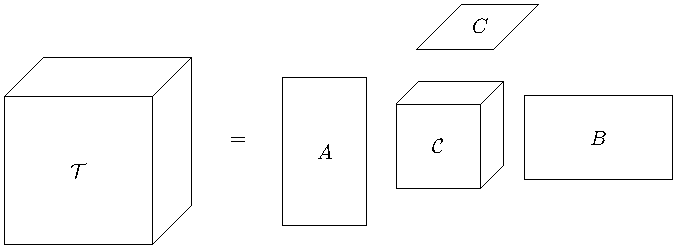
\includegraphics[scale=1]{tikz/chapter1/section1-2/Tucker_Tensor.pdf}
        % Mess with the first scale to change the size of your drawings
% Mess with the second scale to change the size of your letters
\begin{tikzpicture}[scale=1,namenode/.style={scale=1}]
   % These distances can be meddled with to get you what you want
   % Within reason...
   \def\ix{2.5} %
   \def\iy{2.5} %
   \def\iz{1.75} %
   \def\corescale{1.75} % Has to be more than 1
   \def\rot{90}
   \def\r{0.25}
   \def\rx{\ix/\corescale}
   \def\ry{\iy/\corescale}
   \def\rz{\iz/\corescale}
   
   % Give figure's starting point and draw a rectange
   \coordinate (TFrontLowerLeft) at (0,0);
   \draw (TFrontLowerLeft) rectangle ++ (\ix,\iy);

   % This scope draws the top face of the cube
   \begin{scope}[shift={(TFrontLowerLeft)}, canvas is zx plane at y=\iy,rotate=\rot]
      \draw (0,0) rectangle ++ (\ix,\iz);
   \end{scope}

   % This scope draws the left side of the cube
   \begin{scope}[shift={(TFrontLowerLeft)},canvas is zy plane at x=\ix,rotate=90]
      \draw (0,0) rectangle ++ (\iy,\iz); %
   \end{scope}

   % This writes the tensor name in the front face of the cube
   \node[namenode] at ($(TFrontLowerLeft) + (0.5*\ix, 0.5*\iy)$)  {$\mathbf{\mathcal{T}}$};

   % This writes the equal sign to the side of the cube
   \coordinate (ApproxCtr) at ($(TFrontLowerLeft) + (0.75+\ix+0.4*\iz,0.7*\iy)$);
   \node[namenode] at (ApproxCtr) {=};

   % First Factor Matrix
   \coordinate (AFrontLowerLeft) at ($(ApproxCtr) + (0.75,-\ry)$);
   \draw (AFrontLowerLeft) rectangle ++ (\rx,\iy);
   \node[namenode] at ($(AFrontLowerLeft) + (0.5*\rx, 0.5*\iy)$)  {$A$};

   % This scope draws the top face of the cube
   \coordinate (CFrontLowerLeft) at ($(AFrontLowerLeft) + (0.5 + \rx, 0.25*\ix)$);
   \draw (CFrontLowerLeft) rectangle ++ (\rx,\ry);
   
   \begin{scope}[shift={(CFrontLowerLeft)}, canvas is zx plane at y=\ry,rotate=\rot]
      \draw (0,0) rectangle ++ (\rx,\rz);
   \end{scope}

   % This scope draws the left side of the cube
   \begin{scope}[shift={(CFrontLowerLeft)},canvas is zy plane at x=\rx,rotate=90]
      \draw (0,0) rectangle ++ (\ry,\rz); %
   \end{scope}

   % This writes the core name in the front face of the cube
   \node[namenode] at ($(CFrontLowerLeft) + (0.5*\rx, 0.5*\ry)$)  {$\mathbf{\mathcal{G}}$};

   % Second Factor Matrix
   \coordinate (BFrontLowerLeft) at ($(CFrontLowerLeft) + (\rx + 0.75*\rz, 0.15*\rz)$);
   \draw (BFrontLowerLeft) rectangle ++ (\ix,\ry);
   \node[namenode] at ($(BFrontLowerLeft) + (0.5*\ix, 0.5*\ry)$)  {$B$};

   % Third Factor Matrix
   \begin{scope}[shift={($(CFrontLowerLeft) + (0.25*\rz,-0.25*\rz)$)},canvas is zx plane at y=\iy,rotate=90]
      \draw (0,\r) rectangle ++ (\rz*1.3,\iz*1.15);
   \end{scope}
   \node[namenode] at ($(CFrontLowerLeft) + (1*\rx,2.75*\rz)$) {$C$};

   
\end{tikzpicture}
        \caption[A 3-way Tucker Tensor Diagram]{A 3-way Tucker Tensor Diagram}
        \label{fig:TTensor}
    \end{figure}

    If we consider a 3D tensor of size $n^3$ with core of size $r^3$ where $r <
    n$, then the number of entries of a TTensor is $3rn + r^3$ which is less
    than the original memory footprint and much less if $r \ll n$. The
    reconstruction of the original tensor is performed using TTMs as seen in
    \ref{eq:tucker_ttm}, but if we wish to reconstruct but a single entry then
    we perform \ref{eq:tucker_element}

    \begin{equation} \label{eq:tucker_ttm}
        \mathcal{T} \approx \llbracket \mathcal{G}; \mathbf{A,B,C} \rrbracket = \mathcal{G} \times_1 \mathbf{A} \times_2 \mathbf{B} \times_3 \mathbf{C}
    \end{equation}
    
    \begin{equation} \label{eq:tucker_element}
        t_{ijk} = \sum_{\alpha = 1}^{q} \sum_{\beta = 1}^{r} \sum_{\gamma = 1}^{s} g_{\alpha \beta \gamma}\cdot a_{i\alpha}b_{j\beta}c_{i\gamma}\text{, }\forall (i, j, k) \in [m]\otimes[n]\otimes[p]
    \end{equation}
    
    
    The traditional methods are HOSVD (Higher Order Singular Value
    Decomposition) and STHOSVD (Sequentially Truncated Singular Value
    Decomposition). Though HOOI (Higher Order Orthogonal Iteration) is not as
    traditional, it will be the protagonist for this work. We describe these
    algorithms in \Cref{sec:Tucker Algorithms}

        \newpage





    %%%%%%%%%%%%%%%%%%%%%%%%%%%%%%%%%%%%%%
    %% Chapter 2 - The CP Decomposition %%
    %%%%%%%%%%%%%%%%%%%%%%%%%%%%%%%%%%%%%%
    \chapter{\textbf{The CP Decomposition}}
        %!TEX root = ../../main.tex

Despite the tile, the focus of this project are not CP Decompositions. Rather,
their active use in searching for fast matrix multiplication algorithms. There
was a glimpse of these types of algorithms in \Cref{sec:Matrix-Matrix Products},
but the rabbit hole goes deeper than that. Therefore, the use of CP
Decompositons of a special tensor to discover new fast matrix multiplication
algorithms is left for \Cref{sec:The Matrix Multiplication Tensor}, and
\Cref{sec:Fast Matrix Multiplication Algorithms} starts this chapter with some
much-needed background about Matrix Multiplication Algorithms.

% The goal for the first project is difficult to describe. Preliminary work on
% attempting to search for fast matrix multiplication algorithm shows that it is a
% daunting task. Even though exhaustive search is not enough to prove that an
% algorithm doesn't exist for certain ranks, it is clear that there are many more
% places where an algorithm fails to exist than the ones where it actually exists.
% But have implemented a new way of searching these algorithms much more
% efficiently than what was done in the past, and it could prove itself worthy of
% future use. We have more recently turned to a more mathematical approach to the
% project with the aid of Dr. Frank Moore and Dr. Pratyush Mishra. But where we
% are heading is still unknown. We wish to share some both the new method of
% searching for algorithm and some of the interesting solutions we found.

% The work done in the first project is more extensive. Recall that we can
% actively search for fast matrix multiplication algorithms by
% optimization as in \Cref{Opt}. We can do so by performing an CP
% Decomposition on the matrix multiplication tensor by specifying the size
% of the matrix $n$ and the number of multiplications in the algorithm
% $R$. This is described in algorithm \ref{alg:CP-DGN} where the details
% of how to compute the Function value, the gradient and the Jacobian are
% left as an exercise to the reader. But now, how do we modify it so that
% we can decrease the number of possibilities from $3^{84}$ to $3^{28}$ by
% relying on the cyclic invariance structure described earlier? The
% details of so can be seen in Algorithm \ref{alg:Mod-CP-DGN}. I once
% again leave the now much, much more complicated details of how to
% compute the function value, the gradient and the Jacobian as another
% exercise to the reader. 

\section{Matrix Multiplication Algorithms} \label{sec:Matrix Multiplication Algorithms}
    %!TEX root = ../../main.tex

\renewcommand{\arraystretch}{0.8} % adjust to make lines closer together

\subsection{Fast Matrix Multiplication Algorithms} \label{sec:Fast Matrix Multiplication Algorithms}

    Recall from \Cref{sec:Matrix-Matrix Products} the way matrix multiplications are
    performed. In fact, \Cref{eq:two_by_two_mat_mul} demonstrates how to multiply
    two matrices $\mathbf{A, B} \in \mathbb{R}^{2\times2}$. Matrices $\mathbf{A}$
    and $\mathbf{B}$ don't necessarily need to be of size 2 by 2, as long as they
    are of a size that is a multiple of 2, we can perform such matrix multiplication
    using a recursive algorithm like the one on \Cref{alg:recursive_mat_mul}. This
    is the only time such algorithm is presented using the pseudocode format, for
    the sake of simplicity algorithms will be showcased in the format displayed in
    \ref{eq:classic_matmul}.

    \begin{algorithm}[!ht]
        \caption{MatMul}
        \label{alg:recursive_mat_mul}
        \begin{algorithmic}[0]
            \Function{$\mathbf{C} = $ MatMul}{$\mathbf{A, B}$}
                \If{dim($\mathbf{A}$) = dim($\mathbf{A}$) = 1}
                    \State{\textbf{return} $\mathbf{A\cdot B}$}
                \EndIf
                \State{Divide into quadrants:
                    \(
                    \mathbf{A} =
                    \left[
                    \begin{array}{cc}
                        \mathbf{A}_{11} & \mathbf{A}_{12} \\
                        \mathbf{A}_{21} & \mathbf{A}_{22}
                    \end{array}
                    \right]
                    \mathbf{B} =
                    \left[
                    \begin{array}{cc}
                        \mathbf{B}_{11} & \mathbf{B}_{12} \\
                        \mathbf{B}_{21} & \mathbf{B}_{22}
                    \end{array}
                    \right]
                    \)
                }
                \State{$\mathbf{M}_1$ = MatMul($\mathbf{A_{11}, B_{11}}$)}
                \State{$\mathbf{M}_2$ = MatMul($\mathbf{A_{12}, B_{21}}$)}
                \State{$\mathbf{M}_3$ = MatMul($\mathbf{A_{11}, B_{12}}$)}
                \State{$\mathbf{M}_4$ = MatMul($\mathbf{A_{12}, B_{22}}$)}
                \State{$\mathbf{M}_5$ = MatMul($\mathbf{A_{21}, B_{21}}$)}
                \State{$\mathbf{M}_6$ = MatMul($\mathbf{A_{22}, B_{12}}$)}
                \State{$\mathbf{M}_7$ = MatMul($\mathbf{A_{21}, B_{12}}$)}
                \State{$\mathbf{M}_8$ = MatMul($\mathbf{A_{22}, B_{22}}$)}
                \vspace{10pt}
                \State{\textbf{return} \(
                    \mathbf{C} =
                    \left[
                    \begin{array}{cc}
                        \mathbf{M}_1 + \mathbf{M}_2 & \mathbf{M}_3 + \mathbf{M}_4 \\
                        \mathbf{M}_5 + \mathbf{M}_6 & \mathbf{M}_7 + \mathbf{M}_8 \\
                    \end{array}
                    \right]
                    \)
                }
            \EndFunction
        \end{algorithmic}
    \end{algorithm}


    \begin{center}
        \textbf{Classic 2 by 2 Matrix Multiplication Algorithm}
        \vspace{-20pt}
    \end{center}
    \begin{equation}
        \begin{array}{rcl}
            \color{blue} \mathbf{M}_1 & = & \mathbf{A}_{11}\cdot \mathbf{B}_{11} \\
            \color{blue} \mathbf{M}_2 & = & \mathbf{A}_{12}\cdot \mathbf{B}_{21} \\
            \color{blue} \mathbf{M}_3 & = & \mathbf{A}_{11}\cdot \mathbf{B}_{12} \\
            \color{blue} \mathbf{M}_4 & = & \mathbf{A}_{12}\cdot \mathbf{B}_{22} \\
            \color{blue} \mathbf{M}_5 & = & \mathbf{A}_{21}\cdot \mathbf{B}_{11} \\
            \color{blue} \mathbf{M}_6 & = & \mathbf{A}_{22}\cdot \mathbf{B}_{21} \\
            \color{blue} \mathbf{M}_7 & = & \mathbf{A}_{21}\cdot \mathbf{B}_{12} \\
            \color{blue} \mathbf{M}_8 & = & \mathbf{A}_{22}\cdot \mathbf{B}_{22} \\
            \mathbf{C}_{11} & = & \color{blue} \mathbf{M}_1 \color{black} + \color{blue} \mathbf{M}_2 \\
            \mathbf{C}_{12} & = & \color{blue} \mathbf{M}_3 \color{black} + \color{blue} \mathbf{M}_4 \\
            \mathbf{C}_{21} & = & \color{blue} \mathbf{M}_5 \color{black} + \color{blue} \mathbf{M}_6 \\
            \mathbf{C}_{22} & = & \color{blue} \mathbf{M}_7 \color{black} + \color{blue} \mathbf{M}_8
        \end{array}
        \label{eq:classic_matmul}
    \end{equation}


    This algorithm involves 8 multiplications and 4 additions of matrices of size
    $\nicefrac n2$. Therefore, our computational complexity becomes $T(n) =
    8T(\nicefrac{n}{2}) + O(n^2) = O(n^{\log_2 8}) = O(n^3)$. This computational
    cost can be decresed by carefully manipulating our multiplications and additions
    in order to reduce the number of recursive calls. In 1969, Volker Strassen
    became the first to develop an algorithm with cost less than $O(n^3)$, which
    made way for \textit{fast matrix multiplication algorithms}. His classic
    algorithm is showcased in \ref{eq:classic_strassen}. His algorithm involves 7
    multiplications and 18 additions, but recall that additions are computationally
    less expensive than multiplications. The computational complexity of Strassen's
    algorithm is $T(n) = 7T(\nicefrac n2) + O(n^2) = O(n^{\log_2 7}) \approx O(n^{2.81})$. 

    \begin{center}
        \textbf{Classic Strassen's Algorithm}
        \vspace{-20pt}
    \end{center}
    \begin{equation}
        \begin{array}{rcl}
            \color{blue} \mathbf{M}_1 & = & (\mathbf{A}_{11} + \mathbf{A}_{22})\cdot (\mathbf{B}_{11} + \mathbf{B}_{22}) \\
            \color{blue} \mathbf{M}_2 & = & (\mathbf{A}_{12} + \mathbf{A}_{22})\cdot \mathbf{B}_{11} \\
            \color{blue} \mathbf{M}_3 & = & \mathbf{A}_{11}\cdot (\mathbf{B}_{21} - \mathbf{B}_{22}) \\
            \color{blue} \mathbf{M}_4 & = & \mathbf{A}_{22}\cdot (\mathbf{B}_{12} - \mathbf{B}_{11}) \\
            \color{blue} \mathbf{M}_5 & = & (\mathbf{A}_{11} + \mathbf{A}_{21})\cdot B_{22} \\
            \color{blue} \mathbf{M}_6 & = & (\mathbf{A}_{12} - \mathbf{A}_{11})\cdot (\mathbf{B}_{11} + \mathbf{B}_{21}) \\
            \color{blue} \mathbf{M}_7 & = & (\mathbf{A}_{21} - \mathbf{A}_{22})\cdot (\mathbf{B}_{12} + \mathbf{B}_{22}) \\
            \mathbf{C}_{11} & = & \color{blue} \mathbf{M}_1 \color{black} + \color{blue} \mathbf{M}_4 \color{black} - \color{blue} \mathbf{M}_5 \color{black} + \color{blue} \mathbf{M}_7 \\
            \mathbf{C}_{12} & = & \color{blue} \mathbf{M}_3 \color{black} + \color{blue} \mathbf{M}_5 \\
            \mathbf{C}_{21} & = & \color{blue} \mathbf{M}_2 \color{black} + \color{blue} \mathbf{M}_4 \\
            \mathbf{C}_{22} & = & \color{blue} \mathbf{M}_1 \color{black} - \color{blue} \mathbf{M}_2 \color{black} + \color{blue} \mathbf{M}_3 \color{black} + \color{blue} \mathbf{M}_6
        \end{array}
        \label{eq:classic_strassen}
    \end{equation}



    Strassen's algorithm is not unique. We can rearrange and slighlty modify the
    additions and multiplies to get another algorithm with the same number of
    multiplies and additions. An example of these variations of Strassen's
    algorithms can be seen in \ref{eq:var_strassen}. 

    \begin{center}
        \textbf{Variant Strassen's Algorithm}
        \vspace{-20pt}
    \end{center}
    \begin{equation}
        \begin{array}{rcl}
            \color{blue} \mathbf{M}_1 & = & (\mathbf{A}_{11} + \mathbf{A}_{22})\cdot (\mathbf{B}_{11} + \mathbf{B}_{22}) \\
            \color{blue} \mathbf{M}_2 & = & (\mathbf{A}_{12} + \mathbf{A}_{22})\cdot \mathbf{B}_{11} \\
            \color{blue} \mathbf{M}_3 & = & \mathbf{A}_{22}\cdot (\mathbf{B}_{12} - \mathbf{B}_{11}) \\
            \color{blue} \mathbf{M}_4 & = & (\mathbf{A}_{21} - \mathbf{A}_{22})\cdot (\mathbf{B}_{12} + \mathbf{B}_{22}) \\
            \color{blue} \mathbf{M}_5 & = & (\mathbf{A}_{11} + \mathbf{A}_{21})\cdot \mathbf{B}_{22} \\
            \color{blue} \mathbf{M}_6 & = & \mathbf{A}_{11}\cdot (\mathbf{B}_{21} - \mathbf{B}_{22}) \\
            \color{blue} \mathbf{M}_7 & = & (\mathbf{A}_{12} - \mathbf{A}_{11})\cdot (\mathbf{B}_{11} + \mathbf{B}_{21}) \\
            \mathbf{C}_{11} & = & \color{blue} \mathbf{M}_1 \color{black} + \color{blue} \mathbf{M}_3 \color{black} - \color{blue} \mathbf{M}_4 \color{black} - \color{blue} \mathbf{M}_6 \\
            \mathbf{C}_{12} & = & \color{blue} \mathbf{M}_2 \color{black} + \color{blue} \mathbf{M}_3 \\
            \mathbf{C}_{21} & = & \color{blue} \mathbf{M}_5 \color{black} + \color{blue} \mathbf{M}_6 \\
            \mathbf{C}_{22} & = & \color{blue} \mathbf{M}_1 \color{black} - \color{blue} \mathbf{M}_2 \color{black} + \color{blue} \mathbf{M}_5 \color{black} + \color{blue} \mathbf{M}_7
        \end{array}
        \label{eq:var_strassen}
    \end{equation}

    It is at this point that an important distinction must be made; what is
    considered a new algorithm? Both Strassen's algorithm and the variant presented
    are considered Strassen's algorithm because they both involve 7 multiplications.
    This is because the term \textit{Strassen's algorithm} has become an
    all-encapsulating term for any 2 by 2 matrix multiplication algorithm that uses
    7 multiplications instead of the classic 8. If we wish to be precise, the
    algorithm presented in \ref{eq:classic_strassen} is the one and only original
    algorithm and all other variations are different algorithms that also happen to
    have 7 multiplications and, like previously mentioned, historically any
    algorithm with 7 multiplications are referred to Strassen's algorithm. It can
    get confusing, but any functioning variant of Strassen's algorithm is Strassen's
    algorithm despite them having distinct order of multiplications and additions.
    Thus, a question arises, how many possibilities are there? We could search for
    different solutions that all have the same number of multiplications by
    performing either an eshaustive search or an optimization search on each
    parameter involved in matrix multiplication as seen in
    \ref{eq:serching_fast_matmul}. If we are searching for a discrete solution with
    only -1, 0, 1 as coefficients then we have $3^84$ possibilities, though not all
    of these possibilities would be valid algotithms.


    \begin{center}
        \textbf{Exhaustive Search of Fast MatMul Algorithms}
        \vspace{-20pt}
    \end{center}
    \begin{equation}
        \scalebox{0.9}{
            $\displaystyle
            \begin{array}{rcl}
                \color{blue} \mathbf{M}_1 & = & (\textcolor{purple}{ u_{11}^{(1)}} \mathbf{A}_{11} + \textcolor{purple}{u_{12}^{(1)}} \mathbf{A}_{12} + \textcolor{purple}{ u_{21}^{(1)}} \mathbf{A}_{21} + \textcolor{purple}{ u_{22}^{(1)}} \mathbf{A}_{22}) \cdot (\textcolor{purple}{ v_{11}^{(1)}} \mathbf{B}_{11} + \textcolor{purple}{v_{12}^{(1)}} \mathbf{B}_{12} + \textcolor{purple}{v_{21}^{(1)}} \mathbf{B}_{21} \textcolor{purple}{ v_{22}^{(1)}} \mathbf{B}_{22}) \\
                \color{blue} \mathbf{M}_2 & = & (\textcolor{purple}{ u_{11}^{(2)}} \mathbf{A}_{11} + \textcolor{purple}{u_{12}^{(2)}} \mathbf{A}_{12} + \textcolor{purple}{ u_{21}^{(2)}} \mathbf{A}_{21} + \textcolor{purple}{ u_{22}^{(2)}} \mathbf{A}_{22}) \cdot (\textcolor{purple}{ v_{11}^{(2)}} \mathbf{B}_{11} + \textcolor{purple}{v_{12}^{(2)}} \mathbf{B}_{12} + \textcolor{purple}{v_{21}^{(2)}} \mathbf{B}_{21} \textcolor{purple}{ v_{22}^{(2)}} \mathbf{B}_{22}) \\
                \color{blue} \mathbf{M}_3 & = & (\textcolor{purple}{ u_{11}^{(3)}} \mathbf{A}_{11} + \textcolor{purple}{u_{12}^{(3)}} \mathbf{A}_{12} + \textcolor{purple}{ u_{21}^{(3)}} \mathbf{A}_{21} + \textcolor{purple}{ u_{22}^{(3)}} \mathbf{A}_{22}) \cdot (\textcolor{purple}{ v_{11}^{(3)}} \mathbf{B}_{11} + \textcolor{purple}{v_{12}^{(3)}} \mathbf{B}_{12} + \textcolor{purple}{v_{21}^{(3)}} \mathbf{B}_{21} \textcolor{purple}{ v_{22}^{(3)}} \mathbf{B}_{22}) \\
                \color{blue} \mathbf{M}_4 & = & (\textcolor{purple}{ u_{11}^{(4)}} \mathbf{A}_{11} + \textcolor{purple}{u_{12}^{(4)}} \mathbf{A}_{12} + \textcolor{purple}{ u_{21}^{(4)}} \mathbf{A}_{21} + \textcolor{purple}{ u_{22}^{(4)}} \mathbf{A}_{22}) \cdot (\textcolor{purple}{ v_{11}^{(4)}} \mathbf{B}_{11} + \textcolor{purple}{v_{12}^{(4)}} \mathbf{B}_{12} + \textcolor{purple}{v_{21}^{(4)}} \mathbf{B}_{21} \textcolor{purple}{ v_{22}^{(4)}} \mathbf{B}_{22}) \\
                \color{blue} \mathbf{M}_5 & = & (\textcolor{purple}{ u_{11}^{(5)}} \mathbf{A}_{11} + \textcolor{purple}{u_{12}^{(5)}} \mathbf{A}_{12} + \textcolor{purple}{ u_{21}^{(5)}} \mathbf{A}_{21} + \textcolor{purple}{ u_{22}^{(5)}} \mathbf{A}_{22}) \cdot (\textcolor{purple}{ v_{11}^{(5)}} \mathbf{B}_{11} + \textcolor{purple}{v_{12}^{(5)}} \mathbf{B}_{12} + \textcolor{purple}{v_{21}^{(5)}} \mathbf{B}_{21} \textcolor{purple}{ v_{22}^{(5)}} \mathbf{B}_{22}) \\
                \color{blue} \mathbf{M}_6 & = & (\textcolor{purple}{ u_{11}^{(6)}} \mathbf{A}_{11} + \textcolor{purple}{u_{12}^{(6)}} \mathbf{A}_{12} + \textcolor{purple}{ u_{21}^{(6)}} \mathbf{A}_{21} + \textcolor{purple}{ u_{22}^{(6)}} \mathbf{A}_{22}) \cdot (\textcolor{purple}{ v_{11}^{(6)}} \mathbf{B}_{11} + \textcolor{purple}{v_{12}^{(6)}} \mathbf{B}_{12} + \textcolor{purple}{v_{21}^{(6)}} \mathbf{B}_{21} \textcolor{purple}{ v_{22}^{(6)}} \mathbf{B}_{22}) \\
                \color{blue} \mathbf{M}_7 & = & (\textcolor{purple}{ u_{11}^{(7)}} \mathbf{A}_{11} + \textcolor{purple}{u_{12}^{(7)}} \mathbf{A}_{12} + \textcolor{purple}{ u_{21}^{(7)}} \mathbf{A}_{21} + \textcolor{purple}{ u_{22}^{(7)}} \mathbf{A}_{22}) \cdot (\textcolor{purple}{ v_{11}^{(7)}} \mathbf{B}_{11} + \textcolor{purple}{v_{12}^{(7)}} \mathbf{B}_{12} + \textcolor{purple}{v_{21}^{(7)}} \mathbf{B}_{21} \textcolor{purple}{ v_{22}^{(7)}} \mathbf{B}_{22}) \\ \\
                \mathbf{C}_{11} & = & \textcolor{purple}{w_{11}^{(1)}} \color{blue} \mathbf{M}_1 + \textcolor{purple}{w_{11}^{(2)}} \color{blue} \mathbf{M}_2 + \textcolor{purple}{w_{11}^{(3)}} \color{blue} \mathbf{M}_3 + \textcolor{purple}{w_{11}^{(4)}} \color{blue} \mathbf{M}_4 + \textcolor{purple}{w_{11}^{(5)}} \color{blue} \mathbf{M}_5 + \textcolor{purple}{w_{11}^{(6)}} \color{blue} \mathbf{M}_6 + \textcolor{purple}{w_{11}^{(7)}} \color{blue} \mathbf{M}_7 \\
                \mathbf{C}_{12} & = & \textcolor{purple}{w_{12}^{(1)}} \color{blue} \mathbf{M}_1 + \textcolor{purple}{w_{12}^{(2)}} \color{blue} \mathbf{M}_2 + \textcolor{purple}{w_{12}^{(3)}} \color{blue} \mathbf{M}_3 + \textcolor{purple}{w_{12}^{(4)}} \color{blue} \mathbf{M}_4 + \textcolor{purple}{w_{12}^{(5)}} \color{blue} \mathbf{M}_5 + \textcolor{purple}{w_{12}^{(6)}} \color{blue} \mathbf{M}_6 + \textcolor{purple}{w_{12}^{(7)}} \color{blue} \mathbf{M}_7 \\
                \mathbf{C}_{21} & = & \textcolor{purple}{w_{21}^{(1)}} \color{blue} \mathbf{M}_1 + \textcolor{purple}{w_{21}^{(2)}} \color{blue} \mathbf{M}_2 + \textcolor{purple}{w_{21}^{(3)}} \color{blue} \mathbf{M}_3 + \textcolor{purple}{w_{21}^{(4)}} \color{blue} \mathbf{M}_4 + \textcolor{purple}{w_{21}^{(5)}} \color{blue} \mathbf{M}_5 + \textcolor{purple}{w_{21}^{(6)}} \color{blue} \mathbf{M}_6 + \textcolor{purple}{w_{21}^{(7)}} \color{blue} \mathbf{M}_7 \\
                \mathbf{C}_{22} & = & \textcolor{purple}{w_{22}^{(1)}} \color{blue} \mathbf{M}_1 + \textcolor{purple}{w_{22}^{(2)}} \color{blue} \mathbf{M}_2 + \textcolor{purple}{w_{22}^{(3)}} \color{blue} \mathbf{M}_3 + \textcolor{purple}{w_{22}^{(4)}} \color{blue} \mathbf{M}_4 + \textcolor{purple}{w_{22}^{(5)}} \color{blue} \mathbf{M}_5 + \textcolor{purple}{w_{22}^{(6)}} \color{blue} \mathbf{M}_6 + \textcolor{purple}{w_{22}^{(7)}} \color{blue} \mathbf{M}_7 \\
            \end{array}
            $
        }
        \label{eq:serching_fast_matmul}
    \end{equation}

\subsection{The Matrix Multiplication Tensor} \label{sec:The Matrix Multiplication Tensor}

    There is a specific type of tensor that is crucial to this project: the
    Matrix Multiplication Tensor. Matrix multiplication can be performed in
    tensor format using this tensor. If we wish to multiply two matrices
    $\mathbf{A} \in \mathbb{R}^{m\times n}$ and $\mathbf{B}\in
    \mathbb{R}^{n\times p}$, we can form the respective matrix multiplication
    tensor $\mathcal{M}\in \mathbb{R}^{mn \times np\times mp}$ through
    \Cref{alg:matmul_tensor}. In order to do so, we vectorize $\mathbf{A}$ and
    $\mathbf{B}$ and multiply them through TTMs in the first and second mode
    respectively. The output, in the third mode, is the vectorization of the
    output $\mathbf{C} = \mathbf{A}\cdot \mathbf{B}$ transposed (i.e.
    $\mathbf{C^\intercal}$). This project is concerned only with square
    matrices, thus we always assume $\mathbf{A}, \mathbf{B}, \mathbf{C}\in
    \mathbb{R}^{n\times n}$ and $\mathcal{M}\in\mathbb{R}^{n^2\times n^2\times
    n^2}$. We can visualize such product in \Cref{fig:matmul_tensor}. 

    \begin{algorithm}
        \caption{Create MatMul Tensor}
        \label{alg:matmul_tensor}
        \begin{algorithmic}[0]
            \Function{$\mathcal{T}$ = MatMul-Tensor}{$m, n, p$}
                \State{$\mathcal{T}$ = \texttt{zeros}($mn, np, mp$)} \Comment{Initialize Tensor}
                \For{$i = 1:m$}
                    \For{$i = 1:m$}
                        \For{$i = 1:m$}
                            \State{$\mathcal{T}(mj + i, nk + j, pi + k) = 1$}
                        \EndFor
                    \EndFor
                \EndFor
            \EndFunction
        \end{algorithmic}
    \end{algorithm}

    \begin{figure}
        \centering
        \begin{tikzpicture}[scale=1,namenode/.style={scale=1}]
    % These distances can be meddled with to get you what you want
    % Within reason...
    \def\ix{2} %
    \def\iy{2} %
    \def\iz{2} %
    \def\r{\iz/4}
    \def\corescale{1.75}
    \def\rx{\ix/\corescale}
    \def\ry{\iy/\corescale}
    \def\rz{\iz/\corescale}
    \def\sp{\rx/6}
    
    % This line chooses the starting location of the object
    \coordinate (MFrontLowerLeft) at (0,0);

    % This draws the front og the cube
    \draw (MFrontLowerLeft) rectangle ++ (\ix,\iy);

    % This scope draws the top face of the cube
    \begin{scope}[shift={(MFrontLowerLeft)}, canvas is zx plane at y=\iy,rotate=90]
        \draw (0,0) rectangle ++ (\ix,\iz);
    \end{scope}

    % This scope draws the left side of the cube
    \begin{scope}[shift={(MFrontLowerLeft)},canvas is zy plane at x=\ix,rotate=90]
        \draw (0,0) rectangle ++ (\iy,\iz); %
    \end{scope}

    % This writes the M in the front face of the cube
    \node[namenode] at ($(MFrontLowerLeft) + (0.5*\ix, 0.5*\iy)$)  {$\mathcal{M}$};

    \coordinate (ALowerLeft) at ($(MFrontLowerLeft) + (-\ix - 0.5, \iy-\r/1.5)$);
    \draw (ALowerLeft) rectangle ++ (\iy, \r/1.25);
    \node[namenode] at ($(ALowerLeft) + (\iy/2, 0.2)$) {$A$};

    \coordinate (BLowerLeft) at ($(MFrontLowerLeft) + (\ix+1.15,0.775)$);
    \draw (BLowerLeft) rectangle ++ (\r/1.25, \iy);
    \node[namenode] at ($(BLowerLeft) + (0.19, \iy/2)$) {$B$};

    \coordinate (L1) at ($(MFrontLowerLeft) + (\ix + \sp, \sp)$);
    \coordinate (L1H) at ($(L1) + (0, \iy)$);
    \draw[thin, densely dotted] (L1) -- (L1H);
    \coordinate (L1) at ($(MFrontLowerLeft) + (\ix + 2*\sp, 2*\sp)$);
    \coordinate (L1H) at ($(L1) + (0, \iy)$);
    \draw[thin, densely dotted] (L1) -- (L1H);
    \coordinate (L1) at ($(MFrontLowerLeft) + (\ix + 3*\sp, 3*\sp)$);
    \coordinate (L1H) at ($(L1) + (0, \iy)$);
    \draw[thin, densely dotted] (L1) -- (L1H);
    
    \coordinate (L1) at ($(MFrontLowerLeft) + (\sp, \iy + \sp)$);
    \coordinate (L1H) at ($(L1) + (\ix, 0)$);
    \draw[thin, densely dotted] (L1) -- (L1H);
    \coordinate (L1) at ($(MFrontLowerLeft) + (2*\sp, \iy + 2*\sp)$);
    \coordinate (L1H) at ($(L1) + (\ix, 0)$);
    \draw[thin, densely dotted] (L1) -- (L1H);
    \coordinate (L1) at ($(MFrontLowerLeft) + (3*\sp, \iy + 3*\sp)$);
    \coordinate (L1H) at ($(L1) + (\ix, 0)$);
    \draw[thin, densely dotted] (L1) -- (L1H);

    \node[namenode] at ($(MFrontLowerLeft) + (3.25+0.5*\ix, 0.5*\iy)$)  {$ = $};

    % This scope draws the top face of the cube
    \coordinate (CLowerLeft) at ($(MFrontLowerLeft) + (4.85, -\iy/3)$);
    \begin{scope}[shift={(CLowerLeft)}, canvas is zx plane at y=\iy,rotate=90]
        \draw (0,0) rectangle ++ (\r/1.25, \ix);
    \end{scope}

    \node[namenode] at ($(CLowerLeft) + (1.25, \iy + 0.3)$) {$C^\text{T}$};
\end{tikzpicture}
        \caption{Matrix Multiplication in Tensor Format}
        \label{fig:matmul_tensor}
    \end{figure}

    It is at this point we return to tensor decompositions, specifically the CP
    decomposition. Recall from \ref{sec:Kruskal Tensors and The CP
    Decomposition} that the decomposition compresses an input tensor into $r$
    $d$-way outer product components. It turns out, that if we decompose the
    matrix multiplication tensor using the CP Decomposition, there is a hidden
    fast matrix multiplication algorithm embedded in the components of the CP
    decomposition. In fact, the number of components $r$ corresponds to the
    number of multiplications in the algorithm. This in return results in two
    different implications, really you could argue that they mean the same thing
    in two different directions, but we seperate these implications for the sake
    of understanding. The first implication is that given an algorithm, say one
    of the $3^84$ for $2\times 2$ algorithms with rank 7, we can form the
    KTensor of the corresponding algorithm, namely $\mathcal{\hat{M}}$ and take
    the norm of the difference from the original matmul tensor. If $\|\mathcal{M
    - \hat{M}} = 0$, then we have a valid algorithm. Below is the original
    Strassen's algorithm with two representations, the one we have seen before
    and the KTensor representation. The way to interpret the algorithm on the
    right, is that each horizontal lines separate the factor matrices, therefore
    just like in \Cref{fig:KTensor} the factor matrices $\mathbf{A}, \mathbf{B}$
    and $\mathbf{C}$ are separated by the horizontal lines, the columns of the
    factor matrices represent the chicken feet components. If you pay close
    attention you can see how the columns representing $\mathbf{M}_\ell$
    correspond to the representation on the right. If a 1 or -1 appear in the
    right representation then they appear as $\mathbf{A}_{ij}$ or
    $\mathbf{-A}_{ij}$ respectively on the left. 

    \vspace{-50pt}
    \begin{multicols}{2}
        \begin{equation*}
            \begin{array}{rcl}
                \color{blue} \mathbf{M}_1 & = & (\mathbf{A}_{11} + \mathbf{A}_{22})\cdot (\mathbf{B}_{11} + \mathbf{B}_{22}) \\
                \color{blue} \mathbf{M}_2 & = & (\mathbf{A}_{12} + \mathbf{A}_{22})\cdot \mathbf{B}_{11} \\
                \color{blue} \mathbf{M}_3 & = & \mathbf{A}_{11}\cdot (\mathbf{B}_{21} - \mathbf{B}_{22}) \\
                \color{blue} \mathbf{M}_4 & = & \mathbf{A}_{22}\cdot (\mathbf{B}_{12} - \mathbf{B}_{11}) \\
                \color{blue} \mathbf{M}_5 & = & (\mathbf{A}_{11} + \mathbf{A}_{21})\cdot B_{22} \\
                \color{blue} \mathbf{M}_6 & = & (\mathbf{A}_{12} - \mathbf{A}_{11})\cdot (\mathbf{B}_{11} + \mathbf{B}_{21}) \\
                \color{blue} \mathbf{M}_7 & = & (\mathbf{A}_{21} - \mathbf{A}_{22})\cdot (\mathbf{B}_{12} + \mathbf{B}_{22}) \\
                \mathbf{C}_{11} & = & \color{blue} \mathbf{M}_1 \color{black} + \color{blue} \mathbf{M}_4 \color{black} - \color{blue} \mathbf{M}_5 \color{black} + \color{blue} \mathbf{M}_7 \\
                \mathbf{C}_{12} & = & \color{blue} \mathbf{M}_3 \color{black} + \color{blue} \mathbf{M}_5 \\
                \mathbf{C}_{21} & = & \color{blue} \mathbf{M}_2 \color{black} + \color{blue} \mathbf{M}_4 \\
                \mathbf{C}_{22} & = & \color{blue} \mathbf{M}_1 \color{black} - \color{blue} \mathbf{M}_2 \color{black} + \color{blue} \mathbf{M}_3 \color{black} + \color{blue} \mathbf{M}_6
            \end{array}
        \end{equation*}

        \columnbreak

        \setlength{\arraycolsep}{3pt}
        \[\begin{array}{c|ccccccc}
            & \color{blue} \mathbf{M}_1 & \color{blue} \mathbf{M}_2 & \color{blue} \mathbf{M}_3 & \color{blue} \mathbf{M}_4 & \color{blue} \mathbf{M}_5 & \color{blue} \mathbf{M}_6 & \color{blue} \mathbf{M}_7 \\
            \hline
            \mathbf{A}_{11} & 1 & 0 & 1 & 0 & 1 & -1 & 0 \\
            \mathbf{A}_{12} & 0 & 1 & 0 & 0 & 0 & 1 & 0 \\
            \mathbf{A}_{21} & 0 & 0 & 0 & 0 & 1 & 0 & 1 \\
            \mathbf{A}_{22} & 1 & 1 & 0 & 1 & 0 & 0 & -1 \\
            \hline
            \mathbf{B}_{11} & 1 & 1 & 0 & -1 & 0 & 1 & 0 \\
            \mathbf{B}_{12} & 0 & 0 & 0 & 1 & 0 & 0 & 1 \\
            \mathbf{B}_{21} & 0 & 0 & 1 & 0 & 0 & 1 & 0 \\
            \mathbf{B}_{22} & 1 & 0 & -1 & 0 & 1 & 0 & 1 \\
            \hline
            \mathbf{C}_{11} & 1 & 0 & 0 & 1 & -1 & 0 & 1 \\
            \mathbf{C}_{21} & 0 & 0 & 1 & 0 & 1 & 0 & 0 \\
            \mathbf{C}_{12} & 0 & 1 & 0 & 1 & 0 & 0 & 0 \\
            \mathbf{C}_{22} & 1 & -1 & 1 & 0 & 0 & 1 & 0 \\
    \end{array}\]
    \end{multicols}
    
    
    The other implication, is that we can decompose the matmul tensor with
    specified CP rank through (as in \Cref{eq:cp_opt}) an optimization
    algorithmto search for fast matrix multiplication algorithms. Now how do we
    do that?






\subsection{Damped Gauss Newton Optimization for CP Decompositions}\label{sec:Damped Gauss Newton Optimization for CP Decompositions}
    
    Recall from \Cref{eq:cp_least_squares} that we perform a CP decomposition
    with the least squares error of our approximation. We will do so using
    optimization methods for reasons that will become clear soon. Optimization
    methods work with vector input, so for our purposes let 

    \begin{equation*}
        \mathbf{v} = \text{vec}
        \left(
        \left[
            \begin{array}{c}
                \mathbf{A} \\
                \mathbf{B} \\
                \mathbf{C}
            \end{array}
        \right]
        \right) = 
        \left[
            \begin{array}{c}
                \text{vec}(\mathbf{A}) \\
                \text{vec}(\mathbf{B}) \\
                \text{vec}(\mathbf{C})
            \end{array}
        \right]
        \in \mathbb{R}^{3nr}
    \end{equation*}

    Furthermore, let $\phi: \mathbb{R}^n \to \mathbb{R}^m$ be the nonlinear
    function. 

    \begin{equation}
        \phi (\mathbf{v}) = \text{vec}(\mathcal{M} - \llbracket \mathbf{A, B, C} \rrbracket)
    \end{equation}

    Thus, \Cref{eq:cp_least_squares} becomes 

    \begin{equation}
        \min_{A, B, C} f(\mathbf{v}) = \frac{1}{2} \|\phi (\mathbf{v})\|^2
    \end{equation}

    With that out of the way we must choose an optimization method. Gradient is
    too simple, taking one step further we reach Newton's method. Newton's
    mathod gets the search direction by using Newton's equation
    \[\nabla^2 f(\mathbf{v})\mathbf{d}_k = -\nabla f(\mathbf{v})\] We dislike
    the Hessian here because it is computationally expensive and difficult to
    derive mathematicall (perhaps not now but for the cylic part). Thus, we
    prefer the Gauss-Newton method which approximates the Hessian with
    $\mathbf{J^\intercal J}$ where $\mathbf{J}: \mathbb{R}^n\to
    \mathbb{R}^{n\times m}$ is the jacobian of $\phi$: \[(\mathbf{J^\intercal
    J})\mathbf{d}_k = -\nabla f(\mathbf{v})\] But even then, the Gauss-Newton
    matrix $\mathbf{J^\intercal J}$ can be singular, we add a damping parameter,
    $\lambda \mathbf{I}$, to enforce positive definiteness. Thus, we reach the
    damped Gauss-Newton Method: \[(\mathbf{J^\intercal J} +
    \lambda\mathbf{I})\mathbf{d}_k = -\nabla f(\mathbf{v})\]. At this point, we
    have two tasks at hand, given our $\mathbf{v}, f(\mathbf{v})$ and
    $\phi(\mathbf{v})$. We must derive the gradient of $f$ for the right-hand
    side and the jacobian of $\phi$ for the left-hand side (when really we just
    want to know how to apply it to a vector). The gradient is easy. 

    \begin{equation} \label{eq:cp_dgn_gradient}
        \nabla f = \text{vec}
        \left(
        \left[
        \begin{array}{c}
            \frac{\partial f}{\partial \mathbf{A}} \\
            \frac{\partial f}{\partial \mathbf{B}} \\
            \frac{\partial f}{\partial \mathbf{C}}
        \end{array}
        \right]
        \right) = 
        \left[
            \begin{array}{c}
                \frac{\partial f}{\partial \text{vec}(\mathbf{A})} \\
                \frac{\partial f}{\partial \text{vec}(\mathbf{B})} \\
                \frac{\partial f}{\partial \text{vec}(\mathbf{C})}
            \end{array}
        \right]
        \in \mathbb{R}^{3nr}
    \end{equation}

    Where each partial derivative is defined as:

    \begin{equation}
        \begin{array}{rcl}
            \frac{\partial f}{\partial \mathbf{A}} & = & -\mathbf{M}_{(1)}(\mathbf{C\odot B}) + \mathbf{A(C^\intercal C\ast B^\intercal B)} \\ 
            \frac{\partial f}{\partial \mathbf{B}} & = & -\mathbf{M}_{(1)}(\mathbf{C\odot A}) + \mathbf{B(C^\intercal C\ast A^\intercal A)} \\ 
            \frac{\partial f}{\partial \mathbf{C}} & = & -\mathbf{M}_{(1)}(\mathbf{B\odot A}) + \mathbf{C(B^\intercal B\ast A^\intercal A)} 
        \end{array}
        \label{eq:cp_dgn_partials}
    \end{equation}
    
    The Jacobian is not so easy. 
    
    \begin{equation} \label{eq:cp_dgn_jacobian}
        \mathbf{J} = [\mathbf{J}_\mathbf{A} + \mathbf{J}_\mathbf{B} + \mathbf{J}_\mathbf{C}] \in \mathbb{R}^{n^3\times 3nr}
    \end{equation}
    
    Where
    
    \begin{equation}
        \begin{array}{rcl}
            \mathbf{J}_\mathbf{A} \equiv \frac{\partial \phi}{\partial \text{vec}(\mathbf{A})} = (\mathbf{C} \odot \mathbf{B}) \otimes \mathbf{I} \in \mathbb{R}^{n^3\times nr} \\
            \mathbf{J}_\mathbf{B} \equiv \frac{\partial \phi}{\partial \text{vec}(\mathbf{B})} = \mathbf{\Pi}_2^\intercal (\mathbf{C} \odot \mathbf{A}) \otimes \mathbf{I} \in \mathbb{R}^{n^3\times nr} \\
            \mathbf{J}_\mathbf{C} \equiv \frac{\partial \phi}{\partial \text{vec}(\mathbf{C})} = \mathbf{\Pi}_3^\intercal(\mathbf{B} \odot \mathbf{A}) \otimes \mathbf{I} \in \mathbb{R}^{n^3\times nr}
        \end{array}
        \label{eq:cp_dgn_jacobians}
    \end{equation}

    such that that $\Pi_k$ is the tensor perfect shuffle matrix, such that
    vec($\mathcal{X}$) = $\Pi_k$ vec($\mathbf{X}_{(k)}$), and $\Pi_1$ is not
    written explicitly because it is the identity matrix. We consider fast
    computation of $\mathbf{J^\intercal J} + \lambda \mathbf{I}$. Rather than
    forming $\mathbf{J}$ or $\mathbf{J^\intercal J}$ explicitly, we use the
    structure of these matrices to compute the matrix-vector product without
    computing any explicit Kronecker or Khatri-Rao products. From
    \Cref{eq:cp_dgn_jacobian} we have that the block structure of
    $\mathbf{J^\intercal J}$ is 

    \begin{equation*}
        \mathbf{J^\intercal J} = 
        \left[
        \begin{array}{ccc}
            \mathbf{J_A^\intercal J_A} & \mathbf{J_A^\intercal J_B} & \mathbf{J_A^\intercal J_C} \\ 
            \mathbf{J_B^\intercal J_A} & \mathbf{J_B^\intercal J_B} & \mathbf{J_B^\intercal J_C} \\ 
            \mathbf{J_C^\intercal J_A} & \mathbf{J_C^\intercal J_B} & \mathbf{J_C^\intercal J_C} 
        \end{array}
        \right]
    \end{equation*}
    
    then
    
    \begin{equation*}
        \mathbf{J^\intercal Jv} = 
        \left[
        \begin{array}{c}
            \mathbf{J_A^\intercal J_A\text{vec}(A)} + \mathbf{J_A^\intercal J_B\text{vec}(B)} + \mathbf{J_A^\intercal J_C\text{vec}(C)} \\ 
            \mathbf{J_B^\intercal J_A\text{vec}(A)} + \mathbf{J_B^\intercal J_B\text{vec}(B)} + \mathbf{J_B^\intercal J_C\text{vec}(C)} \\ 
            \mathbf{J_C^\intercal J_A\text{vec}(A)} + \mathbf{J_C^\intercal J_B\text{vec}(B)} + \mathbf{J_C^\intercal J_C\text{vec}(C)} 
        \end{array}
        \right]
    \end{equation*}
    
    Which actually becomes
    
    \begin{equation*}
        \mathbf{J^\intercal Jv} = 
        \left[
        \begin{array}{c}
            \text{vec}(\mathbf{\bar{A}(B^\intercal B \ast C^\intercal C) + A(\bar{B}^\intercal B\ast C^\intercal C) + A(B^\intercal B \ast \bar{C}^\intercal C)}) \\
            \text{vec}(\mathbf{B(\bar{A}^\intercal A \ast C^\intercal C) + \bar{B}(A^\intercal A\ast C^\intercal C) + B(A^\intercal A \ast \bar{C}^\intercal C)}) \\
            \text{vec}(\mathbf{C(\bar{A}^\intercal A \ast B^\intercal B) + C(A^\intercal A\ast \bar{B}^\intercal B) + \bar{C}(A^\intercal A \ast B^\intercal B)}) \\

        \end{array}
        \right]
    \end{equation*}


    \begin{algorithm}
        \caption{Damped Gauss-Newton On The Matrix Multiplication Tensor}
        \label{alg:CP-DGN}
        \begin{algorithmic}
            \State{\textbf{Input:} Matrix Multiplication Tensor $\mathcal{M}$,}
            \State{\hspace{3.25em} CP Tensor Rank $r$,}
            \State{\hspace{3.25em} Damping Parameter $\lambda \in \mathbb{R}^+$,}
            \State{\hspace{3.25em} Convergence Tolerance $\epsilon > 0$}
            
            \State \textbf{Output:} CP Tensor $\mathcal{K}$
            \Function{DGN}{$\mathcal{M}, r, \lambda, \epsilon$}
                \State{Initialize K and K\_prev to be a cell of length 3 of $n^2 \times r$ matrices}

                \For{$i = 1:MaxIters$}
                    \State{f $ \longleftarrow \frac{1}{2} \|\mathcal{M - K}\| $} \Comment{Compute Function Value}
                    \State{$\nabla \mathbf{f} \longleftarrow [\text{vec} \left( \frac{\partial f}{\partial \mathbf A}\right) \text{vec} \left( \frac{\partial f}{\partial \mathbf B}\right) \text{vec} \left( \frac{\partial f}{\partial \mathbf C}\right)]^\intercal$} \Comment{Compute Gradient}
                    \State{$S \longleftarrow \text{Solution to} (\textbf{J}^T\textbf{J} + \lambda I)K = - \nabla \mathbf{f}$}
                    \While{\textit{Goldstein Conditions Are Satisfied}}
                        \State{K $\longleftarrow$ K\_prev + $\alpha S$}
                        \State{f$_{new} \longleftarrow \frac{1}{2} \|\mathcal{M - K}\|$}
                        \State{$\alpha \longleftarrow \alpha / 2$}
                    \EndWhile{}
                    \If{f - f$_{new} < \epsilon$}
                        \State{\textbf{break}}
                    \EndIf{}
                \EndFor{}
            \EndFunction
        \end{algorithmic}
    \end{algorithm}



\section{Cyclic Invariance} \label{sec:Cyclic Invariance}
    %!TEX root = ../../main.tex

We can reduce our search space in our search for fast matrix multiplication
algorithms by levevering \textbf{cyclic invariance}. Cyclic invariance is an
added structure in matrix multiplication algorithms that reduce the number of
variables of the CP Decomposition optimization problem for the matrix
multiplication tensor. 

\subsection{Cyclic Invariant Matrix Multiplication Algorithms} \label{sec:Cyclic Invariant Matrix Multiplication Algorithms} 
    
    Recall that we can rearrange the multiplications and additions of Strassen's
    agorithms to obtain variantions. Some of these variantions can be cyclic
    invariant. Below is one of these Strassen's variant algorithm next to the
    original. Both of these algorithms have already been introduced back in
    \Cref{sec:Fast Matrix Multiplication Algorithms}. Notive how the variant
    Strassen's algorithm on the left is composed of smaller submatrices that
    appear throughout the main factor matrices of the KTensor. The $4\times 1$
    matrix in red is called the \textbf{symmetric component}, and it always
    appears at the beginning of all three factor matrices, we denote it as
    $\mathbf{S}$. The remaining three $4\times 2$ submatrices are called the
    \textbf{cyclic component}, we denote them as $\mathbf{U, V, W}$. 

    \pagebreak
    \vspace{-50pt}
    \begin{multicols}{2}
        \setlength{\arraycolsep}{3pt}
        \[\begin{array}{c|ccccccc}
                & \color{blue} \mathbf{M}_1 & \color{blue} \mathbf{M}_2 & \color{blue} \mathbf{M}_3 & \color{blue} \mathbf{M}_4 & \color{blue} \mathbf{M}_5 & \color{blue} \mathbf{M}_6 & \color{blue} \mathbf{M}_7 \\
                \hline
                \mathbf{A}_{11} & 1 & 0 & 1 & 0 & 1 & -1 & 0 \\
                \mathbf{A}_{12} & 0 & 1 & 0 & 0 & 0 & 1 & 0 \\
                \mathbf{A}_{21} & 0 & 0 & 0 & 0 & 1 & 0 & 1 \\
                \mathbf{A}_{22} & 1 & 1 & 0 & 1 & 0 & 0 & -1 \\
                \hline
                \mathbf{B}_{11} & 1 & 1 & 0 & -1 & 0 & 1 & 0 \\
                \mathbf{B}_{12} & 0 & 0 & 0 & 1 & 0 & 0 & 1 \\
                \mathbf{B}_{21} & 0 & 0 & 1 & 0 & 0 & 1 & 0 \\
                \mathbf{B}_{22} & 1 & 0 & -1 & 0 & 1 & 0 & 1 \\
                \hline
                \mathbf{C}_{11} & 1 & 0 & 0 & 1 & -1 & 0 & 1 \\
                \mathbf{C}_{21} & 0 & 0 & 1 & 0 & 1 & 0 & 0 \\
                \mathbf{C}_{12} & 0 & 1 & 0 & 1 & 0 & 0 & 0 \\
                \mathbf{C}_{22} & 1 & -1 & 1 & 0 & 0 & 1 & 0 \\
        \end{array}\]

        \columnbreak

        \setlength{\arraycolsep}{3pt}
        \[\begin{array}{c|ccccccc}
                & \color{blue} \mathbf{M}_1 & \color{blue} \mathbf{M}_2 & \color{blue} \mathbf{M}_3 & \color{blue} \mathbf{M}_4 & \color{blue} \mathbf{M}_5 & \color{blue} \mathbf{M}_6 & \color{blue} \mathbf{M}_7 \\
                \hline
                \mathbf{A}_{11} & \color{red} 1 & \color{mycustomgreen} 0 & \color{mycustomgreen} 0 & \color{violet} 0 & \color{violet} 1 & \color{orange} 1 & \color{orange} -1 \\
                \mathbf{A}_{12} & \color{red} 0 & \color{mycustomgreen} 1 & \color{mycustomgreen} 0 & \color{violet} 0 & \color{violet} 0 & \color{orange} 0 & \color{orange} 1 \\
                \mathbf{A}_{21} & \color{red} 0 & \color{mycustomgreen} 0 & \color{mycustomgreen} 0 & \color{violet} 1 & \color{violet} 1 & \color{orange} 0 & \color{orange} 0 \\
                \mathbf{A}_{22} & \color{red} 1 & \color{mycustomgreen} 1 & \color{mycustomgreen} 1 & \color{violet} -1 & \color{violet} 0 & \color{orange} 0 & \color{orange} 0 \\
                \hline
                \mathbf{B}_{11} & \color{red} 1 & \color{orange} 1 & \color{orange} -1 & \color{mycustomgreen} 0 & \color{mycustomgreen} 0 & \color{violet} 0 & \color{violet} 1 \\
                \mathbf{B}_{12} & \color{red} 0 & \color{orange} 0 & \color{orange} 1 & \color{mycustomgreen} 1 & \color{mycustomgreen} 0 & \color{violet} 0 & \color{violet} 0 \\
                \mathbf{B}_{21} & \color{red} 0 & \color{orange} 0 & \color{orange} 0 & \color{mycustomgreen} 0 & \color{mycustomgreen} 0 & \color{violet} 1 & \color{violet} 1 \\
                \mathbf{B}_{22} & \color{red} 1 & \color{orange} 0 & \color{orange} 0 & \color{mycustomgreen} 1 & \color{mycustomgreen} 1 & \color{violet} -1 & \color{violet} 0 \\
                \hline
                \mathbf{C}_{11} & \color{red} 1 & \color{violet} 0 & \color{violet} 1 & \color{orange} 1 & \color{orange} -1 & \color{mycustomgreen} 0 & \color{mycustomgreen} 0 \\
                \mathbf{C}_{21} & \color{red} 0 & \color{violet} 0 & \color{violet} 0 & \color{orange} 0 & \color{orange} 1 & \color{mycustomgreen} 1 & \color{mycustomgreen} 0 \\
                \mathbf{C}_{12} & \color{red} 0 & \color{violet} 1 & \color{violet} 1 & \color{orange} 0 & \color{orange} 0 & \color{mycustomgreen} 0 & \color{mycustomgreen} 0 \\
                \mathbf{C}_{22} & \color{red} 1 & \color{violet} -1 & \color{violet} 0 & \color{orange} 0 & \color{orange} 0 & \color{mycustomgreen} 1 & \color{mycustomgreen} 1 \\
        \end{array}\]
    \end{multicols}

    Because they are always submatrices of the factor matrices, both the
    symmetric and the cyclic components have the same number of rows as the
    factor matrices, namely $n$. However, they can have a different number of
    columns. We denote the number of columns of the symmetric component as $r_s$
    and the number of columns of the cyclic component as $r_c$. Since $r$ is the
    rank of the CP Decomposition, we have that $r_s + 3r_c = r$. Because of
    this, given a matrix multiplication tensor of $n\times n$ matrices, and a
    given rank $r$, there are multiple choices for $r_c$, which in turn define
    the value of $r_s$ since $r_s = r - 3r_c$. For rank 7 algorithms of $2\times
    2$ matrices, we have two options $[r_s = 1, r_c = 2]$ and  $[r_s = 4, r_c =
    1]$. Below are two different Strassen's algorithm, on the left is the same
    algorithm we saw above of $r_s = 1$, and on the right is an $r_s = 4$
    algorithm. Besides the difference in $r_s$, these algorithms share another
    distinction, which is the number of matrix additions. The algorithm on the
    left has 18 additions while the one on the left has 24 additions, thus
    making it slighly less optimal. Generally we disregard this distinction as
    matrix addition is not the bottleneck computation. 

%     \pagebreak
    \vspace{-50pt}
    \begin{multicols}{2}
        \setlength{\arraycolsep}{3pt}
        \[\begin{array}{c|ccccccc}
                & \color{blue} \mathbf{M}_1 & \color{blue} \mathbf{M}_2 & \color{blue} \mathbf{M}_3 & \color{blue} \mathbf{M}_4 & \color{blue} \mathbf{M}_5 & \color{blue} \mathbf{M}_6 & \color{blue} \mathbf{M}_7 \\
                \hline
                \mathbf{A}_{11} & \color{red} 1 & \color{mycustomgreen} 0 & \color{mycustomgreen} 0 & \color{violet} 0 & \color{violet} 1 & \color{orange} 1 & \color{orange} -1 \\
                \mathbf{A}_{12} & \color{red} 0 & \color{mycustomgreen} 1 & \color{mycustomgreen} 0 & \color{violet} 0 & \color{violet} 0 & \color{orange} 0 & \color{orange} 1 \\
                \mathbf{A}_{21} & \color{red} 0 & \color{mycustomgreen} 0 & \color{mycustomgreen} 0 & \color{violet} 1 & \color{violet} 1 & \color{orange} 0 & \color{orange} 0 \\
                \mathbf{A}_{22} & \color{red} 1 & \color{mycustomgreen} 1 & \color{mycustomgreen} 1 & \color{violet} -1 & \color{violet} 0 & \color{orange} 0 & \color{orange} 0 \\
                \hline
                \mathbf{B}_{11} & \color{red} 1 & \color{orange} 1 & \color{orange} -1 & \color{mycustomgreen} 0 & \color{mycustomgreen} 0 & \color{violet} 0 & \color{violet} 1 \\
                \mathbf{B}_{12} & \color{red} 0 & \color{orange} 0 & \color{orange} 1 & \color{mycustomgreen} 1 & \color{mycustomgreen} 0 & \color{violet} 0 & \color{violet} 0 \\
                \mathbf{B}_{21} & \color{red} 0 & \color{orange} 0 & \color{orange} 0 & \color{mycustomgreen} 0 & \color{mycustomgreen} 0 & \color{violet} 1 & \color{violet} 1 \\
                \mathbf{B}_{22} & \color{red} 1 & \color{orange} 0 & \color{orange} 0 & \color{mycustomgreen} 1 & \color{mycustomgreen} 1 & \color{violet} -1 & \color{violet} 0 \\
                \hline
                \mathbf{C}_{11} & \color{red} 1 & \color{violet} 0 & \color{violet} 1 & \color{orange} 1 & \color{orange} -1 & \color{mycustomgreen} 0 & \color{mycustomgreen} 0 \\
                \mathbf{C}_{21} & \color{red} 0 & \color{violet} 0 & \color{violet} 0 & \color{orange} 0 & \color{orange} 1 & \color{mycustomgreen} 1 & \color{mycustomgreen} 0 \\
                \mathbf{C}_{12} & \color{red} 0 & \color{violet} 1 & \color{violet} 1 & \color{orange} 0 & \color{orange} 0 & \color{mycustomgreen} 0 & \color{mycustomgreen} 0 \\
                \mathbf{C}_{22} & \color{red} 1 & \color{violet} -1 & \color{violet} 0 & \color{orange} 0 & \color{orange} 0 & \color{mycustomgreen} 1 & \color{mycustomgreen} 1 \\
        \end{array}\]
    
        \columnbreak
        
        \setlength{\arraycolsep}{3pt}
        \[\begin{array}{c|ccccccc}
                & \color{blue} \mathbf{M}_1 & \color{blue} \mathbf{M}_2 & \color{blue} \mathbf{M}_3 & \color{blue} \mathbf{M}_4 & \color{blue} \mathbf{M}_5 & \color{blue} \mathbf{M}_6 & \color{blue} \mathbf{M}_7 \\
                \hline
                \mathbf{A}_{11} & \color{red} 1 & \color{red} 0 & \color{red} 0 & \color{red} 0  & \color{mycustomgreen} 0 &  \color{violet} 1 &  \color{orange} 0 \\
                \mathbf{A}_{12} & \color{red} 0 & \color{red} 0 & \color{red} -1 & \color{red} 1 & \color{mycustomgreen} 0 &  \color{violet} 1 &  \color{orange} -1 \\
                \mathbf{A}_{21} & \color{red} 0 & \color{red} 1 & \color{red} 0 & \color{red} -1 & \color{mycustomgreen} -1 & \color{violet} -1 & \color{orange} 0 \\
                \mathbf{A}_{22} & \color{red} 0 & \color{red} 1 & \color{red} 1 & \color{red} -1 & \color{mycustomgreen} 0 &  \color{violet} -1 & \color{orange} 0 \\
                \hline
                \mathbf{B}_{11} & \color{red} 1 & \color{red} 0 & \color{red} 0 & \color{red} 0  & \color{orange} 0 &  \color{mycustomgreen} 0 &  \color{violet} 1 \\
                \mathbf{B}_{12} & \color{red} 0 & \color{red} 0 & \color{red} -1 & \color{red} 1 & \color{orange} -1 & \color{mycustomgreen} 0 &  \color{violet} 1 \\
                \mathbf{B}_{21} & \color{red} 0 & \color{red} 1 & \color{red} 0 & \color{red} -1 & \color{orange} 0 &  \color{mycustomgreen} -1 & \color{violet} -1 \\
                \mathbf{B}_{22} & \color{red} 0 & \color{red} 1 & \color{red} 1 & \color{red} -1 & \color{orange} 0 &  \color{mycustomgreen} 0 &  \color{violet} -1 \\
                \hline
                \mathbf{C}_{11} & \color{red} 1 & \color{red} 0 & \color{red} 0 & \color{red} 0  & \color{violet} 1 &  \color{orange} 0 &  \color{mycustomgreen} 0 \\
                \mathbf{C}_{21} & \color{red} 0 & \color{red} 0 & \color{red} -1 & \color{red} 1 & \color{violet} 1 &  \color{orange} -1 & \color{mycustomgreen} 0 \\
                \mathbf{C}_{12} & \color{red} 0 & \color{red} 1 & \color{red} 0 & \color{red} -1 & \color{violet} -1 & \color{orange} 0 &  \color{mycustomgreen} -1 \\
                \mathbf{C}_{22} & \color{red} 0 & \color{red} 1 & \color{red} 1 & \color{red} -1 & \color{violet} -1 & \color{orange} 0 &  \color{mycustomgreen} 0 \\
        \end{array}\]    
    \end{multicols}

% The following two are the previous two in format number two
% \begin{multicols}{2}
%         \textbf{Variant of Strassen's Algorithm (Rs=1 Rc=2)}
%         \begin{eqnarray*}
%                 \color{blue} M_1 & = & (A_{11} + A_{22})\cdot (B_{11} + B_{22}) \\
%                 \color{blue} M_2 & = & (A_{12} + A_{22})\cdot B_{11} \\
%                 \color{blue} M_3 & = & A_{22}\cdot (B_{12} - B_{11}) \\
%                 \color{blue} M_4 & = & (A_{21} - A_{22})\cdot (B_{12} + B_{22}) \\
%                 \color{blue} M_5 & = & (A_{11} + A_{21})\cdot B_{22} \\
%                 \color{blue} M_6 & = & A_{11}\cdot (B_{21} - B_{22}) \\
%                 \color{blue} M_7 & = & (A_{12} - A_{11})\cdot (B_{11} + B_{21}) \\
%                 C_{11} & = & \color{blue} M_1 \color{black} + \color{blue} M_3 \color{black} - \color{blue} M_4 \color{black} - \color{blue} M_6 \\
%                 C_{12} & = & \color{blue} M_2 \color{black} + \color{blue} M_3 \\
%                 C_{21} & = & \color{blue} M_5 \color{black} + \color{blue} M_6 \\
%                 C_{22} & = & \color{blue} M_1 \color{black} - \color{blue} M_2 \color{black} + \color{blue} M_5 \color{black} + \color{blue} M_7
%         \end{eqnarray*}

%         \columnbreak

%         \textbf{Variant of Strassen's Algorithm (Rs=4 Rc=1)}
%         \begin{eqnarray*}
%                 \color{blue} M_1 & = & A_{11}\cdot B_{11} \\
%                 \color{blue} M_2 & = & (A_{12} + A_{22})\cdot (B_{12} + B_{22}) \\
%                 \color{blue} M_3 & = & (A_{22} - A_{21})\cdot (B_{22} - B_{21}) \\
%                 \color{blue} M_4 & = & (A_{21} - A_{12} - A_{22})\cdot (B_{21} - B_{12} - B_{22}) \\
%                 \color{blue} M_5 & = & (-A_{12})\cdot (-B_{21}) \\
%                 \color{blue} M_6 & = & (A_{11} - A_{12} + A_{21} - A_{22})\cdot (- B_{12}) \\
%                 \color{blue} M_7 & = & (- A_{21})\cdot (B_{11} - B_{12} + B_{21} - B_{22}) \\
%                 C_{11} & = & \color{blue} M_1 \color{black} + \color{blue} M_5 \\
%                 C_{22} & = & \color{blue} M_4 \color{black} - \color{blue} M_3 \color{black} + \color{blue} M_5 \color{black} + \color{blue} M_6 \\
%                 C_{22} & = & \color{blue} M_2 \color{black} - \color{blue} M_4 \color{black} - \color{blue} M_5 \color{black} + \color{blue} M_7 \\
%                 C_{22} & = & \color{blue} M_2 \color{black} + \color{blue} M_3 \color{black} - \color{blue} M_4 \color{black} + \color{blue} M_5
%         \end{eqnarray*}
% \end{multicols}

Recall that our factor matrices correspond to the components of the KTensor as
seen in \Cref{fig:KTensor_factor_matrices}. The same factor matrices with ths
cyclic invariant structure imposed on them now look like
\Cref{fig:cyc_inv_matrices}. That means we can now adjust \Cref{fig:KTensor} to
look like \Cref{fig:cyc_inv_cp}.

\begin{figure}
    \centering
    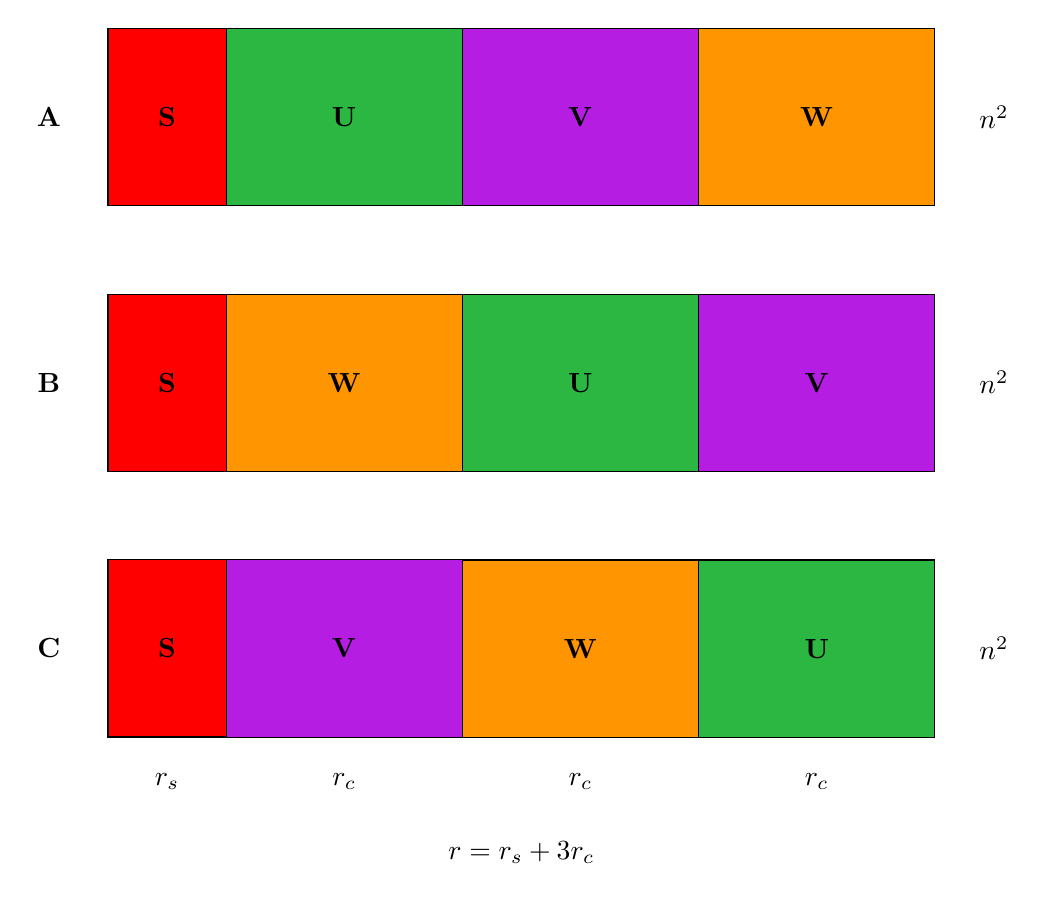
\begin{tikzpicture}[scale=1.5,namenode/.style={scale=1}]
    \def\ix{2} % This modifies the width of the objects
    \def\iy{1.5} % This modifies the height of the objects
    \def\is{1} %
    \def\h{.75}
    \def\corescale{1.75}
    \def\rx{\ix/\corescale}
    \def\ry{\iy/\corescale}
    \def\rz{\is/\corescale}
    
    \coordinate (MiddleS) at (0, 0);
    \draw[fill=red] (MiddleS) rectangle ++ (\is,\iy);
    \node[namenode] at ($(MiddleS) + (0.5*\is, 0.5*\iy)$)  {$\mathbf{S}$};
    \node[namenode] at ($(MiddleS) + (-0.5*\is, 0.5*\iy)$)  {$\mathbf{B}$};
    
    \coordinate (MiddleW) at ($(MiddleS) + (\is,0)$);
    \draw[fill=mycustomorange] (MiddleW) rectangle ++ (\ix,\iy);
    \node[namenode] at ($(MiddleW) + (0.5*\ix, 0.5*\iy)$)  {$\mathbf{W}$};

    \coordinate (MiddleU) at ($(MiddleW) + (\ix,0)$);
    \draw[fill=mycustomgreen] (MiddleU) rectangle ++ (\ix,\iy);
    \node[namenode] at ($(MiddleU) + (0.5*\ix, 0.5*\iy)$)  {$\mathbf{U}$};
    
    \coordinate (MiddleV) at ($(MiddleU) + (\ix,0)$);
    \draw[fill=mycustompurple] (MiddleV) rectangle ++ (\ix,\iy);
    \node[namenode] at ($(MiddleV) + (0.5*\ix, 0.5*\iy)$)  {$\mathbf{V}$};
    \node[namenode] at ($(MiddleV) + (1.25*\ix, 0.5*\iy)$)  {$n^2$};


    \coordinate (TopS) at ($(MiddleS) + (0, \iy + \h)$);
    \draw[fill=red] (TopS) rectangle ++ (\is,\iy);
    \node[namenode] at ($(TopS) + (0.5*\is, 0.5*\iy)$)  {$\mathbf{S}$};
    \node[namenode] at ($(TopS) + (-0.5*\is, 0.5*\iy)$)  {$\mathbf{A}$};

    \coordinate (TopU) at ($(TopS) + (\is,0)$);
    \draw[fill=mycustomgreen] (TopU) rectangle ++ (\ix,\iy);
    \node[namenode] at ($(TopU) + (0.5*\ix, 0.5*\iy)$)  {$\mathbf{U}$};

    \coordinate (TopV) at ($(TopU) + (\ix,0)$);
    \draw[fill=mycustompurple] (TopV) rectangle ++ (\ix,\iy);
    \node[namenode] at ($(TopV) + (0.5*\ix, 0.5*\iy)$)  {$\mathbf{V}$};
    
    \coordinate (TopW) at ($(TopV) + (\ix,0)$);
    \draw[fill=mycustomorange] (TopW) rectangle ++ (\ix,\iy);
    \node[namenode] at ($(TopW) + (0.5*\ix, 0.5*\iy)$)  {$\mathbf{W}$};
    \node[namenode] at ($(TopW) + (1.25*\ix, 0.5*\iy)$)  {$n^2$};


    \coordinate (BottomS) at ($(MiddleS) - (0, \iy + \h)$);
    \draw[fill=red] (BottomS) rectangle ++ (\is,\iy);
    \node[namenode] at ($(BottomS) + (0.5*\is, 0.5*\iy)$)  {$\mathbf{S}$};
    \node[namenode] at ($(BottomS) + (-0.5*\is, 0.5*\iy)$)  {$\mathbf{C}$};
    \node[namenode] at ($(BottomS) + (0.5*\is, -0.25*\iy)$)  {$r_s$};

    \coordinate (BottomV) at ($(BottomS) + (\is,0)$);
    \draw[fill=mycustompurple] (BottomV) rectangle ++ (\ix,\iy);
    \node[namenode] at ($(BottomV) + (0.5*\ix, 0.5*\iy)$)  {$\mathbf{V}$};
    \node[namenode] at ($(BottomV) + (0.5*\ix, -0.25*\iy)$)  {$r_c$};

    \coordinate (BottomW) at ($(BottomV) + (\ix,0)$);
    \draw[fill=mycustomorange] (BottomW) rectangle ++ (\ix,\iy);
    \node[namenode] at ($(BottomW) + (0.5*\ix, 0.5*\iy)$)  {$\mathbf{W}$};
    \node[namenode] at ($(BottomW) + (0.5*\ix, -0.25*\iy)$)  {$r_c$};
    \node[namenode] at ($(\is/2 + 3*\ix/2, -2.15*\iy)$)  {$r = r_s + 3r_c$};
    
    \coordinate (BottomU) at ($(BottomW) + (\ix,0)$);
    \draw[fill=mycustomgreen] (BottomU) rectangle ++ (\ix,\iy);
    \node[namenode] at ($(BottomU) + (0.5*\ix, 0.5*\iy)$)  {$\mathbf{U}$};
    \node[namenode] at ($(BottomU) + (0.5*\ix, -0.25*\iy)$)  {$r_c$};
    \node[namenode] at ($(BottomU) + (1.25*\ix, 0.5*\iy)$)  {$n^2$};
\end{tikzpicture}
    \caption{Cyclic Invariance in a KTensor}
    \label{fig:cyc_inv_matrices}
\end{figure}

\begin{figure}
    \centering
    \begin{tikzpicture}[scale=0.75,namenode/.style={scale=0.75}]
    \def\ix{2} % This modifies the height of the objects
    \def\iy{2} % This modifies the width of the objects
    \def\iz{2.5} %
    \def\r{.25}

    %%%%%%%%%%%%%%%
    %%%    S    %%%
    %%%%%%%%%%%%%%%

    %%%%%%%%% 1st S Component %%%%%%%%%
    % This draws the vertical chicken feet
    \coordinate (S1VLowerLeft) at (0,0);
    \draw[fill=red] (S1VLowerLeft) rectangle ++ (\r,\iy);
    \node[namenode] at ($(S1VLowerLeft)-(0,2*\r)$) {$\mathbf{S}_1$};

    % This draws the horizontal chicken feet
    \coordinate (S1HLowerLeft) at ($(S1VLowerLeft) + (\r,\iy) + (\r,\r)$);
    \draw[fill=red] (S1HLowerLeft) rectangle ++ (\ix,\r);
    \node[namenode] at ($(S1HLowerLeft)+(.5*\iy,-2*\r)$) {$\mathbf{S}_1$};

    % This scopee draws the tp-screen chicken feet
    \begin{scope}[shift={(0,2*\r)},canvas is zx plane at y=\iy,rotate=90]
        \draw[fill=red] (0,\r) rectangle ++ (\r,\iz);
    \end{scope}
    \node[namenode] at ($(S1HLowerLeft)+(.6*\ix,1)$) {$\mathbf{S}_1$};
    
    % S ellipsis
    \coordinate (SEllipsis) at (2*\iy,.75*\ix);
    \node[namenode] at (SEllipsis) {$+ \quad \cdots \quad +$};
    
    %%%%%%%%% last S Component %%%%%%%%%
    % This draws the vertical chicken feet
    \coordinate (SRVLowerLeft) at ($(SEllipsis) + (\iy,-.75*\ix)$);
    \draw[fill=red] (SRVLowerLeft) rectangle ++ (\r,\iy);
    \node[namenode] at ($(SRVLowerLeft)-(0,2*\r)$) {$\mathbf{S}_{r_s}$};

    % This draws the horizontal chicken feet
    \coordinate (SRHLowerLeft) at ($(SRVLowerLeft) + (\r,\iy) + (\r,\r)$);
    \draw[fill=red] (SRHLowerLeft) rectangle ++ (\ix,\r);
    \node[namenode] at ($(SRHLowerLeft)+(.5*\iy,-2*\r)$) {$\mathbf{S}_{r_s}$};
    
        % This scopee draws the tp-screen chicken feet
    \begin{scope}[shift={(3*\iy,2*\r)},canvas is zx plane at y=\iy,rotate=90]
        \draw[fill=red] (0,\r) rectangle ++ (\r,\iz);
    \end{scope}
    \node[namenode] at ($(SRHLowerLeft)+(.6*\ix,1)$) {$\mathbf{S}_{r_s}$};

    %%%%%%%%%%%%%%%%
    %%% Cyclic 1 %%%
    %%%%%%%%%%%%%%%%
    
    % top sum
    \coordinate (TopSum) at (4.5*\iy,.75*\ix);
    \node[namenode] at (TopSum) {$+ $};

    %%%%%%%%% 1st Cyclic 1 Component %%%%%%%%%
    % This draws the vertical chicken feet
    \coordinate (U1VLowerLeft) at ($(TopSum) - (0,0.75*\iy) + (0.75,0)$);
    \draw[fill=mycustomgreen] (U1VLowerLeft) rectangle ++ (\r,\iy);
    \node[namenode] at ($(U1VLowerLeft)-(0,2*\r)$) {$\mathbf{U}_1$};

    % This draws the horizontal chicken feet
    \coordinate (W1HLowerLeft) at ($(U1VLowerLeft) + (\r,\iy) + (\r,\r)$);
    \draw[fill=mycustomorange] (W1HLowerLeft) rectangle ++ (\ix,\r);
    \node[namenode] at ($(W1HLowerLeft)+(.5*\iy,-2*\r)$) {$\mathbf{W}_1$};

    % This scopee draws the to-screen chicken feet
    \begin{scope}[shift={(4.875*\iy,2*\r)},canvas is zx plane at y=\iy,rotate=90]
        \draw[fill=mycustompurple] (0,\r) rectangle ++ (\r,\iz);
    \end{scope}
    \node[namenode] at ($(W1HLowerLeft)+(.6*\ix,1)$) {$\mathbf{V}_1$};
    
    % top ellipsis
    \coordinate (TopEllipsis) at (6.875*\iy,.75*\ix);
    \node[namenode] at (TopEllipsis) {$+ \quad \cdots \quad +$};
    
    %%%%%%%%% last Cyclic 1 Component %%%%%%%%%
    % This draws the vertical chicken feet
    \coordinate (URVLowerLeft) at ($(TopEllipsis) + (\iy,-.75*\ix)$);
    \draw[fill=mycustomgreen] (URVLowerLeft) rectangle ++ (\r,\iy);
    \node[namenode] at ($(URVLowerLeft)-(0,2*\r)$) {$\mathbf{U}_{r_c}$};

    % This draws the horizontal chicken feet
    \coordinate (WRHLowerLeft) at ($(URVLowerLeft) + (\r,\iy) + (\r,\r)$);
    \draw[fill=mycustomorange] (WRHLowerLeft) rectangle ++ (\ix,\r);
    \node[namenode] at ($(WRHLowerLeft)+(.5*\iy,-2*\r)$) {$\mathbf{W}_{r_c}$};

    % This scopee draws the to-screen chicken feet
    \begin{scope}[shift={(7.875*\iy,2*\r)},canvas is zx plane at y=\iy,rotate=90]
        \draw[fill=mycustompurple] (0,\r) rectangle ++ (\r,\iz);
    \end{scope}
    \node[namenode] at ($(WRHLowerLeft)+(.6*\ix,1)$) {$\mathbf{V}_{r_c}$};

    %%%%%%%%%%%%%%%%
    %%% Cyclic 2 %%%
    %%%%%%%%%%%%%%%%

    % middle sum
    \coordinate (MiddleSum) at ($(TopSum) + (0, -17*\r)$);
    \node[namenode] at (MiddleSum) {$+ $};

    %%%%%%%%% 1st Cyclic 2 Component %%%%%%%%%
    % This draws the vertical chicken feet
    \coordinate (V1VLowerLeft) at ($(MiddleSum) - (0,0.75*\iy) + (0.75,0)$);
    \draw[fill=mycustompurple] (V1VLowerLeft) rectangle ++ (\r,\iy);
    \node[namenode] at ($(V1VLowerLeft)-(0,2*\r)$) {$\mathbf{V}_1$};

    % This draws the horizontal chicken feet
    \coordinate (U1HLowerLeft) at ($(V1VLowerLeft) + (\r,\iy) + (\r,\r)$);
    \draw[fill=mycustomgreen] (U1HLowerLeft) rectangle ++ (\ix,\r);
    \node[namenode] at ($(U1HLowerLeft)+(.5*\iy,-2*\r)$) {$\mathbf{U}_1$};

    % This scopee draws the tp-screen chicken feet
    \begin{scope}[shift={(4.875*\iy,-15*\r)},canvas is zx plane at y=\iy,rotate=90]
        \draw[fill=mycustomorange] (0,\r) rectangle ++ (\r,\iz);
    \end{scope}
    \node[namenode] at ($(U1HLowerLeft)+(.6*\ix,1)$) {$\mathbf{W}_1$};
    
    % middle ellipsis
    \coordinate (MiddleEllipsis) at ($(MiddleSum) + (4.75, 0)$);
    \node[namenode] at (MiddleEllipsis) {$+ \quad \cdots \quad +$};
    
    %%%%%%%%% last Cyclic 2 Component %%%%%%%%%
    % This draws the vertical chicken feet
    \coordinate (VRVLowerLeft) at ($(MiddleEllipsis) + (\iy,-.75*\ix)$);
    \draw[fill=mycustompurple] (VRVLowerLeft) rectangle ++ (\r,\iy);
    \node[namenode] at ($(VRVLowerLeft)-(0,2*\r)$) {$\mathbf{V}_{r_c}$};

    % This draws the horizontal chicken feet
    \coordinate (URHLowerLeft) at ($(VRVLowerLeft) + (\r,\iy) + (\r,\r)$);
    \draw[fill=mycustomgreen] (URHLowerLeft) rectangle ++ (\ix,\r);
    \node[namenode] at ($(URHLowerLeft)+(.5*\iy,-2*\r)$) {$\mathbf{U}_{r_c}$};
    
    % This scopee draws the tp-screen chicken feet
    \begin{scope}[shift={(7.875*\iy,-15*\r)},canvas is zx plane at y=\iy,rotate=90]
        \draw[fill=mycustomorange] (0,\r) rectangle ++ (\r,\iz);
    \end{scope}
    \node[namenode] at ($(URHLowerLeft)+(.6*\ix,1)$) {$\mathbf{W}_{r_c}$};

    %%%%%%%%%%%%%%%%
    %%% Cyclic 3 %%%
    %%%%%%%%%%%%%%%%
    
    % bottom sum
    \coordinate (BottomSum) at ($(MiddleSum) + (0, -17*\r)$);
    \node[namenode] at (BottomSum) {$+ $};

    %%%%%%%%% 1st Cyclic 3 Component %%%%%%%%%
    % This draws the vertical chicken feet
    \coordinate (W1VLowerLeft) at ($(BottomSum) - (0,0.75*\iy) + (0.75,0)$);
    \draw[fill=mycustomorange] (W1VLowerLeft) rectangle ++ (\r,\iy);
    \node[namenode] at ($(W1VLowerLeft)-(0,2*\r)$) {$\mathbf{W}_1$};

    % This draws the horizontal chicken feet
    \coordinate (V1HLowerLeft) at ($(W1VLowerLeft) + (\r,\iy) + (\r,\r)$);
    \draw[fill=mycustompurple] (V1HLowerLeft) rectangle ++ (\ix,\r);
    \node[namenode] at ($(V1HLowerLeft)+(.5*\iy,-2*\r)$) {$\mathbf{V}_1$};

    % This scopee draws the tp-screen chicken feet
    \begin{scope}[shift={(4.875*\iy,-2.125*15*\r)},canvas is zx plane at y=\iy,rotate=90]
        \draw[fill=mycustomgreen] (0,\r) rectangle ++ (\r,\iz);
    \end{scope}
    \node[namenode] at ($(V1HLowerLeft)+(.6*\ix,1)$) {$\mathbf{U}_1$};
    
    % bottom ellipsis
    \coordinate (MiddleEllipsis) at ($(BottomSum) + (4.75, 0)$);
    \node[namenode] at (MiddleEllipsis) {$+ \quad \cdots \quad +$};
    
    %%%%%%%%% last Cyclic 3 Component %%%%%%%%%
    % This draws the vertical chicken feet
    \coordinate (WRVLowerLeft) at ($(MiddleEllipsis) + (\iy,-.75*\ix)$);
    \draw[fill=mycustomorange] (WRVLowerLeft) rectangle ++ (\r,\iy);
    \node[namenode] at ($(WRVLowerLeft)-(0,2*\r)$) {$\mathbf{W}_{r_c}$};

    % This draws the horizontal chicken feet
    \coordinate (VRHLowerLeft) at ($(WRVLowerLeft) + (\r,\iy) + (\r,\r)$);
    \draw[fill=mycustompurple] (VRHLowerLeft) rectangle ++ (\ix,\r);
    \node[namenode] at ($(VRHLowerLeft)+(.5*\iy,-2*\r)$) {$\mathbf{V}_{r_c}$};

    % This scopee draws the tp-screen chicken feet
    \begin{scope}[shift={(7.875*\iy,-2.125*15*\r)},canvas is zx plane at y=\iy,rotate=90]
        \draw[fill=mycustomgreen] (0,\r) rectangle ++ (\r,\iz);
    \end{scope}
    \node[namenode] at ($(VRHLowerLeft)+(.6*\ix,1)$) {$\mathbf{U}_{r_c}$};
\end{tikzpicture}

    \caption{CP Decomposition Diagram with Cyclic Invariant Structure}
    \label{fig:cyc_inv_cp}
\end{figure}


\newpage
\subsection{Adapting CP\_DGN to Cyclic Invariance} \label{Adapting CP-DGN to Cyclic Invariance}

    We must now adapt \Cref{sec:Cyclic Invariant Matrix Multiplication
    Algorithms} to our cyclic invariance structure. Now we have the imposed
    structure on any CP Decomposition of the matrix multiplication tensor. 

    \begin{equation*}
        \begin{array}{rcl}
            \mathbf{A} = [\begin{array}{cccc} \mathbf S & \mathbf U & \mathbf V & \mathbf W \end{array}]\\
            \mathbf{B} = [\begin{array}{cccc} \mathbf S & \mathbf W & \mathbf U & \mathbf V \end{array}]\\
            \mathbf{C} = [\begin{array}{cccc} \mathbf S & \mathbf V & \mathbf W & \mathbf U \end{array}]
        \end{array}
    \end{equation*}

    That means \Cref{eq:cp_least_squares} becomes \Cref{eq:ci_cp_least_squares}
    in accordance with \Cref{fig:cyc_inv_cp}. 

    \begin{equation} \label{eq:ci_cp_least_squares}
        f(v) = \frac{1}{2} \sum_{i}^m \sum_{j}^n \sum_{k}^p \left( x_{ijk} - \sum_{q}^{r_s} s_{iq}s_{jq}s_{kq} - \sum_{l}^{r_c} (u_{il}v_{jl}w_{kl} + w_{il}u_{jl}v_{kl} + v_{il}w_{jl}u_{kl}) \right)^2
    \end{equation}

    In order for that to be the case, we must change our $\mathbf{v}$ such that

    \begin{equation*}
        \mathbf{v} = \text{vec}
        \left(
        \left[
            \begin{array}{c}
                \mathbf{S} \\
                \mathbf{U} \\
                \mathbf{V} \\
                \mathbf{W}
            \end{array}
        \right]
        \right) = 
        \left[
            \begin{array}{c}
                \text{vec}(\mathbf{S}) \\
                \text{vec}(\mathbf{U}) \\
                \text{vec}(\mathbf{V}) \\
                \text{vec}(\mathbf{W})
            \end{array}
        \right]
        \in \mathbb{R}^{nr}
    \end{equation*}

    The Gradient becomes

    \begin{equation}
        \nabla f =
        \left[
        \begin{array}{c}
                \mathsf{vec}(\frac{\partial f}{\partial \mathbf{S}})\\
                \mathsf{vec}(\frac{\partial f}{\partial \mathbf{U}})\\
                \mathsf{vec}(\frac{\partial f}{\partial \mathbf{V}})\\
                \mathsf{vec}(\frac{\partial f}{\partial \mathbf{W}})
        \end{array}
        \right]
        \in \mathbb{R}^{(m+n+p)r}
    \end{equation}

    Where each partial derivative is defined as:

    \begin{equation}
        \begin{array}{rcl}
            \frac{\partial f}{\partial \mathbf{S}} & = & \scriptstyle 3 \mathbf{\cdot \bigl(S\left(S^\intercal S\ast S^\intercal S\right) + U\left(V^\intercal S\ast W^\intercal S\right) + V\left(U^\intercal S\ast W^\intercal S\right) + W\left(U^\intercal S\ast V^\intercal S\right)}\\ 
            & & \scriptstyle - \mathbf{(X_{(1)} + X_{(2)} + X_{(3)})(S\odot S)}\bigl) \\

            \frac{\partial f}{\partial \mathbf{U}} & = & \scriptstyle 3\mathbf{\cdot \bigl(S\left(S^\intercal V\ast S^\intercal W\right) + U\left(V^\intercal V\ast W^\intercal W\right) + V\left(W^\intercal V\ast U^\intercal W\right) + W\left(U^\intercal V\ast V^\intercal W\right)\bigl)}\\ 
            & & \scriptstyle - \mathbf{X_{(1)}(V\odot W) - X_{(2)}(W\odot V) - X_{(3)}(V\odot W)} \\

            \frac{\partial f}{\partial \mathbf{V}} & = & \scriptstyle 3\mathbf{\cdot \bigl(S\left(S^\intercal U\ast S^\intercal W\right) + U\left(W^\intercal U\ast V^\intercal W\right) + V\left(U^\intercal U\ast W^\intercal W\right) + W\left(V^\intercal U\ast U^\intercal W\right)\bigl)}\\ 
            & & \scriptstyle - \mathbf{X_{(1)}(W\odot U) - X_{(2)}(U\odot W) - X_{(3)}(W\odot U)} \\

            \frac{\partial f}{\partial \mathbf{W}} & = & \scriptstyle 3\mathbf{\cdot \bigl(S\left(S^\intercal U\ast S^\intercal V\right) + U\left(V^\intercal U\ast W^\intercal V\right) + V\left(W^\intercal U\ast U^\intercal V\right) + W\left(U^\intercal U\ast V^\intercal V\right)\bigl)}\\ 
            & & \scriptstyle - \mathbf{X_{(1)}(U\odot V) - X_{(2)}(V\odot U) - X_{(3)}(U\odot V)}
        \end{array}
        \label{eq:ci_cp_dgn_partials}
    \end{equation}

    Similarly, our jacobian becomes

    \begin{equation} \label{eq:ci_cp_dgn_jacobian}
        \mathbf{J} = [\mathbf{J}_\mathbf{S} + \mathbf{J}_\mathbf{U} + \mathbf{J}_\mathbf{V} + \mathbf{J}_\mathbf{W}] \in \mathbb{R}^{n^3\times nr}
    \end{equation}
    
    Where
    
    \begin{equation}
        \begin{array}{rcl}
                \mathbf{J}_\mathbf{S} & = \mathbf{(S\odot S)} \otimes \mathbf{I} + \mathbf{\Pi}_2^\intercal\cdot \mathbf{(S\odot S)} \otimes \mathbf{I} + \mathbf{\Pi}_3^\intercal\cdot \mathbf{(S\odot S)} \otimes \mathbf{I}\\
                \mathbf{J}_\mathbf{U} & = \mathbf{(V\odot W)} \otimes \mathbf{I} + \mathbf{\Pi}_2^\intercal\cdot \mathbf{(W\odot V)} \otimes \mathbf{I} + \mathbf{\Pi}_3^\intercal\cdot \mathbf{(V\odot W)} \otimes \mathbf{I}\\
                \mathbf{J}_\mathbf{V} & = \mathbf{(W\odot U)} \otimes \mathbf{I} + \mathbf{\Pi}_2^\intercal\cdot \mathbf{(U\odot W)} \otimes \mathbf{I} + \mathbf{\Pi}_3^\intercal\cdot \mathbf{(W\odot U)} \otimes \mathbf{I}\\
                \mathbf{J}_\mathbf{V} & = \mathbf{(U\odot V)} \otimes \mathbf{I} + \mathbf{\Pi}_2^\intercal\cdot \mathbf{(V\odot U)} \otimes \mathbf{I} + \mathbf{\Pi}_3^\intercal\cdot \mathbf{(U\odot V)} \otimes \mathbf{I}
        \end{array}
        \label{eq:ci_cp_dgn_jacobians}
    \end{equation}

    However, just like in \Cref{sec:Damped Gauss Newton Optimization for CP
    Decompositions}, we don't care as much about the explicit jacobian as we do
    about how to apply $\mathbf{J^\intercal J}$ to a vector. 

    \begin{equation}
        \mathbf{J^\intercal J} \cdot \text{vec}(\mathbf{K}) = 
        \left[
        \begin{array}{cccc}
            \mathbf{J_S^\intercal J_S} & \mathbf{J_S^\intercal J_U} & \mathbf{J_S^\intercal J_V} & \mathbf{J_S^\intercal J_W} \\
            \mathbf{J_U^\intercal J_S} & \mathbf{J_U^\intercal J_U} & \mathbf{J_U^\intercal J_V} & \mathbf{J_U^\intercal J_W} \\
            \mathbf{J_V^\intercal J_S} & \mathbf{J_V^\intercal J_U} & \mathbf{J_V^\intercal J_V} & \mathbf{J_V^\intercal J_W} \\
            \mathbf{J_W^\intercal J_S} & \mathbf{J_W^\intercal J_U} & \mathbf{J_W^\intercal J_V} & \mathbf{J_W^\intercal J_W}
        \end{array}
        \right]
        \left[
        \begin{array}{c}
            \text{vec}(\mathbf{K_S}) \\
            \text{vec}(\mathbf{K_U}) \\
            \text{vec}(\mathbf{K_V}) \\
            \text{vec}(\mathbf{K_W})
        \end{array}
        \right]
    \end{equation}

    The equations for each entry of the above matrix-vector product can be found below:

    \newpage
    \begin{equation*}
        \begin{array}{ccc}
                \mathbf{J_S^\intercal J_S \text{vec}(K_s)} & = & \scriptstyle 3\cdot \text{vec}\bigl(\mathbf{K_S(S^\intercal S)\ast (S^\intercal S) + 2\cdot S(K_S^\intercal S)\ast (S^\intercal S)}\bigl) \\
                \mathbf{J_S^\intercal J_U \text{vec}(K_u)} & = & \scriptstyle 3\cdot \text{vec}\bigl(\mathbf{K_U(V^\intercal S)\ast (W^\intercal S) + V(K_U^\intercal S)\ast (W^\intercal S) + W(K_U^\intercal S)\ast (V^\intercal S)}\bigl) \\
                \mathbf{J_S^\intercal J_V \text{vec}(K_v)} & = & \scriptstyle 3\cdot \text{vec}\bigl(\mathbf{K_V(U^\intercal S)\ast (W^\intercal S) + U(K_V^\intercal S)\ast (W^\intercal S) + W(K_V^\intercal S)\ast (U^\intercal S)}\bigl) \\
                \mathbf{J_S^\intercal J_W \text{vec}(K_w)} & = & \scriptstyle 3\cdot \text{vec}\bigl(\mathbf{K_W(U^\intercal S)\ast (V^\intercal S) + U(K_W^\intercal S)\ast (V^\intercal S) + V(K_W^\intercal S)\ast (U^\intercal S)}\bigl) \\ \\
                \mathbf{J_U^\intercal J_S \text{vec}(K_s)} & = & \scriptstyle 3\cdot \text{vec}\bigl(\mathbf{K_S(S^\intercal V)\ast (S^\intercal W) + S\bigl((K_S^\intercal W)\ast (S^\intercal V) + (K_S^\intercal V)\ast (S^\intercal W)\bigl)}\bigl) \\
                \mathbf{J_U^\intercal J_U \text{vec}(K_u)} & = & \scriptstyle 3\cdot \text{vec}\bigl(\mathbf{K_U(V^\intercal V)\ast (W^\intercal W) + V(K_U^\intercal W)\ast (W^\intercal V) + W(K_U^\intercal V)\ast (V^\intercal W)}\bigl) \\
                \mathbf{J_U^\intercal J_V \text{vec}(K_v)} & = & \scriptstyle 3\cdot \text{vec}\bigl(\mathbf{K_V(W^\intercal V)\ast (U^\intercal W) + W(K_V^\intercal W)\ast (U^\intercal V) + U(K_V^\intercal V)\ast (W^\intercal W)}\bigl) \\
                \mathbf{J_U^\intercal J_W \text{vec}(K_w)} & = & \scriptstyle 3\cdot \text{vec}\bigl(\mathbf{K_W(U^\intercal V)\ast (V^\intercal W) + U(K_W^\intercal W)\ast (V^\intercal V) + V(K_W^\intercal V)\ast (U^\intercal W)}\bigl) \\ \\
                \mathbf{J_V^\intercal J_S \text{vec}(K_s)} & = & \scriptstyle 3\cdot \text{vec}\bigl(\mathbf{K_S(S^\intercal U)\ast (S^\intercal W) + S\bigl((K_S^\intercal U)\ast (S^\intercal W) + (K_S^\intercal W)\ast (S^\intercal U)\bigl)}\bigl) \\
                \mathbf{J_V^\intercal J_U \text{vec}(K_u)} & = & \scriptstyle 3\cdot \text{vec}\bigl(\mathbf{K_U(V^\intercal W)\ast (W^\intercal U) + V(K_U^\intercal U)\ast (W^\intercal W) + W(K_U^\intercal W)\ast (V^\intercal U)}\bigl) \\
                \mathbf{J_V^\intercal J_V \text{vec}(K_v)} & = & \scriptstyle 3\cdot \text{vec}\bigl(\mathbf{K_V(W^\intercal W)\ast (U^\intercal U) + W(K_V^\intercal U)\ast (U^\intercal W) + U(K_V^\intercal W)\ast (W^\intercal U)}\bigl) \\
                \mathbf{J_V^\intercal J_W \text{vec}(K_w)} & = & \scriptstyle 3\cdot \text{vec}\bigl(\mathbf{K_W(U^\intercal W)\ast (V^\intercal U) + U(K_W^\intercal U)\ast (V^\intercal W) + V(K_W^\intercal W)\ast (U^\intercal U)}\bigl) \\ \\
                \mathbf{J_W^\intercal J_S \text{vec}(K_s)} & = & \scriptstyle 3\cdot \text{vec}\bigl(\mathbf{K_S(S^\intercal U)\ast (S^\intercal V) + S\bigl((K_S^\intercal U)\ast (S^\intercal V) + (K_S^\intercal V)\ast (S^\intercal U)\bigl)}\bigl) \\
                \mathbf{J_W^\intercal J_U \text{vec}(K_u)} & = & \scriptstyle 3\cdot \text{vec}\bigl(\mathbf{K_U(V^\intercal U)\ast (W^\intercal V) + V(K_U^\intercal V)\ast (W^\intercal U) + W(K_U^\intercal U)\ast (V^\intercal V)}\bigl) \\
                \mathbf{J_W^\intercal J_V \text{vec}(K_v)} & = & \scriptstyle 3\cdot \text{vec}\bigl(\mathbf{K_V(W^\intercal W)\ast (U^\intercal V) + W(K_V^\intercal V)\ast (U^\intercal U) + U(K_V^\intercal U)\ast (W^\intercal V)}\bigl) \\
                \mathbf{J_W^\intercal J_W \text{vec}(K_w)} & = & \scriptstyle 3\cdot \text{vec}\bigl(\mathbf{K_W(U^\intercal U)\ast (V^\intercal V) + U(K_W^\intercal V)\ast (V^\intercal U) + V(K_W^\intercal U)\ast (U^\intercal V)}\bigl) \\
        \end{array}
    \end{equation*}

    Then, we reach our algorithm
    \begin{algorithm}
        \caption{Cyclic Invariant CP Damped Gauss-Newton}
        \label{alg:Mod-CP-DGN}
        \begin{algorithmic}
            \State{\textbf{Input:} Matrix Multiplication Tensor $\mathcal{M}$,}
            \State{\hspace{3.25em} CP Tensor Rank $r$,}
            \State{\hspace{3.25em} Damping Parameter $\lambda \in \mathbb{R}$,}
            \State{\hspace{3.25em} Convergence Tolerance $\epsilon > 0$}
            
            \State \textbf{Output:} CP Tensor $\mathcal{K}$
            \Function{DGN}{$\mathcal{M}, r, \lambda, \epsilon$}
                \State{Initialize K and K\_prev to be a cell of length 4 with the first entry being of $n^2 \times r_s$ and the remaining three $n^2 \times r_c$ matrices}

                \For{$i = 1:MaxIters$}
                    \State{f $\longleftarrow \frac{1}{2} \|\mathcal{M} - \mathbf{\llbracket S, S, S\rrbracket - \llbracket U, V, W\rrbracket - \llbracket W, U, V\rrbracket - \llbracket V, W, U\rrbracket} \| $}
                    \State{$\nabla \mathbf{f} \longleftarrow [\text{vec} \left( \frac{\partial f}{\partial \mathbf S}\right) \text{vec} \left( \frac{\partial f}{\partial \mathbf U}\right) \text{vec} \left( \frac{\partial f}{\partial \mathbf V}\right) \text{vec} \left( \frac{\partial f}{\partial \mathbf W}\right)]^T$} 
                    \State{$S \longleftarrow \text{Solution to } (\textbf{J}^T\textbf{J} + \lambda I)\mathbf{K} = -\nabla \mathbf{f}$}
                    \While{\textit{Goldstein Conditions Are Satisfied}}
                        \State{K $\longleftarrow$ K\_prev + $\alpha S$}
                        \State{f $_{new}\longleftarrow$ Compute Function Value}
                        \State{$\alpha \longleftarrow \alpha / 2$}
                    \EndWhile{}
                    \If{f - f $_{new} < \epsilon$}
                        \State{\textbf{break}}
                    \EndIf{}
                \EndFor{}
            \EndFunction
        \end{algorithmic}
    \end{algorithm}

\newpage
\section{Further Structure in Matrix Multiplication Algorithms} \label{sec:Further Structure in Matrix Multiplication Algorithms}

\JP{This is ongoing work. Essentially, we are searching for additional
structure in the solutions we have found. I will try to summarize the main ideas
in the talk as well as in this section before I graduate, but realistic the
precise writing of this section won't be in its full version before I graduate}





        \newpage





    %%%%%%%%%%%%%%%%%%%%%%%%%%%%%%%%%%%%%%%%%%
    %% Chapter 3 - The Tucker Decomposition %%
    %%%%%%%%%%%%%%%%%%%%%%%%%%%%%%%%%%%%%%%%%%
    \chapter{\textbf{The Tucker Decomposition}}
        %!TEX root = ../../main.tex

The rank of a Tucker decomposition, given by the size of $\mathcal{G}$, directly
impacts the amount of compression, so the choice of rank is consequential. If
the decomposition's ranks are large, then great accuracy is achieved at the cost
of poor compression. If the decomposition's ranks are small, then great
compression is achieved at the cost of poor accuracy. This is known as the
tensor decomposition trade-off as seen in
\Cref{fig:tensor_decomposition_trade_off}. It is applied to all forms of
decompositions, but it is specially relevant here. 

\begin{figure}[ht!]
    \centering
    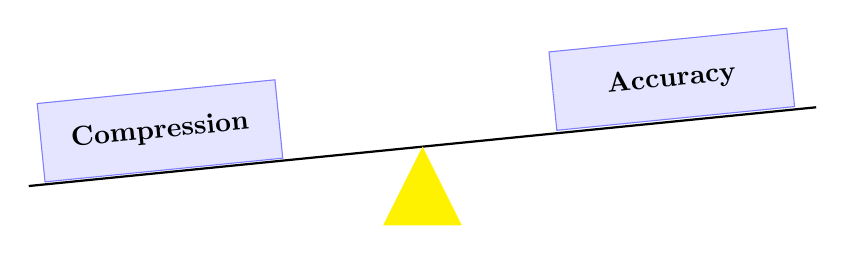
\begin{tikzpicture}

    % Seesaw beam (tilted from -5 to 5)
    \draw[thick] (-5,-0.5) -- (5,0.5);
    
    % Fulcrum (yellow triangle)
    \fill[yellow] (0,0) -- (-0.5,-1) -- (0.5,-1) -- cycle;

    % Rotation angle to match the beam tilt
    \def\tiltangle{5.7} % positive to match the upward slope from left to right

    % Left box - Compression (rotated to match beam angle)
    \node[draw=blue!50, fill=blue!10, text width=2.8cm, minimum height=1cm,
          align=center, anchor=south west, rotate=\tiltangle] at (-4.8,-0.455) {\textbf{Compression}};
    
    % Right box - Accuracy (rotated to match beam angle)
    \node[draw=blue!50, fill=blue!10, text width=2.8cm, minimum height=1cm,
          align=center, anchor=south west, rotate=\tiltangle] at (1.7,0.2) {\textbf{Accuracy}};
    
    
\end{tikzpicture}
    \caption{The Tensor Decomposition Trade-Off}
    \label{fig:tensor_decomposition_trade_off}
\end{figure}

To know compression beforehand, we specify the size of the core tensor
$\mathcal{G}$. In the 3-way case, we specify the array of ranks $\mathbf{r} =
[q, r, s]$, or in the $d$-way case, $\mathbf{r} = [r_1, \hdots, r_d]$. Because
we know the ranks beforehand, this is called the \textbf{rank-specified}
formulation, and with it, we also know the compression ratio before hand as seen
in \Cref{eq:compression_ratio} for the 3-way case. In this formulation, we
cannot say in advance what the accuracy will be.

\begin{equation} \label{eq:compression_ratio}
    \frac{mnp}{qrs + qm + nr + sp} \approx \frac{mnp}{qrs}
\end{equation}

To know accuracy beforehand, we specify the maximum relative error threshold
$\epsilon$ of the tucker approximation. The 3-way case of the relative error can
be seen in \Cref{eq:rel_error}. This is called the \textbf{error-specified}
formulation, where we cannot say in advance what the compression will be. 

\begin{equation} \label{eq:rel_error}
    \frac{\| \mathcal{X} - \llbracket \mathcal{G}; \mathbf{U, V, W} \rrbracket \|}{\|\mathcal{X}\|} \leq \epsilon
\end{equation}

We now go on a journey to understand two of the main Tucker Decomposition
algorithms; STHOSVD and HOOI. STHOSVD is the more popular of the two for many
reasons, but one of them is that the algorithm works in both rank- and
error-specified formulation whereas HOOI, on the other hand, can only work in
the rank-specified formulation. 


\section{Tucker Algorithms} \label{sec:Tucker Algorithms}
    %!TEX root = ../../main.tex

Recall from \Cref{sec:Tucker Tensors and The Tucker Decomposition} that a Tucker
decomposition of a tensor $\mathcal{X}\in \mathbb{R}^{n_1\times \cdots \times
n_d}$ approximates $\mathcal{X}$ as a product of a core tensor $\mathcal{G} \in
\mathbb{R}^{r_1 \cdots r_d}$ and factor matrices $\mathbf{U}_j \in
\mathbb{R}^{n_k\times r_k} \forall k \in [d]$ where $\mathcal{X} \approx
\mathcal{\hat{X}} = \mathcal{G} \times_1 \mathbf{U}_1 \cdots \times
\mathbf{U}_d$. The optimal rank-$\mathbf{r}$ Tucker decomposition of
$\mathcal{X}$ can be expressed as a solution to the rank-specified optimization problem

\begin{equation}\label{eq:tuckeropt-rank}
    \begin{aligned}
        \min \quad & \| \mathcal{X} - (\mathcal{G} \times_1 \mathbf{U}_1 \cdots \times \mathbf{U}_d)\| \\ 
        \text{subject to } &\mathcal{G} \in \mathbb{R}^{r_1\times \cdots \times r_d}, \mathbf{U}_{k} \in \mathbb{R}^{n_k\times r_k} \forall k\in [d].
    \end{aligned}
\end{equation}

Alternatively, the error-specified formulation of the Tucker approximation
problem is given as

\begin{equation}\label{eq:tuckeropt-err}
    \begin{aligned}
        \min \quad & \prod_{j=1}^d r_j + \sum_{j=1}^d n_jr_j & \\ 
        \text{subject to } &\mathcal{G} \in \mathbf{R}^{r_1\times \cdots r_d}, \mathbf{U}_{j} \in \mathbb{R}^{n_k\times r_k} \forall k\in [d] \\
        \text{and}\quad  & \| \mathcal{X} - (\mathcal{G} \times_1 \mathbf{U}_1 \cdots \times \mathbf{U}_d) \| \leq \epsilon \|\mathcal{X}\|.
    \end{aligned}
\end{equation}

\subsection{STHOSVD} \label{sec:sthosvd} 

    We start with the state-of-the art algorithm that is capable of performing
    both rank-specified and error-specified formulations. \Cref{alg:STHOSVD}
    showcases the $d$-way construction of the STHOSVD algorithm. This method
    approximately solves either \cref{eq:tuckeropt-rank} or
    \cref{eq:tuckeropt-err} by unfolding the $k^\text{th}$ mode of the input
    tensor, computing its leaft leading singular vectors (LLSV), and then
    performing a TTM with the result to truncate the $k^\text{th}$ mode of rank
    $r_k$. Once all factor matrices have been computed, the truncated tensor has
    rank $\mathbf{r}$.

    A relative error error of $\epsilon$ can be achieved by selecting $r_k$ in
    the LLSV computation such that \(\sum_{i=r_k+1}^{n_k}\varSigma_i^2 \leq
    \epsilon^2 \|\mathcal{X}\|^2/d\), where $\varSigma_i$ is the $i^\text{th}$ largest
    singular value of the $j^\text{th}$ unfolding, see \cite{BK25} for more
    details. There are several algorithms one could choose in line
    \ref{line:sthosvd_llsv} to compute $\mathbf{U}_k$. We assume that such
    computation is performed via the eigenvalue decomposition (EVD) of the Gram
    matrix $\mathbf{G}_{(k)}\mathbf{G}_{(k)}$. 

    \begin{algorithm}
        \caption{STHOSVD}
        \label{alg:STHOSVD}
        \begin{algorithmic}
            \State{\textbf{Input:} Tensor $\mathcal{X} \in \mathbb{R}^{n_1 \times \cdots \times n_d}$} % \vspace{-0.75em}}
            \State{\hspace{3.25em} Ranks \textbf{R} $ = r_1, \dots, r_d$ \textbf{OR} relative error tolerance $\epsilon > 0$} % \vspace{-0.75em}}
            
            \State{\textbf{Output:} TTensor $\mathcal{T}$ of ranks \textbf{R} with $\mathcal{T \approx X}$ \textbf{OR} E{\footnotesize \text{RR}} $\equiv ||\mathcal{X - T}|| \leq \epsilon ||\mathcal{X}||$}
            \Function{STHOSVD}{$\mathcal{X}$, \textbf{R} or $\epsilon$}
                \State{\textbf{if} $\epsilon$ is defined \textbf{then} $\bar{\epsilon} \gets (\epsilon / \sqrt{d})\cdot||\mathcal{X}||$}
                \State{$\mathcal{G \gets X}$}
                \For{$k = 1, \dots, d$}
                    \State{$[U_k, \epsilon_k] \gets \textcolor{blue}{LLSV}(G_{(k)}, r_k \text{ or } \bar{\epsilon})$}\label{line:sthosvd_llsv} \Comment{$r_k$ leading left sing. vectors of residual} 
                    \State{$\mathcal{G} \gets \mathcal{G \times_k} U^\intercal_k$}\label{line:sthosvd_ttm} \Comment{compress in mode $k$}
                \EndFor{}
                \vspace{10pt}
                \State{E{\footnotesize \text{RR}} $\gets \displaystyle \sqrt{\sum_{k=1}^d \epsilon_k^2}$} \Comment{equivalent to $||\mathcal{X - T}||$}
                \vspace{10pt}
                \State{\textbf{return} [$\mathcal{G}, U_{1:d}$, E{\footnotesize \text{RR}}]} \Comment{$\mathcal{T \equiv \{G; \textit{$U_{1:d}$}\}}$}
            \EndFunction
        \end{algorithmic}
    \end{algorithm}

\subsection{Classic HOOI} \label{sec:Classic HOOI} 

    Our protagonist is given in \cref{alg:Classic-HOOI} and is an alternative
    method for solving the rank-specified formulation of the Tucker
    approximation problem
    \cite{kroonenberg1980principal,de2000best,kapteyn1986approach}. HOOI is a
    block coordinate descent method and so it requires initial factor matrices.
    Historically, the output factor matrices of STHOSVD have been used as input
    factor matrices for the HOOI algorithm, as the latter has often been as an
    aditional algorithm to just cheaply clean up the error. However, random
    factor matrices can be used and generally no more than two iterations are
    requireed to get a good approximation, often only one iteration is enough to
    get a descent one. 

    HOOI iteratively updates each factor matrix by performing a TTM with all but
    the $k^\text{th}$ factor matrix to obtain an intermediate tensor
    $\mathcal{Y}$ and computing the LLSV of $\mathbf{Y}_{(k)}$. The core tensor
    $\mathcal G$ can be computed oce, at the end, or at the end of every
    iteration in order to computate a per-iteration approximation error. 

    \begin{algorithm}
        \caption{HOOI}
        \label{alg:Classic-HOOI}
        \begin{algorithmic}
            \State{\textbf{Input:} Tensor $\mathcal{X} \in \mathbb{R}^{n_1 \times \cdots \times n_d}$}
            \State{\hspace{3.25em} Either Ranks \textbf{R} $ = r_1, \dots, r_d$}
            \State{\hspace{3.25em} Maximum Number of Iterations}
            
            \State{\textbf{Output:} TTensor $\mathcal{T}$ of ranks \textbf{R} with $\mathcal{T \approx X}$}
            \Function{HOOI}{$\mathcal{X}$, \textbf{R} or $\epsilon$}
                \State{Initialize factor matrices $U_{1:d}$ randomly}
                \State{$\mathcal{G \gets X}$}
                \For{Maximum Number of Iterations}
                    \For{$k = 1, \dots, d$}
                        \State{$\mathcal{Y = X} \times_1 U_1^\intercal \times_2 \cdots \times_{k-1} U_{k-1}^\intercal \times_{k+1} U_{k+1}^\intercal \times_{k+2} \cdots \times_d U_d^\intercal$}
                        \State{$U_k \gets \text{LLSV}(Y_{(k)}, r_k)$}
                    \EndFor{}
                \EndFor{}
                \State{$\mathcal{G \gets Y} \times_d U_d^\intercal$} \Comment{update core}
                \State{\textbf{return} [$\mathcal{G}, U_{1:d}$]} \Comment{$\mathcal{T \equiv \{G; \textit{$U_{1:d}$}\}}$}
            \EndFunction
        \end{algorithmic}
    \end{algorithm}

    HOOI is a good algorithm, but it can be better. As previously mentioned, we
    introduce three optimizations for the HOOI algorithm in an attempt to make
    it more competitive against STHOSVD. 

\subsection{Motivating HOOI Optimizations}

\subsection{HOOI's Dimension Trees Optimization}
    Adapting ranks in each HOOI iteration is a low order cost, however, the cost
    of TTMs is a factor of $d$ more expensive than in STHOSVD. We can reduce the
    cost of TTMs by avoiding redundant computations. Notice that for $k = 1$ in
    \cref{alg:Classic-HOOI} the following multi-TTM is computed $\mathcal{Y} =
    \mathcal{X} \times_2 \mathbf{U}_{2}^\intercal \times_3
    \mathbf{U}_{3}^\intercal \cdots \times_d \mathbf{U}_{d}$. At $k = 2$ the
    multi-TTM is $\mathcal{Y} = \mathcal{X} \times_2 \mathbf{U}_{1}\times
    \times_3 \mathbf{U}_{3}^\intercal \cdots \times_d \mathbf{U}_{d}$. By
    comparing the two multi-TTMs we can see that $d - 2$ TTMs are the same
    (namely 3 to $d$). So we can reuse results from one multi-TTM to the next by
    memoizing intermediate results. This idea, organized using so-called
    ``dimension trees'', was first used in the context of CP decompositions
    \cite{PTC13a} and has been applied to Tucker computations as well
    \cite{kaya2019computing,MLB24}. \Cref{fig:dimtree} shows an example
    dimension tree as we implement them for an order-$6$ tensor where each node
    represents the set of modes in which a TTM has not been performed. At the
    root of the tree, no TTMs have been performed, so the tensor is $\mathcal{X}$.
    Each notch in an edge of the tree represents a TTM in the labeled mode. At
    each leaf node, TTMs in all modes but one have been performed, so we update
    the factor matrix in that mode by performing LLSV. The core tensor $\mathcal{G}$
    is updated at the last leaf node by perform a TTM between the (memoized)
    intermediate tensor and the factor matrix corresponding to the last leaf
    node.

    \begin{figure}
        \centering
        %!TEX root = ../main.tex

\begin{tikzpicture}[scale=2]

    \node (123456) at (4,2) {$\{1,2,3,4,5,6\}$};
    \node (123) at (2,1) {$\{1,2,3\}$};
    \node (1) at (1,0) {$\{1\}$};
    \node (23) at (3,0) {$\{2,3\}$};
    \node (2) at (2,-1) {$\{2\}$};
    \node (3) at (4,-1) {$\{3\}$};

    \node (456) at (6,1) {$\{4,5,6\}$};
    \node (4) at (5,0) {$\{4\}$};
    \node (56) at (7,0) {$\{5,6\}$};
    \node (5) at (6,-1) {$\{5\}$};
    \node (6) at (8,-1) {$\{6\}$};
    
    \draw (123456) -- (123)
    	node[pos=0.25, circle, fill=black, inner sep=1pt,label=above left:{\tiny 6}] {}
	node[pos=0.5, circle, fill=black, inner sep=1pt,label=above left:{\tiny 5}] {}
	node[pos=0.75, circle, fill=black, inner sep=1pt,label=above left:{\tiny 4}] {};
    \draw (123456) -- (456)
    	node[pos=0.25, circle, fill=black, inner sep=1pt,label=above right:{\tiny 1}] {}
	node[pos=0.5, circle, fill=black, inner sep=1pt,label=above right:{\tiny 2}] {}
	node[pos=0.75, circle, fill=black, inner sep=1pt,label=above right:{\tiny 3}] {};
    \draw (123) -- (1)
	node[pos=0.33, circle, fill=black, inner sep=1pt,label=above left:{\tiny 3}] {}
	node[pos=0.66, circle, fill=black, inner sep=1pt,label=above left:{\tiny 2}] {};
    \draw (123) -- (23)
	node[pos=0.5, circle, fill=black, inner sep=1pt,label=above right:{\tiny 1}] {};
    \draw (456) -- (4)
	node[pos=0.33, circle, fill=black, inner sep=1pt,label=above left:{\tiny 6}] {}
	node[pos=0.66, circle, fill=black, inner sep=1pt,label=above left:{\tiny 5}] {};
    \draw (456) -- (56)
	node[pos=0.5, circle, fill=black, inner sep=1pt,label=above right:{\tiny 4}] {};
    \draw (23) -- (2)
	node[pos=0.5, circle, fill=black, inner sep=1pt,label=above left:{\tiny 3}] {};
    \draw (23) -- (3)
	node[pos=0.5, circle, fill=black, inner sep=1pt,label=above right:{\tiny 2}] {};
    \draw (56) -- (5)
	node[pos=0.5, circle, fill=black, inner sep=1pt,label=above left:{\tiny 6}] {};
    \draw (56) -- (6)
	node[pos=0.5, circle, fill=black, inner sep=1pt,label=above right:{\tiny 5}] {};
    

    \end{tikzpicture}
    

        \label{fig:dimtree}
        \caption[A 6-way Dimension Tree]{Illustration of multi-TTM memoization
        for an order-$6$ tensor. Each node in the tree shows the set of modes in
        which multiplication has not been performed. Each notch in an edge is a
        TTM in the labeled mode.  Factor matrices are computed at each leaf node
        in the mode shown. $\mathcal{G}$ is updated in the last leaf node.}
    \end{figure}

    \Cref{alg:dimtree} shows the HOOI iteration using dimension tree memoization
    implemented recursively.


    \begin{algorithm}
        \caption{Recursive HOOI iteration via dimension trees}
        \label{alg:dimtree}
        \begin{algorithmic}[1]
            \Function{[$\mathcal{G},\{\mathbf{U}_{k}\}] = $HOOI-DT}{$\mathcal{X},\{\mathbf{U}_{k}\},\mathbf{m},\mathbf{r}$}
                \If{length($\mathbf{m}) = 1$}
                    \State $\mathbf{U}_{m} = $ \Call{LLSV}{$\mathbf{X}_{(m)}, \mathbf{U}_m, r_m$}
                    \If{$m=d$}
                        \State $\mathcal{G} = \mathcal{X} \times_d \mathbf{U}_{m}^\intercal$
                    \EndIf
                \Else
                    \State Partition $\mathbf{m} = [\mathbf{\mu},\mathbf{\eta}]$ \State $\mathcal{X} = \mathcal{X} \scaleobj{1.7}{\times}_{k \in \mathbf{\mu}} \mathbf{U}_{k}^\intercal$
                    %$\mathcal{X} = \mathcal{X} \times_{\mathbf{\mu}(1)} \mathbf{U}__{\mathbf{\mu}(1)}^\top \times \dots \times_{\mathbf{\mu}(end)} \mathbf{U}__{\mathbf{\mu}(end)}^\top$
                    \State $[\mathcal{G},\{\mathbf{U}_{k}\}] = \Call{HOSI-DT}{\mathcal{X},\{\mathbf{U}_{k}\},\mathbf{\eta}, \mathbf{r}$}
                    \State $\mathcal{X} = \mathcal{X} \scaleobj{1.7}{\times}_{k \in \mathbf{\eta}} \mathbf{U}_{k}^\intercal$
                    %$\mathcal{X} = \mathcal{X} \times_{\mathbf{\eta}(1)} \mathbf{U}__{\mathbf{\eta}(1)}^\top \times \dots \times_{\mathbf{\eta}(end)} \mathbf{U}__{\mathbf{\eta}(end)}^\top$
                    \State $[\mathcal{G},\{\mathbf{U}_{k}\}] =\Call{HOSI-DT}{\mathcal{X},\{\mathbf{U}_{k}\}, \mathbf{\mu},\mathbf{r}$}
                \EndIf
            \EndFunction
        \end{algorithmic}
    \end{algorithm}

\subsection{HOOI's Subspace Iteration Optimization} \label{sec:HOOI's Subspace Iteration Optimization}

    So far, we have assumed that the LLSVs of a matrix $\mathbf{A}$ are obtained
    as the eigenvectors of the Gram matrix, $\mathbf{A}\mathbf{A}^\intercal$.
    % which can be seen in \cref{alg:gram_llsv}
    The next algorithmic improvement we introduce is to compute the leading left
    singular vectors by using subspace iterations. \Cref{alg:subiter} shows a
    single subspace iteration, but in principle, the computations could be
    repeated to improve accuracy.

    \begin{algorithm}
        \caption{LLSV via Subspace Iteration}
        \label{alg:subiter}
        \begin{algorithmic}[1]
        \Function{$\mathbf{Q} = $ \textcolor{red}{LLSV}}{$\mathbf{A}, \mathbf{U}, r$}
    %        \If{$method == Gram+Eig$}
    %            \State $\Mx{Z} = \Tm{B}{j} \Tm{B}{j}'$
    %            % \Comment{Comm: all-to-all and reduce-scatter}
    %            \State $\sqr{\Mx{Q}{j}, \Mx{\Lambda}} = \Call{eig}{\Mx{Z}}$
    %        \ElsIf{$method == Sub.~Iter.$}
    %	   \State $\mathbf{U}_ = \mathbf{U}_(:, 1:r)$
                \State $\mathbf{G} = \mathbf{U}^\intercal \mathbf{A} $ \label{line:SI-TTM}
                % \Comment{Comm: reduce-scatter}
                \State $\mathbf{Z} = \mathbf{A} \mathbf{G}^\intercal$ \label{line:SI-contract}
                % \Comment{Comm: reduce + broadcast}
                \State $[\mathbf{Q}, \sim, \sim] = \Call{QRCP}{\mathbf{Z}}$ \label{line:SI-QRCP}
    %        \EndIf
    %        \State $\Mx{Q}{j} = \Mx{Q}{j}(:, 1:r_j)$
        \EndFunction
        \end{algorithmic}
        %\AD{Not sure if I like branching based on $method$}
        %\GB{I think I will change this to LLSV-SI and make variables more generic}
    \end{algorithm}

    We note that the input matrix $\mathbf{A}$ is $\mathbf{Y}_{(k)}$ from
    \cref{alg:Classic-HOOI} or $\mathbf{X}_{(m)}$ from \cref{alg:dimtree},
    which is the result of an all-but-one multi-TTM, and the input matrix
    $\mathbf{U}$ is the factor matrix from the previous HOOI iteration. This implies
    that the temporary matrix $\mathbf{G}$ in \cref{alg:subiter} is an unfolding of
    the core tensor corresponding to the current set of factor matrices. That
    is, the matrix multiplication in line \ref{line:SI-TTM} is a TTM, which we
    implement using existing TuckerMPI subroutines. The multiplication in
    line \ref{line:SI-contract} is a tensor contraction in all modes but one between
    the core tensor and the result of an all-but-one multi-TTM, which is not
    implemented in TuckerMPI. Our parallel algorithm mimics the computation of
    the Gram matrix of a tensor unfolding, but it is a nonsymmetric operation
    and has different costs. Finally, we perform QR with column pivoting in
    line \ref{line:SI-QRCP} to orthonormalize the subspace iteration result and also
    order the columns to aid in core analysis, which is discussed in
    \cref{sec:HOOI's Adaptive Rank Optimization}. We choose to do only a single subspace iteration
    because we use an accurate initialization (from the previous HOOI iteration)
    and because high accuracy of a HOOI subiteration is less of a priority than
    high accuracy of the full HOOI iteration.

\subsection{HOOI's Adaptive Rank Optimization} \label{sec:HOOI's Adaptive Rank Optimization}

    \begin{figure}
        \centering
        \begin{tikzpicture}[scale=1,namenode/.style={scale=1}]
    % These distances can be meddled with to get you what you want
    % Within reason...
    \def\ix{2.5} %
    \def\iy{2.5} %
    \def\iz{1.75} %
    \def\corescale{1.75} % Has to be more than 1
    \def\rot{90}
    \def\r{0.25}
    \def\rx{\ix/\corescale}
    \def\ry{\iy/\corescale}
    \def\rz{\iz/\corescale}
    \def\redux{0.15}
    \def\reduy{0.15}
    \def\reduz{0.35}
    
    % Give figure's starting point and draw a rectange
    \coordinate (TFrontLowerLeft) at (0,0);
    \draw (TFrontLowerLeft) rectangle ++ (\ix,\iy);
 
    % This scope draws the top face of the cube
    \begin{scope}[shift={(TFrontLowerLeft)}, canvas is zx plane at y=\iy,rotate=\rot]
       \draw (0,0) rectangle ++ (\ix,\iz);
    \end{scope}
 
    % This scope draws the left side of the cube
    \begin{scope}[shift={(TFrontLowerLeft)},canvas is zy plane at x=\ix,rotate=90]
       \draw (0,0) rectangle ++ (\iy,\iz); %
    \end{scope}
 
    % This writes the tensor name in the front face of the cube
    \node[namenode] at ($(TFrontLowerLeft) + (0.5*\ix, 0.5*\iy)$)  {$\mathbf{\mathcal{T}}$};
 
    % This writes the equal sign to the side of the cube
    \coordinate (ApproxCtr) at ($(TFrontLowerLeft) + (0.75+\ix+0.4*\iz,0.7*\iy)$);
    \node[namenode] at (ApproxCtr) {$\approx$};
 
    % First Factor Matrix
    \coordinate (AFrontLowerLeft) at ($(ApproxCtr) + (0.75,-\ry)$);
    \draw (AFrontLowerLeft) rectangle ++ (\rx,\iy);
    \node[namenode] at ($(AFrontLowerLeft) + (0.5*\rx, 0.5*\iy)$)  {$A$};
    \draw[red, fill=red, fill opacity = 0.5] (AFrontLowerLeft) rectangle ++ (\rx-\redux,\iy);
 
    % This scope draws the top face of the cube
    \coordinate (CFrontLowerLeft) at ($(AFrontLowerLeft) + (0.5 + \rx, 0.25*\ix)$);
    \draw (CFrontLowerLeft) rectangle ++ (\rx,\ry);
    \coordinate (SubCore) at ($(CFrontLowerLeft) + (0, \reduy)$);
    \draw[red, fill=red, fill opacity = 0.5] (SubCore) rectangle ++ (\rx - \redux, \ry - \reduy);
 
    \begin{scope}[shift={(CFrontLowerLeft)}, canvas is zx plane at y=\ry,rotate=\rot]
       \draw (0,0) rectangle ++ (\rx,\rz);
    \end{scope}
    \begin{scope}[shift={(SubCore)}, canvas is zx plane at y=\ry-\reduy,rotate=\rot]
       \draw[red, fill=red, fill opacity = 0.5] (0,0) rectangle ++ (\rx-\redux,\rz-\reduz);
    \end{scope}
    
    % This scope draws the left side of the cube
    \begin{scope}[shift={(CFrontLowerLeft)},canvas is zy plane at x=\rx,rotate=90]
       \draw (0,0) rectangle ++ (\ry,\rz); %
    \end{scope}
    \begin{scope}[shift={(SubCore)},canvas is zy plane at x=\rx-\redux,rotate=90]
       \draw[red, fill=red, fill opacity = 0.5] (0,0) rectangle ++ (\ry-\reduy,\rz-\reduz); %
    \end{scope}
 
    % This writes the core name in the front face of the cube
    \node[namenode] at ($(CFrontLowerLeft) + (0.5*\rx, 0.5*\ry)$)  {$\mathbf{\mathcal{G}}$};
 
    % Second Factor Matrix
    \coordinate (BFrontLowerLeft) at ($(CFrontLowerLeft) + (\rx + 0.75*\rz, 0.15*\rz)$);
    \draw (BFrontLowerLeft) rectangle ++ (\ix,\ry);
    \node[namenode] at ($(BFrontLowerLeft) + (0.5*\ix, 0.5*\ry)$)  {$B$};
    \draw[red, fill=red, fill opacity = 0.5] ($(BFrontLowerLeft) + (0, \reduy)$) rectangle ++ (\ix,\ry-\reduy);
 
    % Third Factor Matrix
    \begin{scope}[shift={($(CFrontLowerLeft) + (0.25*\rz,-0.25*\rz)$)},canvas is zx plane at y=\iy,rotate=90]
       \draw (0,\r) rectangle ++ (\rz*1.3,\iz*1.15);
    \end{scope}
    \begin{scope}[shift={($(CFrontLowerLeft) + (0.25*\rz,-0.25*\rz)$)},canvas is zx plane at y=\iy,rotate=90]
       \draw[red, fill=red, fill opacity = 0.5] (0,\r) rectangle ++ (\rz*1.3 - \reduz,\iz*1.15);
    \end{scope}
    \node[namenode] at ($(CFrontLowerLeft) + (1*\rx,2.75*\rz)$) {$C$};
 
         
 \end{tikzpicture}
        \caption{Adaptive HOOI}
        \label{fig:adaptive_hooi}
    \end{figure}

    A significant disadvantage of HOOI is that it solves only the rank-specified
    formulation of the Tucker approximation problem, whereas STHOSVD can
    adaptively select ranks based on a relative error tolerance. We propose a
    technique that allows HOOI to automatically adapt ranks to meet a
    user-specified relative error tolerance. 

    Recall that for the error-specified formulation, given an error tolerance
    $\varepsilon$ and an initial rank estimate $\mathbf{r}$, our method adaptively
    finds a Tucker decomposition $\mathbf{\hat{X}} = [\mathcal{G}; \mathbf{U}_{1}, \dots,
    \mathbf{U}_{d}]$ for a tensor $\mathcal{X} \in \mathbb{R}^{n_1 \times \dots \times
    n_d}$ such that $\| \mathbf{\hat{X}} - \mathcal{X} \| \leq \varepsilon \| \mathcal{X} \|$.
    We start with a typical HOOI iteration using our initial rank estimate
    $\mathbf{r}$, partially compressing our tensor in all modes except mode $j$ and
    updating factor matrix $\mathbf{U}_{j}$ to be the first $r_j$ left singular
    vectors of the partially compressed tensor. Once all modes have been
    processed in this manner, we check the error of the approximation at that
    point. 
    Whereas in clasical HOOI the core is only updated after the iterations, here
    we compute the core tensor at the end of everu iteration and perform error
    analysis on it. To check the error, we use the identity that for orthonormal
    matrices $\mathbf{U}_{1},\dots,\mathbf{U}_{d}$ and $\mathcal{G} = \mathcal{X} \times_1
    \mathbf{U}_{1}\intercal \times \dots \times_d \mathbf{U}_{d}^\intercal$, the approximation error can be
    written as $\| \mathcal{X} - \mathbf{\hat{X}} \|^2 = \| \mathcal{X} - \mathcal{G} \times_1
    \mathbf{U}_{1} \times \dots \times_d \mathbf{U}_{d} \|^2 = \| \mathcal{X} \|^2 - \| \mathcal{G}
    \|^2$ (\cite[Proposition 6.3]{BK25}). If the current Tucker approximation is
    not sufficiently accurate, we increase all ranks by a factor $\alpha$ and
    perform the next HOOI iteration. If the current approximation satisfies the
    error threshold, then we can optimize over all rank truncations by analyzing
    the core tensor's entries.
    We can thus estimate the relative error in the approximation by computing
    $\| \mathcal{G} \|$, and choosing the next rank $\mathbf{r}$ so that $\|
    \mathcal{G}(\mathbf{1}:\mathbf{r})\|^2 \approx (1 - \varepsilon^2) \| \mathcal{X} \|^2.$ 
    Specifically, we solve the optimization problem
    \begin{equation}\label{eq:rankcond}
    \begin{aligned}
    \min_{\mathbf{r}}  \quad & \Pi_{j=1}^d r_j + \Sigma_{j=1}^{d} n_j r_j,\\ 
    \text{ subject to } &\|\mathcal{G}(\mathbf{1}:\mathbf{r}) \|^2 \geq (1 - \varepsilon^2) \| \mathcal{X} \|^2.
    \end{aligned}
    \end{equation}
    This computes the leading subtensor of $\mathcal{G}$ that minimizes the size of
    the Tucker approximation and also satisfies the error threshold. Note that
    any subtensor of the core, along with the corresponding columns of the
    factor matrices, is a valid Tucker approximation with error determined by
    the norm of the core subtensor. The optimal subtensor need not be a leading
    one, but we order factor matrix columns to concentrate the weight of
    $\mathcal{G}$ towards the entry of smallest index value so that the heuristic of
    searching over only leading subtensors is reasonable.

    If such a rank $\mathbf{r}$ exists, we set our next rank as the closest
    index satisfying \eqref{eq:rankcond} and truncate to that rank before
    iterating. If no $\mathbf{r}$ exists, our current rank is too small, so we
    increase it by a small factor $\alpha$ before trying again. Typically,
    $\alpha \approx 2$ is sufficient. The details of this algorithm, are
    described in \ref{alg:Adaptive-HOOI}. In practice, we do the optimization
    problem above in a way that minimizes the memory footprint. We do so by
    exploiting HOOI's form of the immediate core $\mathcal{G}$. We use the
    immediate form to compute its cumulative sum of the squared core
    $\mathcal{G}^2$ (square all entries in the core) and then consider all
    values of this cumulative sum squared tensor to find the first instance that
    satisfies the error tolerance to get the new ranks.

    \begin{algorithm}
        \caption{Adaptive HOOI}
        \label{alg:Adaptive-HOOI}
        \begin{algorithmic}
            \Function{performCoreAnalysis}{$\mathcal{G}, \epsilon, \mathbf{r}$}
                \If{$||\mathcal{G} ||^2 \geq (1 - \epsilon^2)||\mathcal{X}||^2$}
                    \State{Find \textbf{r} = arg min $||\mathcal{G}(1:\textbf{r}) ||^2$}
                    \State{$\hspace{0.1375\linewidth}$subject to $||\mathcal{G}(1:\textbf{r}) ||^2 \geq (1 - \epsilon^2)||\mathcal{X}||^2$}
                    \State{}
                    \State{Truncate $\mathcal{G}, A, B, C$ according to $\mathbf{r}$}
                \Else{}
                    \State{\textbf{r} = $\alpha$ \textbf{r}}
                    \State{Increase columns of $ A, B, C$ according to $\mathbf{r}$}
                \EndIf{}
                \State{\textbf{return} $\mathbf{r}$}
            \EndFunction{}
        \end{algorithmic}
    \end{algorithm}

    % \begin{eqnarray*}
    %     \text{min} ||\mathcal{X - G} \times U_1 \times_2 \cdots \times_d U_d || \\
    %     \text{subject to } \mathcal{G} \in \mathbb{R}^{n_1 \times \cdots \times n_d}, U_k \in \mathbb{R}^{n_k \times r_k} \text{ } \forall k \in [d]
    % \end{eqnarray*}
    
    % Now suppose we have a relative error tolerance of how accurate we want
    % our approximation to be. Then the approximation must satisfy:
    % \begin{eqnarray*}
    %     \frac{||\mathcal{X - T}||}{||\mathcal{X}||} \leq \epsilon \\
    %     \frac{||\mathcal{X - T}||^2}{||\mathcal{X}||^2} \leq \epsilon^2 \\
    %     \therefore ||\mathcal{X - T}||^2 \leq \epsilon^2 \cdot ||\mathcal{X}||^2 \\
    %     \therefore ||\mathcal{X}||^2 - ||\mathcal{G}||^2 \leq \epsilon^2 \cdot ||\mathcal{X}||^2 \\
    %     \therefore ||\mathcal{X}||^2 - \epsilon^2 \cdot ||\mathcal{X}||^2 \leq ||\mathcal{G}||^2 \\
    %     \therefore (1 - \epsilon^2) \cdot ||\mathcal{X}||^2 \leq ||\mathcal{G}|| \\
    % \end{eqnarray*}
    
    % We can thus estimate the relative error in the approximation by
    % computing $||\mathcal{G}||^2$ and choosing the next rank-\textbf{R} so
    % that $||\mathcal{G}(1:\textbf{R}) ||^2 \approx (1 -
    % \epsilon^2)||\mathcal{X}||^2$. Specifically, we solve the optimization
    % problem
    % \begin{eqnarray*}
    %     \underbrace{\text{arg min}}_\textbf{R} ||\mathcal{G}(1:\textbf{R})||^2 \\
    %     \text{subject to } ||\mathcal{G}(1:\textbf{R}) ||^2 \geq (1 - \epsilon^2)||\mathcal{X}||^2
    % \end{eqnarray*}
    
    
    % \begin{algorithm}
    %     \caption{Adaptive HOOI}
    %     \label{alg:Adaptive-HOOI}
    %     \begin{algorithmic}
    %         \State{\textbf{Input:} Tensor $\mathcal{X} \in \mathbb{R}^{n_1 \times \cdots \times n_d}$}
    %         \State{\hspace{3.25em} Either Ranks \textbf{R} $ = r_1, \dots, r_d$}
    %         \State{\hspace{3.25em} Maximum Number of Iterations}
    %         \State{\hspace{3.25em} Rank Size Increase Rate $\alpha$}
            
    %         \State{\textbf{Output:} TTensor $\mathcal{T}$ of ranks \textbf{R} with $\mathcal{T \approx X}$}
    %         \Function{AdaptiveHOOI}{$\mathcal{X}$, \textbf{R} or $\epsilon$}
    %             \State{Initialize factor matrices $U_{1:d}$ randomly}
    %             \State{$\mathcal{G \gets X}$}
    %             \For{Maximum Number of Iterations}
    %                 \For{$k = 1, \dots, d$}
    %                     \State{$\mathcal{Y = X} \times_1 U_1^\intercal \times_2 \cdots \times_{k-1} U_{k-1}^\intercal \times_{k+1} U_{k+1}^\intercal \times_{k+2} \cdots \times_d U_d^\intercal$}
    %                     \State{$U_k \gets \text{LLSV}(Y_{(k)}, r_k)$}
    %                 \EndFor{}
    %                 \State{$\mathcal{G \gets Y} \times_d U_d^\intercal$} \Comment{update core}
    %                 \If{$||\mathcal{G} ||^2 \geq (1 - \epsilon^2)||\mathcal{X}||^2$}
    %                     \State{Find \textbf{R} = arg min $||\mathcal{G}(1:\textbf{R}) ||^2$,subject to $||\mathcal{G}(1:\textbf{R}) ||^2 \geq (1 - \epsilon^2)||\mathcal{X}||^2$}
    %                     \State{$\mathcal{G = G}(1:\textbf{R}, U_k = U_k(1:r_k) \text{  } \forall k \in [d]$}
    %                 \Else{}
    %                     \State{\textbf{R} = $\alpha$ \textbf{R}}
    %                 \EndIf{}
    %             \EndFor{}
    %             \State{\textbf{return} [$\mathcal{G}, U_{1:d}$]} \Comment{$\mathcal{T \equiv \{G; \textit{$U_{1:d}$}\}}$}
    %         \EndFunction
    %     \end{algorithmic}
    % \end{algorithm}
    

\section{The TuckerMPI Library}
    %!TEX root = ../../main.tex

\begin{center}
    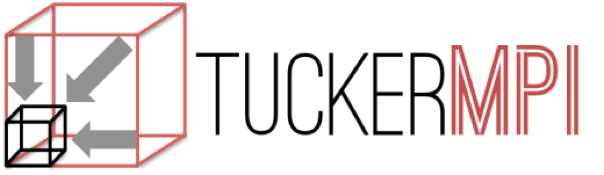
\includegraphics[scale=0.5]{tikz/chapter3/TuckerMPI-logo.png}
\end{center}

TuckerMPI uses $P$ processors organized into a $d$-dimensional $P_1\times \cdots
\times P_d$ grid such that $P = \prod_{i=1}^{d} P_i$ and that each processor
stores a $1/P$ fraction of $\mathcal{X}$. Our analysis will assume $\mathcal{X}
\in \mathbb{R}^{n\times \cdots \times n}$ and $\mathcal{G} \in
\mathbb{R}^{r\times \cdots \times r}$ to simplify cost comparison across
algorithms.

\subsection{TuckerMPI's STHOSVD} \label{sec:TuckerMPI's STHOSVD}
    \subsubsection{STHOSVD's Computational Complexity} \label{STHOSVD's Computational Complexity}

        The cost of LLSV in line \ref{line:sthosvd_llsv} is given by
        \begin{equation*}
            \sum_{j=1}^{d} \left(\frac{r^{j-1}n^{d-j+2}}{P} + \mathcal{O}(n^3)\right) \approx \frac{n^{d+1}}{P} + \mathcal{O}(dn^3),
        \end{equation*}
        where the first term is the cost of computing the $n \times n$ Gram matrix and
        the second term is the cost of sequentially computing the EVDs to leading order.
        %We perform the Eigendecomposition sequentially on a single processor and communicate $\Mx{U}_j$.
        After $\mathbf{U}_{k}$ is computed, $\mathcal{Y}$ is truncated by
        performing the TTM in line \ref{line:sthosvd_ttm}, which costs
        \begin{equation*}
            2\sum_{j=1}^{d} \frac{r^j n^{d-j+1}}{P} \approx 2\frac{rn^d}{P}.
        \end{equation*}
        Computing the Gram matrix is a factor of $\nicefrac{n}{2r}$ more expensive than
        the TTM and is the dominant cost for $n \gg r$. Sequentially truncating $\mathcal{Y}$
        leads to decreasing dimensions, so the algorithm is typically dominated by the
        first Gram matrix computation. Note that the EVD is not parallelized, which can
        be a barrier to parallel scaling when a single tensor dimension is large. We
        summarize the leading order STHOSVD flops cost in \cref{tab:flops} (shown in
        red).

    \subsubsection{STHOSVD's Communication Complexity} \label{sec:STHOSVD's Communication Complexity}

        TuckerMPI's parallel algorithm for LLSV explicitly forms the Gram
        matrix, $\mathbf{G} = \mathbf{Y}_{(k)}\mathbf{Y}_{(k)}^\intercal$,
        where $\mathbf{Y}_{(k)}$ is redistributed (if necessary) to a 1D column
        layout across $P$ processors, and then sequentially computes the EVD of
        $\mathbf{G}$. After redistribution of $\mathbf{G}$, each processor
        computes a local Gram matrix which can be sum-reduced (or all-reduced)
        prior to the EVD. At iteration $k$, the number of entries in
        $\mathcal{Y}$ is $r^{j-1}n^{d-j+1}$. The Gram matrix that is computed in
        each mode is of size $n \times n$, so the total communication cost is
        $dn^2$ for the all-reduce. Thus, the communication cost is given by
        \begin{equation*}
            \sum_{j=1}^{d} \bigg(\frac{r^{j-1}n^{d-j+1}}{P}\cdot \frac{P_j - 1}{P_j} + \mathcal{O}(n^2)\bigg) \approx \frac{n^{d}}{P}\cdot \frac{P_1 - 1}{P_1} + dn^2,
        \end{equation*}
        where we assume the redistribution cost is dominated by the first mode. However,
        note that there is no redistribution cost in mode $j$ if $P_j=1$. Finally, the
        parallel TTM also requires communication to perform a sum-reduce of local TTM
        results. Since the output of the TTM is largest in the first mode (of size
        $rn^{d-1}/P$), the communication cost of TTMs to leading order cost is
        \begin{equation*}
            \sum_{j=1}^{d} \frac{r^{j}n^{d-j}}{P}(P_j - 1) \approx \frac{rn^{d-1}}{P}(P_1 - 1).
        \end{equation*}
        Again, note there is no communication cost in mode $j$ if $P_j=1$.
        Because the largest data communicated occurs in mode 1, processor grids
        with $P_1=1$ are typically the fastest for STHOSVD (as we observe in our
        experiments). We summarize the STHOSVD communication costs in
        \cref{tab:comm} (shown in red).

\subsection{TuckerMPI's HOOI} \label{sec:TuckerMPI's HOOI}
    \subsubsection{HOOI's Computational Complexity} \label{sec:HOOI's Computational Complexity}

        Since HOOI is an iterative algorithm for Tucker decomposition, we analyze the
        cost of one HOOI iteration. Each HOOI iteration requires $d$ multi-TTMs, in all
        modes but mode-$j$, and $d$ LLSV computations to update factors matrices, in all
        modes. Once the factor matrices have been updated, the core tensor $\mathcal{G}$ is
        obtained by performing a TTM with the last factor matrix $\mathbf{U}{d}$. The cost
        of computing $d$ multi-TTMs is given by

        \begin{equation*}
            2d \sum_{i=1}^{d} \frac{r^i n^{d-i+1}}{P} \approx 2d\frac{rn^d}{P}.
        \end{equation*}

        The cost of each TTM decreases, so the first term in the summation (i.e. the
        first TTM) dominates. Multiplying the cost of the first TTM by $d$ yields the
        cost of $d$ multi-TTMs (i.e. one HOOI iteration). The cost of computing LLSV is
        given by
        \begin{equation*}
            d\frac{r^{d-1}n^2}{P} + \mathcal{O}(dn^3),
        \end{equation*}
        where the first term is the cost of computing the Gram matrix
        $\mathbf{Y}_{(k)}\mathbf{Y}_{(k)}'$ and the second term is the cost of
        computing the EVD. Finally, the core tensor at the end of each HOOI
        iteration is obtained by performing a TTM in mode-$d$ with the
        intermediate tensor $\mathcal{Y}$ and $\mathbf{U}_{d}$, which has a cost of
        $2\nicefrac{nr^{d}}{P}$ and is a lower order term. We summarize the
        leading order cost per HOOI iteration as implemented by TuckerMPI in
        \cref{tab:flops} (shown in red).


    \subsubsection{HOOI's Communication Complexity} \label{sec:HOOI's Communication Complexity}
        The communication cost of each iteration of HOOI is dominated by multi-TTMs and
        LLSV computations. Each TTM in the multi-TTM requires communication to perform a
        sum reduction to form $\mathcal{Y}$. Communication is required along the processor
        dimension corresponding to the mode in which a TTM is performed.
        %We consider two collectives for the sum reduction: a single reduce-scatter or $P_i$ reduces each with a different root.
        %If sufficient temporary storage is available, then a reduce-scatter is preferred as it is a factor of $2$ cheaper in bandwidth than performing $P_i$ reduces.
        %We assume that sufficient temporary storage is available and that the reduce-scatter is used.
        The size of $\mathcal{Y}$ decreases with each TTM, so the communication cost of a
        multi-TTM is dominated by the first TTM. Each HOOI iteration performs $d$
        multi-TTMs, where one iteration updates the factor matrix in the first mode.
        %We assume that the multi-TTM corresponding to $j=1$ in \Cref{alg:hooi} is performed in reverse order (starting with the mode-$d$ TTM) so that the largest TTM can be performed using a single GEMM call.
        The cost of communication for the multi-TTMs is given by
        \begin{multline*}
            \sum_{j=1}^d \bigg(\sum_{i=1}^{j-1} \frac{r^in^{d-i+2}}{P}(P_i-1) + \sum_{i=j+1}^{d} \frac{r^{i-1}n^{d-1+1}}{P}(P_i-1)\bigg) \\ \approx (d-1)\frac{rn^{d-1}}{P}(P_1 - 1) + \frac{rn^{d-1}}{P}(P_2 - 1).
        \end{multline*}
        The first term corresponds to the $d-1$ TTMs performed in the 1st mode and the
        second term corresponds to TTMs performed in the 2nd mode (for the multi-TTM in
        all but the 1st mode).
        %Each mode-$1$ TTM computes a local tensor of size $\frac{rn^{d-1}}{\Pi_{i = 2}^d P_i}$ which is reduce-scattered between processors in the $P_1$ dimension which yields a bandwidth cost of $\frac{rn^{d-1}}{P} (P_1 - 1)$ per TTM in the first mode.
        %When updating the first mode factor matrix, we perform the mode-$d$ TTM first.
        %The mode-$d$ TTM stores a local tensor of size $\frac{rn^{d-1}}{\Pi_{i = 1}^{d-1} P_i}$ which is communicated in the $P_d$ dimension.
        %Multiplying the cost of reduce-scatter in the mode-$1$ TTMs by $d-1$ and adding the cost of the mode-$d$ TTM (when $j = 1$) yields the total communication cost of multi-TTMs to leading order.

        Communication is also required when computing the LLSV in each mode.
        Using the same LLSV algorithm as in STHOSVD, the Gram matrix is computed
        in parallel followed by a sequential EVD. Computing the Gram matrix
        requires an all-to-all to redistribute $\mathbf{Y}_{(k)}$ so that it is
        stored in 1D-column layout. After redistribution
        $\mathbf{Y}_{k}\mathbf{Y}_{k}^\intercal$ is computed in parallel by
        performing local matrix-matrix multiplications that are sum-reduced to
        obtain the Gram matrix. The cost of communication for the LLSV is given
        by
        \begin{equation*}
            \frac{r^{d-1}n}{P} \sum_{i = 1}^{d}\left(\frac{P_i-1}{P_i}\right) + dn^2,
        \end{equation*}
        where the first term is the cost of all-to-all communication and the second term
        is the cost of sum reduction of the Gram matrix for one HOOI iteration (i.e. $d$
        calls to LLSV).
        %Each all-to-all requires redistribution of $\frac{nr^{d-1}}{P}$ local data which must be sent to $P_i$ processors, where $i$ is the mode in which LLSV is being computed.
        %This requires sending $P_i - 1$ messages each of size $\frac{1}{P_i} \cdot \frac{nr^{d-1}}{P}$.
        %Summing this cost over all $d$ modes yields the first term.
        %The second term is the cost of sum-reducing the $n$-dimensional Gram matrix, which has a message size cost of $n^2$ per mode.
        %Multiplying this cost by $d$ gives the second term.
        We summarize the HOOI communication costs as implemented by TuckerMPI in \Cref{tab:comm} (shown in red).


\subsection{TuckerMPI's Dimension Tree} \label{sec:TuckerMPI's Dimension Tree}
    \subsubsection{Dimension Tree Computational Complexity} \label{sec:Dimension Tree Computational Complexity}

        The flops cost of performing multi-TTMs using dimension trees is given by
        \begin{equation*}
            4 \sum_{i=1}^{d/2} \frac{r^i n^{d-i+1}}{P} + \mathcal{O} \left(d \sum_{i = d/2 + 1}^{d} r^i n^{d - i + 1}\right) \approx 4\frac{rn^d}{P},
        \end{equation*}
        where the first term is the cost of computing the TTMs in the first two branches
        (left and right of the root) in the dimension tree and the second term is the
        cost of computing the TTMs in all remaining branches. The largest TTMs in the
        first two branches dominate, so the cost of multi-TTMs is $4\cdot \nicefrac{rn^d}{P}$
        (i.e. the first TTM in each branch), which is a factor of $\nicefrac d2$ improvement over
        computing multi-TTMs directly. This cost is summarized in \Cref{tab:flops}.
    
    \subsubsection{Dimension Tree Communication Complexity} \label{sec:Dimension Tree Communication Complexity}

        Since the first TTM in each of the two multi-TTMs off the root dominate,
        the communication cost of multi-TTMs is given by
        \begin{equation*}
            \sum_{i=1}^{d/2}  \frac{r^in^{d-i-1}}{P}\left(P_i - 1 + P_{d-i+1} - 1\right) \approx   \frac{rn^{d-1}}{P} \left(P_1 + P_d - 2\right).
        \end{equation*}
        
        When traversing the right branch in the dimension tree shown in
        \cref{fig:dimtree}, TTMs are performed in the first $\nicefrac d2$ modes
        starting with mode $1$. The communication cost associated with TTMs in
        the right branch is the cost of a reduce-scatter on local data of size
        $\nicefrac{rn^{d-1}}{P}\cdot(P_1-1)$, which yields the first term. The
        second term is due to the communication cost associated with traversing
        the left branch in \cref{fig:dimtree}. TTMs in the left branch are
        performed in the last $\nicefrac d2$ modes starting with mode $d$. We
        perform left branch TTMs in reverse order because the mode $d$ TTM
        achieves higher local TTM performance due to the layout of the local
        tensor in memory. The communication cost associated with TTMs in the
        left branch is the same as the first term, except that the
        reduce-scatter is performed in the $P_d$ processor grid dimension.
        Therefore, processor grids with $P_1 = P_d = 1$ are typically the
        fastest for HOOI algorithms employing the dimension tree optimization
        (as we observe in our experiments).

        As shown in \cref{tab:flops,tab:comm}, introducing dimension trees
        memoization reduces the flops cost of TTMs in HOOI by a factor of $d/2$
        and the communication cost by a factor of $d-1$ in the first term.


\subsection{TuckerMPI's Subspace Iterations} \label{TuckerMPI's Subspace Iterations}
    \subsubsection{Subspace Iteration Computational Complexity.}
        Each subspace iteration requires two matrix-matrix multiplications and
        one QR decomposition. The first matrix-multiplication corresponds to the
        TTM $\mathcal{G}=\mathcal{Y} \times_k \mathbf{U}_{(k)}^\intercal$ (in the
        notation of \cref{alg:Classic-HOOI}) and the second computes the tensor
        contraction $\mathbf{Y}_{(k)}\mathbf{G}_{(k)}^\intercal$. The total computational cost of
        performing the TTM and contraction in each HOOI iteration is
        $4d\cdot\nicefrac{nr^d}{P}$. The cost of the QR decomposition of the
        matrix $\mathbf{Z} \in \mathbb{R}^{n\times r}$ in each HOOI iteration is
        $\mathcal{O}(dnr^2)$, where we assume a sequential QR decomposition. The
        total cost of performing subspace iteration in each mode across an
        entire HOOI iteration is given by
        \begin{equation*}
            4d\frac{nr^d}{P} + \mathcal{O}(dnr^2).
        \end{equation*}

        As shown in \cref{tab:flops}, the cost of LLSV using subspace iteration is a
        factor of $\nicefrac{1}{4} \cdot \nicefrac{n}{r}$ cheaper than the cost of LLSV via the
        Gram matrix.
        %When compared to the Gram computation in STHOSVD, HOOI with subspace iteration is a factor of approximately $\frac{1}{4dt} \cdot \prn+{\frac{n}{r}}$ faster.
        When comparing the sequential EVD to the sequential QR decomposition,
        the cost of the latter is a factor of
        $\mathcal{O}\left(\big(\nicefrac{n}{r}\big)^2\right)$ faster.
        %The best variant of HOOI based on the algorithmic improvements we have
        %introduced is HOOI with dimension trees and subspace iteration optimizations,
        %which we will refer to as HOSI-DT. \Cref{tab:flops} summarizes the flops cost
        %of $t$ iterations of HOSI-DT.

    \subsubsection{Subspace Iteration Communication Complexity.}
        Subspace iteration requires communication in the TTM, tensor contraction, and QR
        decomposition in each mode. The communication cost of the TTM is given by
        $\nicefrac{r^d}{P}\cdot (P_k - 1)$, where $P_k$ corresponds to the number of
        processors in the $k^\text{th}$ mode. The tensor contraction requires redistribution of
        both tensors via all-to-all communication steps. However, the all-to-all cost is
        a lower order term since it is a factor of $P_k$ cheaper than the communication
        cost associated with the TTM. Once the contraction is performed, a sum reduction
        followed by a broadcast is required to ensure that all processors can
        independently compute local QR decompositions. The communication cost of the QR
        decomposition is given by $2nr$ since $\mathbf{Z} \in \mathbf{R}^{n\times r}$ and must be
        communicated twice. As shown in \cref{tab:comm}, the total communication cost of
        the LLSV calls within an iteration of HOOI using subspace iteration is given by
        \begin{equation*}
            \frac{r^d}{P}\sum_{j=1}^{d}\left(P_j - 1\right) + 2dnr.
        \end{equation*}







\subsection{TuckerMPI's Adaptive Rank} \label{TuckerMPI's Adaptive Rank}
    \subsubsection{Core Analysis Computational Complexity} \label{sec:Core Analysis Computational Complexity}

        The cost of one RA-HOOI iteration is the same as one iteration of HOOI given in
        \cref{tab:flops}, but with the possible additional cost of performing analysis
        on the core tensor $\mathcal{G}$ to adapt the ranks for the next iteration. We solve
        the optimization problem given in \cref{eq:rankcond} exhaustively by computing
        the norm and corresponding size of every leading subtensor. This can be done
        using only $\mathcal O(dr^d)$ operations by employing a multidimensional prefix
        sum computation across the squares of the core entries. Because computational
        cost tends to be dominated by the rest of the HOOI iteration, we perform the
        core analysis sequentially, though the prefix sums are readily parallelizable.

        Assuming that this analysis is performed sequentially, the cost of the
        core analysis is $\mathcal{O}(r^d)$. The cost of the core analysis is
        dominated by the cost of computing a cumulative sum of entries in
        $\mathcal{G}$ and finding the smallest entry which meets the relative error
        tolerance. Performing these operations requires $\mathcal{O}(r^d)$
        flops. Since we need $\nicefrac nr$ to be large for HOOI to improve performance
        over STHOSVD, the cost of sequential core analysis can be performed in
        parallel, but we expect that the cost of communication would outweigh
        the benefits of parallelizing this operation.

    \subsubsection{Core Analysis Communication Complexity} \label{sec:Core Analysis Communication Complexity}

        At the end of a HOOI iteration, $\mathcal{G}$ is distributed across all processors,
        so it must be gathered on a single processor in order to perform analysis. Since
        the entire core tensor must be communicated, the all-gather cost is $r^d$ per
        HOOI iteration.
        % We opt for sequential analysis as the computation and communication costs of core analysis are low order terms when compared to the costs of TTM and LLSV.
        We demonstrate in \cref{sec:results} that the sequential cost of core analysis is typically negligible.


\begin{table*}
    \scalebox{0.862}[0.862]{
        \begin{tabular}{c|c|c|c|c|c}
            \bf Algorithm & \multicolumn{2}{|c|}{\bf LLSV} & \multicolumn{2}{|c|}{\bf TTM} & \bf Core Analysis\\ \hline\hline
            \multirow{2}{*}{\bf HOOI iteration} & \bf Gram + Eig & \textcolor{red}{$d\frac{n^2r^{d-1}}{P} + \mathcal{O}(dn^3)$} & \bf Direct & \textcolor{red}{$2d\frac{rn^d}{P}$} & \multirow{2}{*}{$\mathcal{O}(dr^d)$}\\\cline{2-5}
            & \bf Sub. Iter. & $4d\frac{nr^d}{P} + \mathcal{O}(dnr^2)$ & \bf Dim. Tree & $4\frac{rn^d}{P}$\\\hline\hline
            \bf STHOSVD & \multicolumn{2}{|c|}{\textcolor{red}{$\frac{n^{d+1}}{P} + \mathcal{O}(dn^3)$}} & \multicolumn{2}{|c|}{\textcolor{red}{$2\frac{rn^d}{P}$}} & -\\\hline
            \bf RA-HOSI-DT & \multicolumn{2}{|c|}{$\ell\left(4d\frac{nr^d}{P} + \mathcal{O}(dnr^2)\right)$} & \multicolumn{2}{|c|}{$\ell\left(4\frac{rn^d}{P}\right)$} & $\ell \left(\mathcal{O}(dr^d)\right)$\\\hline
        \end{tabular}
    }
    \caption{Leading order flops costs of LLSV (Gram + Eig and Subspace Iteration), multi-TTM (Direct and Dimension Trees) and Core Analysis algorithmic choices for HOOI and a comparison between STHOSVD and HOOI with Subspace Iteration and Dimension Trees (HOSI-DT) optimizations. We assume $\ell$ iterations of HOSI-DT are performed.}
    \label{tab:flops}
\end{table*}

\begin{table*}
    \scalebox{0.62125}[0.8]{
        \begin{tabular}{c|c|c|c|c|c}
            \bf Algorithm & \multicolumn{2}{|c|}{\bf LLSV} & \multicolumn{2}{|c|}{\bf TTM} & \bf Core Analysis\\ \hline \hline
            \multirow{2}{*}{\bf HOOI iteration} & \bf Gram + Eig & \textcolor{red}{$\frac{nr^{d-1}}{P}\sum_{i=1}^{d}\frac{P_i-1}{P_i} + dn^2$} & \bf Direct & \textcolor{red}{$(d-1)\frac{rn^{d-1}}{P}(P_1 - 1) + \frac{rn^{d-1}}{P}(P_2 - 1)$} & \multirow{2}{*}{$r^d$}\\\cline{2-5}
            & \bf Sub. Iter. & $\frac{r^d}{P}\sum_{i=1}^{d} \left(P_i - 1\right) + 2dnr$ & \bf Dim. Tree. & $\frac{rn^{d-1}}{P}(P_1 - 1) + \frac{rn^{d-1}}{P}(P_d - 1)$\\\hline\hline
            \bf STHOSVD & \multicolumn{2}{|c|}{\textcolor{red}{$\frac{n^d}{P}\frac{P_1-1}{P_1} + dn^2$}} & \multicolumn{2}{|c|}{\textcolor{red}{$\frac{rn^{d-1}}{P}(P_1 - 1)$}} & -\\\hline
            \bf RA-HOSI-DT & \multicolumn{2}{|c|}{$t\Big(\frac{r^d}{P}\sum_{i=1}^{d} (P_i - 1) + 2dnr\Big)$} & \multicolumn{2}{|c|}{$t\Big(\frac{rn^{d-1}}{P}(P_1+P_d-2)\Big)$} & $\ell \left(r^d\right)$\\\hline
        \end{tabular}
    }
    \caption{Leading order bandwidth costs of LLSV (Gram + Eig and Subspace Iteration), multi-TTM (Direct and Dimension Trees) and Core Analysis algorithmic choices for HOOI. For reference, we include a comparison between STHOSVD and HOOI with Subspace Iteration and Dimension Trees (HOSI-DT). We assume a processor grid of $P = (P_1\times \cdots \times P_d)$ and that $\ell$ iterations of HOSI-DT are performed.}
    % \AD{consider removing factors of $1 - 1/P_i$ for STHOSVD and HOOI to simplify the table, since these are easy to upper bound. Sub. iter. is a diverging series, so harder to simplify.}
    \label{tab:comm}
    % \AD{I think HOOI Gram+Eig and Sub. Iter. costs need a factor of $\sum_{i = 1}^{d} \frac{P_i - 1}{P_i}$ in the Gram bandwidth term.}
    % \AD{HOOI TTM cost implies that the mode-$1$ factor matrix is resized to the new rank. However, if $r$ increases then we do not increase size of $\Mx{U}{1}$. The asymptotic cost stays the same, but doesn't accurately capture our implementation. Also, if we assume that modes are processed in natural order then I think the next largest TTM cost should be $P_2$ and not $P_d$?}
\end{table*}

\section{Results}
    %!TEX root = ../../main.tex

\newcommand{\datapath}{}
\newcommand{\errone}{}
\newcommand{\errtwo}{}
\newcommand{\errthree}{}
\newcommand{\error}{}
\newcommand{\test}{}
\newcommand{\thresh}{}

This section presents a comparison of the
running time (strong scaling and running time breakdown) and compression (error
vs. time and error vs. compression ratio) performance of the various Tucker
algorithms presented in this work. All algorithms were implemented using the
TuckerMPI (C++/OpenMPI) library \cite{BKK20}.

\paragraph{Computing platform.} Our experiments were conducted on
NERSC Perlmutter (CPU partition). The system consists of 3072 compute nodes with
dual-socket AMD EPYC 7763 64-core CPUs. Each socket has 4 Non-Uniform Memory
Access (NUMA) regions for a total of 8 NUMA regions per node. Each NUMA region
has 64 GB of DRAM memory, therefore each CPU socket has 256 GB of DRAM for, a
total of 512 GB of memory per node.
% Each NUMA region can communicate with all the cores in its node, but it
% communicates the fastest with the 16 cores in its socket.

\paragraph{Experiments.} We perform experiments on synthetic tensors that are
randomly generated and tensors obtained from real applications. We use 3-way and
4-way tensors for the synthetic experiments, and three real datasets: Miranda
\cite{KD+20} (3-way), HCCI \cite{BCL14} (4-way), and SP \cite{KZCS16} (5-way).
The real datasets are described in more detail in \cref{sec:high_nr,sec:low_nr}.
Experiments performed on synthetic tensors are performed in single precision,
while experiments on real datasets are performed in single or double precision
depending on their storage precision on disk. Strong scaling experiments are
performed on the synthetic tensors. We show running time breakdown of both real
and synthetic experiments. For synthetic tensors we show the running time
breakdown at small and large scale to highlight how each step in a given
algorithm scales. For real tensors we vary the error tolerance and starting
ranks to show how performance breakdowns vary. Compression performance
experiments are performed only on the real datasets.
% two sets of experiments: strong scaling on
% synthetic tensors using single precision, and a comparative performance against
% the state-of-the art using the three data sets.

Even for a fixed number of processors $P$, the $d$-way processor grid has a
significant effect on all algorithms. As described in \cref{sec:TuckerMPI's STHOSVD},
STHOSVD benefits from processor grids with $P_1=1$, and HOOI variants using
dimension trees are theoretically more efficient when $P_1=P_d=1$. In addition,
for modes with small tensor dimension, a large processor dimension in that mode
may cause load imbalance due to uneven division. In all experiments, we test all
algorithms on a variety of grids, including those we expect to benefit
individual algorithms, and we report the fastest observed running times.
%For the most part,
%HOOI and HOSI prefer grids that have 1 in the last mode, HOOI-DT and HOSI-DT
%prefer algorithms that have 1 in both the first and last mode, and STHOSVD
%prefers grids that have 1 in the first mode. 
%The occasions where such pattern
%not result in their best performance for a certain experiment is when a
%processor grid mode greatly exceeds the input tensor or core tensor size for
%that mode since that creates work imbalance. 
%For example, in
%\cref{sec:synthetic_strong_scaling} for both the 3-way and 4-way experiments,
%HOSI-DT's best times came from grids that had a 1 in the first and last mode up
%to 512 cores, afterwards, it preferred grids that more evenly split the
%workload. From 1024 to 4096 cores HOSI-DT prefers grids with a 2 in the first
%and last mode. At 8192, HOSI-DT also preferred the grid that had a 2 in the
%first and last modes, but for the 3-way, it preferred grids that more evenly
%split the work. 

\subsection{Strong Scaling on Synthetic Tensors} \label{sec:synthetic_strong_scaling} 

    First, we present strong scaling
    experiments on the 3-way and 4-way synthetic tensors to demonstrate the parallel
    scaling of HOOI, HOOI-DT, HOSI, HOSI-DT, and STHOSVD. We choose tensor
    dimensions to maximize the size of the tensor that can fit on a single node (in
    single precision).
    % We present an experiment on synthetic tensors that demonstrates the parallel
    % scaling capabilities of each algorithm. Specifically, we wish to demonstrate
    % scaling of HOOI, HOOI-DT, HOSI, HOSI-DT, and STHOSVD on two synthetic
    % tensors, a 3-way and a 4-way tensor. The dimensions of each tensor were
    % chosen so that maximize the size of the tensor on single precision such that
    % the input tensor and its tucker decomposition could all fit on a single
    % node. The HOOI algorithms are run on two iterations. Since STHOSVD is not
    % an iterative algorithm, we informally refer to its runtime as a `single
    % iteration'.

    For synthetic input, we generate tensors by forming a Tucker-format tensor of specified rank and adding a specified level of noise.
    Thus, these experiments are performed for the rank-specified formulation of the Tucker approximation problem to recover the input. 
    We run for two iterations for each variant of HOOI even though we often have a sufficiently accurate approximation after a single iteration.
    We include overhead due to core analysis for the error-specified formulation in the experiments on the real datasets.
    % the rank-specified variations of all five algorithms, the input ranks are the
    % same as the ranks used to generate the tensor. In other words, we are still
    % not testing core analysis on the HOOI algorithms, and we are using the
    % rank-specified version of STHOSVD.
    The largest 3-way tensor that fits into single-node memory is a
    tensor of size $3750 \times 3750 \times 3750$. 
    We generate this tensor to
    have a rank of $30$ in all modes.
    % by multiplying factor matrices $\Mx{A}{i} \in \Rmsiz{3750, 30}$ into the core
    % tensor $\Tn{G}\in \Rmsiz{30, 30, 30}$.
    %Here, $\frac{n}{r} = 125$, and the compression ratio is $1,953,125$. 
    Similarly, we construct the 4-way tensor of size $560 \times 560 \times 560\times 
    560$ with Tucker ranks $(10,10,10,10)$.

    \begin{figure}
        \centering
        \renewcommand{\datapath}{../../data}

\begin{tikzpicture}
    \begin{axis}[
        width =0.65\textwidth,
        height=0.65\textwidth,
        xlabel={Number of Cores},
        ylabel={Time},
        ylabel near ticks,
        xlabel near ticks,
        ymode=log,
        log basis y={2},
        xmode=log,
        log basis x={2},
        xtick={1,2,4,8,16,32,64,128,256,512,1024,2048,4096,8192},
        xticklabels={1,2,4,8,16,32,64,128,256,512,1024,2048,4096,8192},
        ytick={2^(-1),1,2,4,8,16,32,64,128,256,512,1024,2048},
        x tick label style={rotate=45, anchor=east, font=\small},
        grid=both,
        legend pos=outer north east,
        % legend style={draw=none, cells={anchor=west}, font=\small},
        title={3 way},
    ]

        \addplot[color=red,mark=square,mark size=1.5pt]
        	table[x=nprocs, y=HOOI_totals, col sep=comma] {data/Cores_3way_3750_30_Single/Total_Times.csv};
         \addlegendentry{HOOI}
    
        \addplot[color=blue,mark=square,mark size=1.5pt]
        	table[x=nprocs, y=HOOI_DT_totals, col sep=comma] {/Users/joaodeoliveria/Documents/Thesis/MasterThesisDocument/data/Cores_3way_3750_30_Single/Total_Times.csv};
         \addlegendentry{HOOI-DT}
    
        \addplot[color=orange,mark=triangle,mark size=1.5pt]
        	table[x=nprocs, y=HOSI_totals, col sep=comma] {/Users/joaodeoliveria/Documents/Thesis/MasterThesisDocument/data/Cores_3way_3750_30_Single/Total_Times.csv};
         \addlegendentry{HOSI}
    
        \addplot[color=purple,mark=triangle,mark size=1.5pt]
        	table[x=nprocs, y=HOSI_DT_totals, col sep=comma] {/Users/joaodeoliveria/Documents/Thesis/MasterThesisDocument/data/Cores_3way_3750_30_Single/Total_Times.csv};
         \addlegendentry{HOSI-DT}
    
        \addplot[color=green,mark=o,mark size=1.5pt]
        	table[x=nprocs, y=STHOSVD_totals, col sep=comma] {/Users/joaodeoliveria/Documents/Thesis/MasterThesisDocument/data/Cores_3way_3750_30_Single/Total_Times.csv};
         \addlegendentry{STHOSVD}

    \end{axis}
\end{tikzpicture}
        \caption[3-way Strong Scaling]{Strong scaling comparison of Tucker
        algorithms in single precision using a 3-way $\mathbf{3750 \times 3750
        \times 3750}$ input tensor }
        \label{fig:3way_scaling}
    \end{figure}

    \begin{figure}
        \centering
        \renewcommand{\datapath}{../../data}

\begin{tikzpicture}
    \begin{axis}[
        width =0.65\textwidth,
        height=0.65\textwidth,
        xlabel={Number of Cores},
        ylabel={Time},
        ylabel near ticks,
        xlabel near ticks,
        ymode=log,
        log basis y={2},
        xmode=log,
        log basis x={2},
        xtick={1,2,4,8,16,32,64,128,256,512,1024,2048,4096,8192},
        xticklabels={1,2,4,8,16,32,64,128,256,512,1024,2048,4096,8192},
        ytick={2^(-1),1,2,4,8,16,32,64,128,256,512,1024,2048},
        x tick label style={rotate=45, anchor=east, font=\small},
        grid=both,
        legend pos=outer north east,
        % legend style={draw=none, cells={anchor=west}, font=\small},
        title={4 way},
    ]

        \addplot[color=red,mark=square,mark size=1.5pt]
        	table[x=nprocs, y=HOOI_totals, col sep=comma] {data/Cores_4way_560_10_Single/Total_Times.csv};
         \addlegendentry{HOOI}
    
        \addplot[color=blue,mark=square,mark size=1.5pt]
        	table[x=nprocs, y=HOOI_DT_totals, col sep=comma] {data/Cores_4way_560_10_Single/Total_Times.csv};
         \addlegendentry{HOOI-DT}
    
        \addplot[color=orange,mark=triangle,mark size=1.5pt]
        	table[x=nprocs, y=HOSI_totals, col sep=comma] {data/Cores_4way_560_10_Single/Total_Times.csv};
         \addlegendentry{HOSI}
    
        \addplot[color=purple,mark=triangle,mark size=1.5pt]
        	table[x=nprocs, y=HOSI_DT_totals, col sep=comma] {data/Cores_4way_560_10_Single/Total_Times.csv};
         \addlegendentry{HOSI-DT}
    
        \addplot[color=green,mark=o,mark size=1.5pt]
        	table[x=nprocs, y=STHOSVD_totals, col sep=comma] {data/Cores_4way_560_10_Single/Total_Times.csv};
         \addlegendentry{STHOSVD}

    \end{axis}
\end{tikzpicture}
        \caption[4-way Strong Scaling]{Strong scaling comparison of Tucker algorithms in single
        precision using a 4-way $\mathbf{560 \times 560 \times 560 \times 560}$
        input tensor}
        \label{fig:4way_scaling}
    \end{figure}

    Figures \ref{fig:3way_scaling} and \ref{fig:4way_scaling} shows the strong
    scaling results of the HOOI variants and STHOSVD on up to $4096$ cores for
    the 3-way and 4-way synthetic datasets. We observe that STHOSVD scales well
    to $64$ cores, attaining a speedup of $15.2\times$ over the single core
    STHOSVD run. STHOSVD continues to scale up to $2048$ cores, but achieves
    only a modest speedup of $1.3\times$ over the $64$ core run. This is due to
    TuckerMPI's limitation of having a sequential EVD implementation. In
    contrast, the 4-way STHOSVD strong scaling experiment shows good scaling up
    to $8192$ cores, achieving a speedup of $937\times$ over the single core
    run. This difference in STHOSVD performance is explained by the tensor
    dimension: a sequential EVD of a matrix of dimension 560 does not become the
    bottleneck until $P$ is large. \AD{Decrease size of the images}
    %The high $\frac{n}{r}$ of the 3-way experiment makes it so that LLSV's
    %eigenvalue decomposition subroutine is the limiting factor, which is made
    %worse due to the sequential implementation. This is not the same as on the
    %4-way case as the lower $\frac{n}{r}$ makes the TTMs be the bottleneck.

    When comparing the two HOOI variants (which use Gram SVD), we observe that HOOI-DT yields a
    sequential speedup of $1.4\times$ over HOOI's direct TTM implementation for
    the 3-way tensor. For the 4-way tensor, HOOI-DT achieves a sequential
    speedup of $5.4\times$ faster than HOOI. When comparing parallel scaling in
    the 3-way case, we see that HOOI and HOOI-DT scale to $16$ cores with a
    speedup of $3.5\times$ and $2.8\times$, respectively, over their single core
    runs. However, neither variant scales beyond $16$ cores for the 3-way
    tensor because of the sequential EVD bottlenecks. 
    For the 4-way tensor, HOOI and HOOI-DT scale to $8192$ cores with a
    speedup of $629\times$ and $346\times$, respectively, over their single core
    runs.
    % However, neither HOOI variant achieves a speedup over STHOSVD at $8192$ cores.
    The performance of HOOI and HOOI-DT degrades at $128$ cores (single node)
    because both variants are memory-bandwidth bound, and we saturate bandwidth
    at $64$ cores. HOOI and HOOI-DT continue scaling beyond $128$ cores
    (multi-node scaling) because memory bandwidth increases. 
    As can be seen in the 4096 core plots of \cref{fig:scaling_breakdown},
    HOOI and HOOI-DT suffer from the problem of the sequential EVD, and they are approximately twice as
    slow as STHOSVD because they do twice as many EVDs over two iterations.


    HOSI and HOSI-DT show significantly better scaling on the 3-way tensor when
    compared to STHOSVD and the HOOI variants because of the difference in LLSV
    subroutines. HOSI-DT achieves sequential speedups of $6.5\times$ and
    $1.7\times$ over STHOSVD and HOOI-DT, respectively. The HOSI variants scale
    to 4096 cores with HOSI-DT achieving significant parallel speedups of
    $259\times$ and $515\times$ over STHOSVD and HOOI-DT, respectively. HOSI-DT
    is also the fastest Tucker variant for the 4-way experiment attaining
    speedups of $1.5\times$ and $2.9\times$ over STHOSVD and HOOI-DT,
    respectively when comparing the best running times of each algorithm. HOSI
    and HOSI-DT exhibit similar memory bandwidth scaling behavior as the HOOI
    variants where performance degrades at $128$ cores (single node) and
    continues to scale beyond $128$ cores (multi-node scaling).
    These can be seen on \Cref{fig:scaling_breakdown}. We chose to showcase the
    breakdown using 1 core and using 4096 cores.

    \begin{figure}
        \centering
        \newcommand{\itermax}{2}
\pgfmathsetmacro{\n}{\itermax - 1}
\renewcommand{\datapath}{data}

\newcommand{\ngp}[3]{
\nextgroupplot[title={#1: #3 Core(s)}]
    \foreach \i in {0, ..., \n} {
        \addplot[
            ybar,
            color=blue,
            fill=blue!25
            ] 
            table[x=Algorithms, y=TTM_Computation_Iter\i, col sep=comma] {\datapath/Cores_#1_#2/N#3_summary.csv};
        \addplot[
            ybar,
            color=blue,
            fill=blue!50
            ] 
            table[x=Algorithms, y=TTM_Communication_Iter\i, col sep=comma] {\datapath/Cores_#1_#2/N#3_summary.csv};
        \addplot[
            ybar,
            color=red,
            fill=red!25
            ] 
            table[x=Algorithms, y=GramLQ_Computation_Iter\i, col sep=comma] {\datapath/Cores_#1_#2/N#3_summary.csv};
        \addplot[
            ybar,
            color=red,
            fill=red!50
            ] 
            table[x=Algorithms, y=GramLQ_Communication_Iter\i, col sep=comma] {\datapath/Cores_#1_#2/N#3_summary.csv};
        \addplot[
            ybar,
            color=yellow,
            fill=yellow!50
            ] 
            table[x=Algorithms, y=EigSVD_Iter\i, col sep=comma] {\datapath/Cores_#1_#2/N#3_summary.csv};
    }
}

\begin{tikzpicture}
    \begin{groupplot}[
        group style={
            group size=2 by 2,
            horizontal sep=2cm,
            vertical sep=2cm,
        },
        width=0.4\textwidth,
        height=0.4\textwidth,
        ylabel near ticks,
        xlabel near ticks,
        ybar stacked,
        xtick=data,
        xticklabels={HOOI, HOOI-DT, HOSI, HOSI-DT, STHOSVD},
        symbolic x coords={HOOI, HOOI-DT, HOSI, HOSI-DT, STHOSVD},
        ylabel={Time},
        y label style = {yshift=-.1cm},
        %xlabel={Algorithms},
        ymin=0,
        grid=both,
        x tick label style={rotate=30, anchor=east, yshift=-.1cm},
        title style={yshift=-1.5ex},
    ]
    
    % First plot
    % \nextgroupplot[title=Plot 1: Hello]
    % \addplot[blue, thick] {x^2};
    \ngp{3way}{3750_30_Single}{1}
    
    % % % Second plot
    % % \nextgroupplot[title=Plot 2: World, ylabel={}]
    % % \addplot[red, thick] {sin(deg(x))};
    \ngp{3way}{3750_30_Single}{4096}

    % % % First plot
    % % \nextgroupplot[title=Plot 1: Hello]
    \ngp{4way}{560_10_Single}{1}
    
    % % % Second plot
    % % \nextgroupplot[title=Plot 2: World, ylabel={}]
    \ngp{4way}{560_10_Single}{4096}
    
    \end{groupplot}
\end{tikzpicture}
        \caption[Running Time Breakdown for Sunthetic Datasets]{Running time breakdown for the synthetic 3-way (top) and 4-way (bottom) tensors}
        \label{fig:scaling_breakdown}
    \end{figure}
    
    \paragraph{3-way.} Observing the single-node scaling (1 to 128) of the 3-way
    experiment, we notice that all HOOI algorithms outperform STHOSVD, with
    HOSI and HOSI-DT being much further ahead of the competition since the large
    $\frac{n}{r}$ ratio of this experiment implies a LLSV bottleneck and these
    two algorithms avoid that. Here, STHOSVD is much slower because it does a
    more expensive LLSVs before the TTMs whereas the HOOI algorithms reduce this
    cost by performing the TTMs beforehand. Starting from 32 nodes, STHOSVD
    begins to outperform HOOI and HOOI-DT due to the cost of the LLSV.
    \Cref{fig:scaling_breakdown} demonstrates that the cost of LLSV is the same
    for HOOI, HOOI-DT and STHOSVD, but because HOOI must perform two
    iterations, it takes twice as long. In fact, we see that the three
    algorithms stagnate at large scaling due to TuckerMPI's limitation of having
    a sequential eigenvalue computation. Though HOSI and HOSI-DT still perform
    two iterations, neither of them need to pay the cost of the sequential
    eigenvalue decomposition. Even with a sequential QR decomposition, they
    still scale best, with the lesser TTM cost of HOSI-DT making it the best out
    of these five algorithms.

    For the 3-way synthetic tensor on 1 core, it can be seen that the cost of
    the Gram computation is the bottleneck for STHOSVD. The TTM cost for the
    dimension tree algorithms are cheaper, as expected. HOSI-DT is faster than
    HOOI-DT simply because of the smaller cost for the LLSV computations. The
    two iterations for all HOOI algorithms are faster than the `single
    iteration' for STHOSVD. However, that is not the case for the 4096 cores
    experiment. Now, the TTM costs for all algorithms are negligible due to the
    parallel scaling. The Gram computation for STHOSVD is also negligible now
    for the same reasons. The bottleneck at this scale is now the Eigenvalue
    computation. The reason why HOOI, HOOI-DT, and STHOSVD stagnate over the
    high number of cores on \Cref{fig:3way_scaling} is because of TuckerMPI's
    limitation of having a sequential eigenvalue computation, and the reason why
    HOOI and HOOI-DT are twice as expensive on multi-node experiments is because
    they must do two iterations, this fact can be visualized on the breakdown
    for the 4096 cores experiment.

    \paragraph{4-way.} In this experiment, HOOI-DT and HOSI-DT are the ones that
    get a comparative headstart since the small $\frac{n}{r}$ ratio of this
    experiment implies a TTM bottleneckm and these two algorithms avoid that.
    They diverge around 128 cores for the same reasons mentioned above as
    HOOI-DT must pay the cost of two expensive eigenvalue computation. For that
    matter, STHOSVD still eventually catches up to HOOI-DT, but now this
    happens at 512 cores as opposed to 32. For this reason, HOSI eventually
    closes the gap to HOSI-DT, with STHOSVD being not too far behind simply
    because of the smaller $\frac{n}{r}$.

    \paragraph{Overall} There are two factors that are pertinent to both 3-way and 4-way
    experiments. The first is the spike noticible at 128 for most (some more
    than others) of the algorithms. These come from a choice of configuration of
    the slurm jobs regarding the binding of NUMA regions to the cores. There
    were two main options available to run these experiments with,
    \textit{cores} and \textit{map\_ldom}. The former assigns all the NUMA
    regions of the node to the running cores, and the latter we most perform a
    manual assignment of the NUMA regions which gives us more control. We are
    not utilizing the full potential of a node from 1 to 64 cores, as there are
    more cores available, but the \textit{cores} configuration still assigns all
    the NUMA regions of the node to the running cores, so these cores have more
    memory than what is `pertinent' to them. Thus, when we first use the full
    potential of a node at 128 cores, there is now a competition for resources.
    Running the \textit{map\_ldom} configuration allows us to bypass that
    limitation, so from 1 to 64 cores we only assign NUMA regions that would be
    `pertinent' to those cores assuring a steady parallel scaling in terms of
    memory. This makes the experiments from 1 to 32 nodes equally slower to all
    five algorithms. In other words it removes the spike, simply because the
    rate of increase is steady now. The other factor regards why HOSI and
    HOSI-DT stop scaling at 8192 cores, the reason is 42. 

\subsection{Performance on Simulation Datasets} \label{sec:performance_comparisons} 

    We turn our focus for the error-specified comparison of our best algorithm,
    HOSI-DT, and the state-of-the-art, STHOSVD. The data sets are decomposed
    using three error tolerances; 0.1 (``high compression''), 0.05 (``mid compression''), and 0.01 (``low compression''). 
    Furthermore, we
    showcase HOSI-DT through three different types of starting ranks for each
    error tolerance. Perfect starting ranks are the same as the final ranks of
    STHOSVD given the maximum relative error threshold. We overshoot and
    undershoot the same starting ranks by 25\% above and below to force our
    algorithm to respectively increase and decrease ranks on the first
    iteration. We cap the number of iterations for HOSI-DT at 3. Though all
    three iterations are shown in the Error vs Time and Error vs Size plots, the
    running time breakdown plots show  the breakdown only for however many
    iterations it took for HOSI-DT to reach the desired error threshold. For
    example, the top right plot of \cref{fig:HCCI_breakdown} it can be seen that
    the HOSI-DT (Over) 0.1 threshold reached the desired at the first iteration,
    so we don't show the breakdown for the second iteration despite its total
    time being shown on \cref{fig:HCCI}.

    \subsubsection{Miranda (3-way)}\label{sec:high_nr}
        The Miranda dataset is a three-dimensional simulation data of the
        density ratios of non-reacting flow of viscous fluids \cite{KD+20}. Each
        of its dimensions is 3072, and it is stored in single
        precision requiring 115 GB.
        Our experiments use 1024 cores (8 nodes) for all algorithms.

        \begin{figure}
            \centering
            \renewcommand{\datapath}{data/Miranda/N8_n1024}
            \renewcommand{\thresh}{1e-01,5e-02,1e-02}
            %!TEX root = ../../main.tex

% need to define \datapath and \thresh (set of error thresholds)

\newcommand{\algorithmname}{HOSI_DT}

\pgfplotsset{HOOIstyle/.style={
	red,
	mark=o,
	point meta = {\thisrow{STHOSVD_Size}/\thisrow{HOSI_DT_Size}},
	every node near coord/.append style={
		above right,
		inner sep=1pt,
		yshift=1ex
	}
}}
\pgfplotsset{STHOSVDstyle/.style={
	blue,
	mark=square*,
	only marks
}}


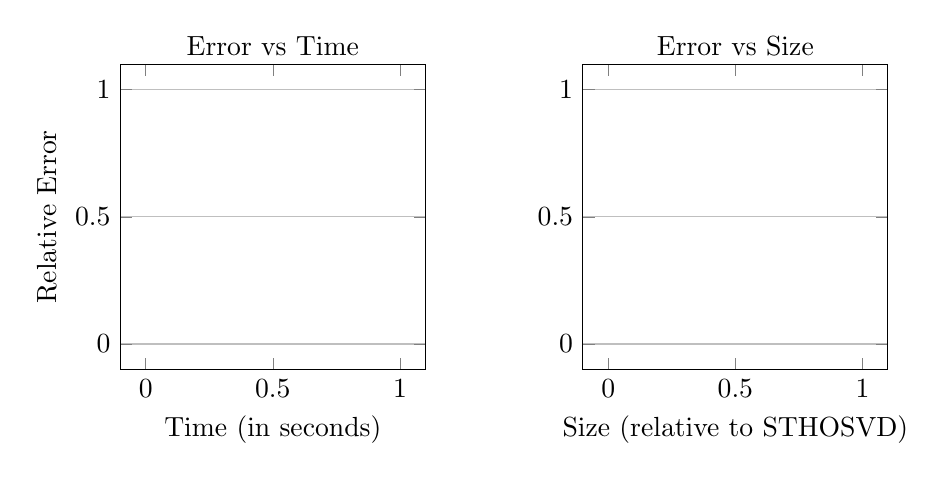
\begin{tikzpicture}
    \begin{groupplot}[
        group style={
            group size=2 by 1,
            xlabels at=edge bottom,
            ylabels at=edge left,
            horizontal sep=2cm,
            vertical sep=2cm,
        },
        width= 0.45\textwidth,
        height=0.45\textwidth,
        ylabel=Relative Error,
        ylabel near ticks,
        xlabel near ticks,
        ymajorgrids=true,
        legend to name=namedlegend,
        legend style={draw=none, cells={anchor=west}, font=\small,
        legend columns=2},
        title style={yshift=-1.5ex},
      ]
        % First plot: error vs time
        \nextgroupplot[
            title=Error vs Time, 
            xlabel=Time (in seconds),
            ytick = \thresh,
            yticklabel style={/pgf/number format/fixed}
        ]

	\foreach \t in \thresh {
		\addplot [HOOIstyle,mark=triangle] table[x=\algorithmname_Time, y=\algorithmname_Error, col sep=comma] {\datapath_\t_Over.csv};
        		\addplot [HOOIstyle,mark=star] table[x=\algorithmname_Time, y=\algorithmname_Error, col sep=comma] {\datapath_\t_Perfect.csv};
        		\addplot [HOOIstyle,mark=square] table[x=\algorithmname_Time, y=\algorithmname_Error, col sep=comma] {\datapath_\t_Under.csv};
        		\addplot [STHOSVDstyle] table[x=STHOSVD_Time, y=STHOSVD_Error, col sep=comma] {\datapath_\t_Under.csv};	
	}
      
        % Second plot: error vs relative size
        \nextgroupplot[
            title=Error vs Size,
            xlabel=Size (relative to STHOSVD),
            ytick = \thresh,
            yticklabel style={/pgf/number format/fixed}
        ]
        
        \foreach \t in \thresh {
        		\addplot[HOOIstyle,mark=triangle] table [x expr = (\thisrow{HOSI_DT_Size}/\thisrow{STHOSVD_Size}), y=HOSI_DT_Error, col sep=comma] {\datapath_\t_Over.csv};
        		\addplot[HOOIstyle,mark=star] table [x expr = (\thisrow{HOSI_DT_Size}/\thisrow{STHOSVD_Size}), y=HOSI_DT_Error, col sep=comma] {\datapath_\t_Perfect.csv};
        		\addplot[HOOIstyle,mark=square] table [x expr = (\thisrow{HOSI_DT_Size}/\thisrow{STHOSVD_Size}), y=HOSI_DT_Error, col sep=comma] {\datapath_\t_Under.csv};
        		\addplot[STHOSVDstyle] table [x expr = (\thisrow{STHOSVD_Size}/\thisrow{STHOSVD_Size}), y=STHOSVD_Error, col sep=comma] {\datapath_\t_Under.csv};
        }

        \addlegendimage{mark=triangle, color=red}
        \addlegendentry{HOSI-DT Over}
        \addlegendimage{mark=star, color=red}
        \addlegendentry{HOSI-DT Perfect}
        \addlegendimage{mark=square, color=red}
        \addlegendentry{HOSI-DT Under}
        \addlegendimage{mark=square*, color=blue, only marks}
        \addlegendentry{STHOSVD}
    \end{groupplot}
\end{tikzpicture}

% Place the legend below the figure
\begin{center}
    \ref{namedlegend}
\end{center}

 

            \caption[Miranda Dataset - Progression of Time, Trror, and Relative Size]{Progression of time, error, and relative size over 3 iterations of rank-adaptive HOSI-DT on the Miranda dataset using 1024 cores.}
            \label{fig:miranda}
        \end{figure}

        \begin{figure}
            \centering
            \renewcommand{\datapath}{data/Miranda/N8_n1024}
            \renewcommand{\thresh}{1e-01,5e-02,1e-02}
            %!TEX root = ../../main.tex


\newcommand{\maxiter}{3}
\pgfmathsetmacro{\n}{\maxiter - 1}

\begin{tikzpicture}
    \begin{axis}[
        hide axis, % Hide the dummy axis
        axis lines=none,
        xmin=0, xmax=1,
        ymin=0, ymax=1,
        width= 0.45\textwidth,
        height=0.45\textwidth,
        legend style={fill=white, at={(2.25, -0.515)}, anchor=north east, font=\small},
        legend columns=1, % Arrange legend in one column
        reverse legend
    ]   
        \addplot [color=white, fill=white, mark=square*,opacity=0] coordinates {(0,0)};
        \addlegendentry{}

        \addlegendimage{mark=square*, color=blue!25, fill=blue!25, only marks, mark options={scale=2.5, fill=blue!25}}
        \addlegendentry{TTM Comp}

        \addlegendimage{mark=square*, color=blue!50, fill=blue!50, only marks, mark options={scale=2.5, fill=blue!50}}
        \addlegendentry{TTM Comm}

        \addlegendimage{mark=square*, color=red!25, fill=red!25, only marks, mark options={scale=2.5, fill=red!25}}
        \addlegendentry{Contraction Comp}

        \addlegendimage{mark=square*, color=red!50, fill=red!50, only marks, mark options={scale=2.5, fill=red!50}}
        \addlegendentry{Contraction Comm}

        \addlegendimage{mark=square*, color=yellow!50, fill=yellow!50, only marks, mark options={scale=2.5, fill=yellow!50}}
        \addlegendentry{Eig/QR}

        \addlegendimage{mark=square*, color=green!25, fill=green!25, only marks, mark options={scale=2.5, fill=green!25}}
        \addlegendentry{Core Comp}
        
        \addlegendimage{mark=square*, color=green!50, fill=green!50, only marks, mark options={scale=2.5, fill=green!50}}
        \addlegendentry{Core Comm}
    \end{axis}

    \begin{groupplot}[
        group style={
            group size=2 by 2,
            horizontal sep=2cm,
            vertical sep=2cm,
        },
        ybar stacked,
        symbolic x coords={HOSI-DT-Under, HOSI-DT-Perfect, HOSI-DT-Over, STHOSVD},
        xticklabels={Under, Perfect, Over, STHOSVD},
        xtick=data,
        ylabel={Time},
        ylabel style = {yshift=-.675cm},
        ymajorgrids=true,
        width=0.45\textwidth,
        height=0.45\textwidth,
        x tick label style={rotate=30, anchor=east},
        title style={yshift=-1.5ex},
    ]

    \xintFor #1 in \thresh \do {
        \nextgroupplot[title = {#1 Error}]
        \foreach \i in {0, ..., \n} {    
            \addplot[ybar,color=blue,fill=blue!25] 
            		table[x=Algorithm, y=TTM_Computation_Iter_\i, col sep=comma] {\datapath_#1_Breakdown.csv};  
		
            \addplot[ybar,color=blue,fill=blue!50] 
            		table[x=Algorithm, y=TTM_Communication_Iter_\i, col sep=comma] {\datapath_#1_Breakdown.csv};
		
            \addplot[ybar,color=red,fill=red!25] 
            		table[x=Algorithm, y=GramLQ_Computation_Iter_\i, col sep=comma] {\datapath_#1_Breakdown.csv};
		
            \addplot[ybar,color=red,fill=red!50] 
    		table[x=Algorithm, y=GramLQ_Communication_Iter_\i, col sep=comma] {\datapath_#1_Breakdown.csv};
		
            \addplot[ybar,color=yellow,fill=yellow!50] 
    		table[x=Algorithm, y=EigSVD_Iter_\i, col sep=comma] {\datapath_#1_Breakdown.csv};
		
            \addplot[ybar,color=green,fill=green!25] 
    		table[x=Algorithm, y=Core_Analysis_Iter_\i, col sep=comma] {\datapath_#1_Breakdown.csv};
		
            \addplot[ybar,color=green,fill=green!50] 
    		table[x=Algorithm, y=Core_Gathering_Iter_\i, col sep=comma] {\datapath_#1_Breakdown.csv};
        }
    }

\end{groupplot}
\end{tikzpicture}

            \caption[Miranda Dataset - Running Time Breakdown]{Running time breakdown for the Miranda dataset using 1024 cores under different levels of compression.}
            \label{fig:miranda_breakdown}
        \end{figure}

        %% Just need to remove the second half of the paragraph. 
        \Cref{fig:miranda} demonstrates that for all error tolerances, three
        iterations of HOSI-DT combined is faster than STHOSVD. But as mentioned
        earlier, we focus on the least amount of iterations required to reach
        the desired error threshold. It is in high- and
        mid-compression where we find the most speedup. Precisely, perfect ranks
        achieve speedups of $82\times$ for high-compression and $25\times$ for
        mid-compression, undershooting the ranks achieves speedups of $91\times$
        for high-compression and $35\times$ for mid-compression, and
        overshooting the ranks achieves speedups of $156\times$ for
        high-compression and $47\times$ for mid-compression. Low-compression is
        the first scenario where we observe nonnegligible costs of the core
        analysis subroutine. 
        %Regardless, RA-HOSI-DT achieves speedups of
        %$1.3\times$ for perfect ranks, $1.9\times$ for undershooting ranks and
        %$1.5\times$ for overshooting ranks. 
        %These reported speedups are
        %considering all three iterations, but \cref{fig:miranda_breakdown}
        %indicates that no matter the compression, perfect and undershooting
        %ranks require only two iterations to achieve the specified error,
        %overshooting the ranks only requires one iteration. 
        %Thus, considering
        %only our fastest runs to get under the threshold (which are all rank
        %overshots) we have speedups of $156\times$ for high-compression,
        %$47\times$ for mid-compression, and $3\times$ for low compression. 
        For
        high-compression, the best relative compression ratio is $69\%$ which
        occurs at perfect ranks, mid-compression achieves a $10\%$ improvement
        using perfect ranks, and low-compression has better compression at $6\%$
        when underestimating the ranks.

    \subsubsection{HCCI (4-way) and SP (5-way)} \label{sec:low_nr}
    
        We combine the discussion of the HCCI and SP datasets results, as the results are qualitatively similar. The Homogeneous Charge Compression Ignition (HHCI)
        dataset is generated from a numerical simulation of combustion
        \cite{BCL14}. The dimension of the 4-way dataset is $672\times 672\times
        33\times 626$ stored in double precision for a total of 75 GB. Thus, we
        can fit it on a single node and use all 128 cores. The first
        two modes are spatial dimensions, the third mode corresponds to 33
        variable, and the fourth mode corresponds to time steps. 
        The SP dataset is generated from the simulation of a statistically
        stationary planar methane-air flame \cite{KZCS16}. This 5-way dataset has
        dimensions $500\times 500\times 500\times 11\times 400$ stored in double
        precision and requires 4.4 TB in storage.
        For these experiments, we use 2048 cores (16 nodes). 
        The first three modes are spatial dimensions, the fourth mode
        corresponds to 11 variables, and the last mode corresponds to time steps.

        In the case where we are dominated by the TTMs, the comparisons between
        HOSI-DT and STHOSVD are less extreme. \Cref{fig:HCCI} shows that on
        low-compression, STHOSVD is faster than any of the starting ranks of
        HOSI-DT to get to the desired threshold. However, for high- and
        mid-compression HOSI-DT achieves speedups when overshooting the ranks,
        specifically $1.9\times$ for high-compression and $1.4\times$ for
        low-compression, neither of which achieved better compression.
        \Cref{fig:HCCI_breakdown} shows the breakdown times of these speedups.
        However, HODI-DT achieves better compression with perfect and under
        ranks for all error tolerances, but always requiring three iterations to
        do so. 
        
        \Cref{fig:SP} shows that we can typically obtain better compression
        after three iterations. For example, overestimating the ranks for low
        compression yields a speedup of $1.1\times$ after 1 iteration, but we do
        not obtain better compression. Similar to HCCI, three iterations
        produces a smaller Tucker approximation but takes over twice as long.
        However, for high compression, starting from perfect and underestimates
        of the ranks achieve a $27\%$ and $8\%$ improvement on compression over
        STHOSVD after two iterations, respectively. In another example,
        \cref{fig:SP_breakdown} shows that when starting from perfect estimates
        of the ranks for mid compression, HOSI-DT gets the desired error
        tolerance and same compression ratio in less time than STHOSVD, with
        HOSI-DT achieving a $1.4\times$ speedup.
        

        \begin{figure}
            \centering
            \renewcommand{\datapath}{data/HCCI/N1_n128}
            \renewcommand{\thresh}{1e-01,5e-02,1e-02}
            %!TEX root = ../../main.tex

% need to define \datapath and \thresh (set of error thresholds)

\newcommand{\algorithmname}{HOSI_DT}

\pgfplotsset{HOOIstyle/.style={
	red,
	mark=o,
	point meta = {\thisrow{STHOSVD_Size}/\thisrow{HOSI_DT_Size}},
	every node near coord/.append style={
		above right,
		inner sep=1pt,
		yshift=1ex
	}
}}
\pgfplotsset{STHOSVDstyle/.style={
	blue,
	mark=square*,
	only marks
}}


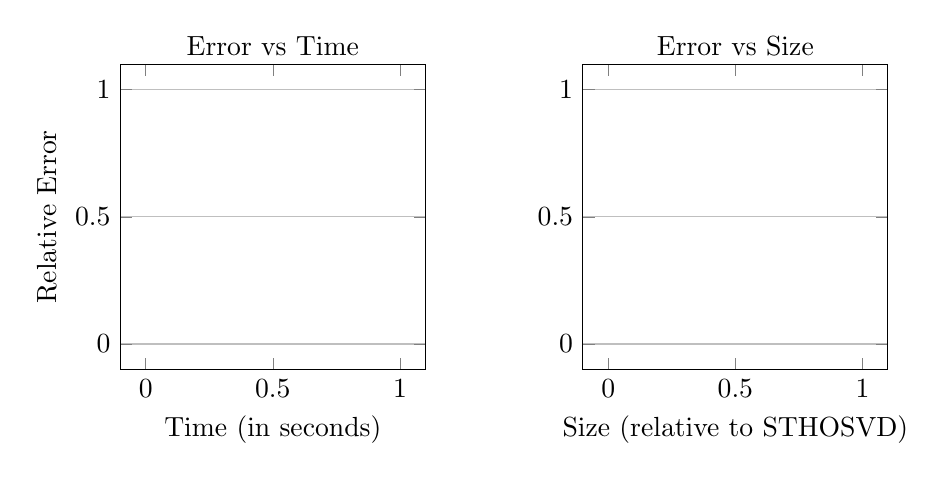
\begin{tikzpicture}
    \begin{groupplot}[
        group style={
            group size=2 by 1,
            xlabels at=edge bottom,
            ylabels at=edge left,
            horizontal sep=2cm,
            vertical sep=2cm,
        },
        width= 0.45\textwidth,
        height=0.45\textwidth,
        ylabel=Relative Error,
        ylabel near ticks,
        xlabel near ticks,
        ymajorgrids=true,
        legend to name=namedlegend,
        legend style={draw=none, cells={anchor=west}, font=\small,
        legend columns=2},
        title style={yshift=-1.5ex},
      ]
        % First plot: error vs time
        \nextgroupplot[
            title=Error vs Time, 
            xlabel=Time (in seconds),
            ytick = \thresh,
            yticklabel style={/pgf/number format/fixed}
        ]

	\foreach \t in \thresh {
		\addplot [HOOIstyle,mark=triangle] table[x=\algorithmname_Time, y=\algorithmname_Error, col sep=comma] {\datapath_\t_Over.csv};
        		\addplot [HOOIstyle,mark=star] table[x=\algorithmname_Time, y=\algorithmname_Error, col sep=comma] {\datapath_\t_Perfect.csv};
        		\addplot [HOOIstyle,mark=square] table[x=\algorithmname_Time, y=\algorithmname_Error, col sep=comma] {\datapath_\t_Under.csv};
        		\addplot [STHOSVDstyle] table[x=STHOSVD_Time, y=STHOSVD_Error, col sep=comma] {\datapath_\t_Under.csv};	
	}
      
        % Second plot: error vs relative size
        \nextgroupplot[
            title=Error vs Size,
            xlabel=Size (relative to STHOSVD),
            ytick = \thresh,
            yticklabel style={/pgf/number format/fixed}
        ]
        
        \foreach \t in \thresh {
        		\addplot[HOOIstyle,mark=triangle] table [x expr = (\thisrow{HOSI_DT_Size}/\thisrow{STHOSVD_Size}), y=HOSI_DT_Error, col sep=comma] {\datapath_\t_Over.csv};
        		\addplot[HOOIstyle,mark=star] table [x expr = (\thisrow{HOSI_DT_Size}/\thisrow{STHOSVD_Size}), y=HOSI_DT_Error, col sep=comma] {\datapath_\t_Perfect.csv};
        		\addplot[HOOIstyle,mark=square] table [x expr = (\thisrow{HOSI_DT_Size}/\thisrow{STHOSVD_Size}), y=HOSI_DT_Error, col sep=comma] {\datapath_\t_Under.csv};
        		\addplot[STHOSVDstyle] table [x expr = (\thisrow{STHOSVD_Size}/\thisrow{STHOSVD_Size}), y=STHOSVD_Error, col sep=comma] {\datapath_\t_Under.csv};
        }

        \addlegendimage{mark=triangle, color=red}
        \addlegendentry{HOSI-DT Over}
        \addlegendimage{mark=star, color=red}
        \addlegendentry{HOSI-DT Perfect}
        \addlegendimage{mark=square, color=red}
        \addlegendentry{HOSI-DT Under}
        \addlegendimage{mark=square*, color=blue, only marks}
        \addlegendentry{STHOSVD}
    \end{groupplot}
\end{tikzpicture}

% Place the legend below the figure
\begin{center}
    \ref{namedlegend}
\end{center}

 

            \caption[HCCI Dataset - Progression of Time, Error, and Relative Size]{Progression of time, error, and relative size over 3 iterations of rank-adaptive HOSI-DT on the HCCI dataset using 128 cores.}
            \label{fig:HCCI}
        \end{figure}
        \begin{figure}
            \centering
            \renewcommand{\datapath}{data/HCCI/N1_n128}
            \renewcommand{\thresh}{1e-01,5e-02,1e-02}
            %!TEX root = ../../main.tex


\newcommand{\maxiter}{3}
\pgfmathsetmacro{\n}{\maxiter - 1}

\begin{tikzpicture}
    \begin{axis}[
        hide axis, % Hide the dummy axis
        axis lines=none,
        xmin=0, xmax=1,
        ymin=0, ymax=1,
        width= 0.45\textwidth,
        height=0.45\textwidth,
        legend style={fill=white, at={(2.25, -0.515)}, anchor=north east, font=\small},
        legend columns=1, % Arrange legend in one column
        reverse legend
    ]   
        \addplot [color=white, fill=white, mark=square*,opacity=0] coordinates {(0,0)};
        \addlegendentry{}

        \addlegendimage{mark=square*, color=blue!25, fill=blue!25, only marks, mark options={scale=2.5, fill=blue!25}}
        \addlegendentry{TTM Comp}

        \addlegendimage{mark=square*, color=blue!50, fill=blue!50, only marks, mark options={scale=2.5, fill=blue!50}}
        \addlegendentry{TTM Comm}

        \addlegendimage{mark=square*, color=red!25, fill=red!25, only marks, mark options={scale=2.5, fill=red!25}}
        \addlegendentry{Contraction Comp}

        \addlegendimage{mark=square*, color=red!50, fill=red!50, only marks, mark options={scale=2.5, fill=red!50}}
        \addlegendentry{Contraction Comm}

        \addlegendimage{mark=square*, color=yellow!50, fill=yellow!50, only marks, mark options={scale=2.5, fill=yellow!50}}
        \addlegendentry{Eig/QR}

        \addlegendimage{mark=square*, color=green!25, fill=green!25, only marks, mark options={scale=2.5, fill=green!25}}
        \addlegendentry{Core Comp}
        
        \addlegendimage{mark=square*, color=green!50, fill=green!50, only marks, mark options={scale=2.5, fill=green!50}}
        \addlegendentry{Core Comm}
    \end{axis}

    \begin{groupplot}[
        group style={
            group size=2 by 2,
            horizontal sep=2cm,
            vertical sep=2cm,
        },
        ybar stacked,
        symbolic x coords={HOSI-DT-Under, HOSI-DT-Perfect, HOSI-DT-Over, STHOSVD},
        xticklabels={Under, Perfect, Over, STHOSVD},
        xtick=data,
        ylabel={Time},
        ylabel style = {yshift=-.675cm},
        ymajorgrids=true,
        width=0.45\textwidth,
        height=0.45\textwidth,
        x tick label style={rotate=30, anchor=east},
        title style={yshift=-1.5ex},
    ]

    \xintFor #1 in \thresh \do {
        \nextgroupplot[title = {#1 Error}]
        \foreach \i in {0, ..., \n} {    
            \addplot[ybar,color=blue,fill=blue!25] 
            		table[x=Algorithm, y=TTM_Computation_Iter_\i, col sep=comma] {\datapath_#1_Breakdown.csv};  
		
            \addplot[ybar,color=blue,fill=blue!50] 
            		table[x=Algorithm, y=TTM_Communication_Iter_\i, col sep=comma] {\datapath_#1_Breakdown.csv};
		
            \addplot[ybar,color=red,fill=red!25] 
            		table[x=Algorithm, y=GramLQ_Computation_Iter_\i, col sep=comma] {\datapath_#1_Breakdown.csv};
		
            \addplot[ybar,color=red,fill=red!50] 
    		table[x=Algorithm, y=GramLQ_Communication_Iter_\i, col sep=comma] {\datapath_#1_Breakdown.csv};
		
            \addplot[ybar,color=yellow,fill=yellow!50] 
    		table[x=Algorithm, y=EigSVD_Iter_\i, col sep=comma] {\datapath_#1_Breakdown.csv};
		
            \addplot[ybar,color=green,fill=green!25] 
    		table[x=Algorithm, y=Core_Analysis_Iter_\i, col sep=comma] {\datapath_#1_Breakdown.csv};
		
            \addplot[ybar,color=green,fill=green!50] 
    		table[x=Algorithm, y=Core_Gathering_Iter_\i, col sep=comma] {\datapath_#1_Breakdown.csv};
        }
    }

\end{groupplot}
\end{tikzpicture}

            \caption[HCCI - Running Time Breakdown]{Running time breakdown for the HCCI dataset using 128 cores under different levels of compression.}
            \label{fig:HCCI_breakdown}
        \end{figure}
        

        \begin{figure}
            \centering
            \renewcommand{\datapath}{data/SP/N16_n2048}
            \renewcommand{\thresh}{1e-01,5e-02,1e-02}
            %!TEX root = ../../main.tex

% need to define \datapath and \thresh (set of error thresholds)

\newcommand{\algorithmname}{HOSI_DT}

\pgfplotsset{HOOIstyle/.style={
	red,
	mark=o,
	point meta = {\thisrow{STHOSVD_Size}/\thisrow{HOSI_DT_Size}},
	every node near coord/.append style={
		above right,
		inner sep=1pt,
		yshift=1ex
	}
}}
\pgfplotsset{STHOSVDstyle/.style={
	blue,
	mark=square*,
	only marks
}}


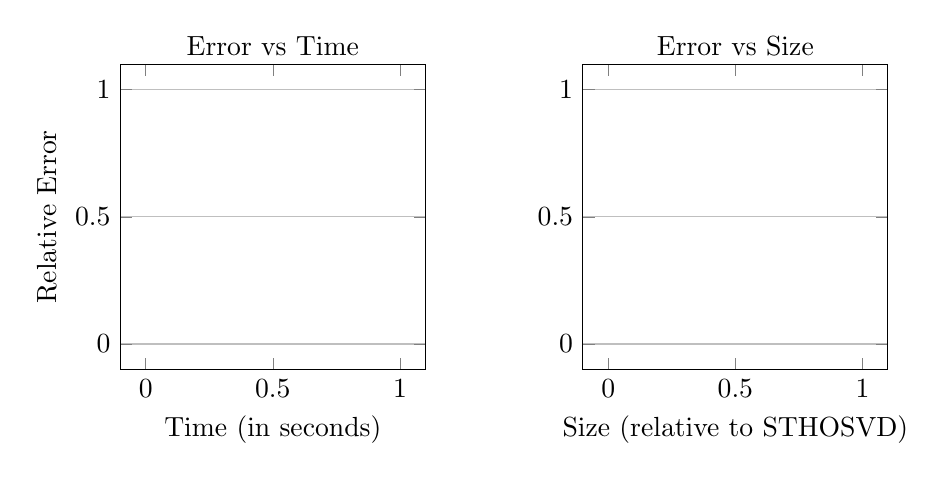
\begin{tikzpicture}
    \begin{groupplot}[
        group style={
            group size=2 by 1,
            xlabels at=edge bottom,
            ylabels at=edge left,
            horizontal sep=2cm,
            vertical sep=2cm,
        },
        width= 0.45\textwidth,
        height=0.45\textwidth,
        ylabel=Relative Error,
        ylabel near ticks,
        xlabel near ticks,
        ymajorgrids=true,
        legend to name=namedlegend,
        legend style={draw=none, cells={anchor=west}, font=\small,
        legend columns=2},
        title style={yshift=-1.5ex},
      ]
        % First plot: error vs time
        \nextgroupplot[
            title=Error vs Time, 
            xlabel=Time (in seconds),
            ytick = \thresh,
            yticklabel style={/pgf/number format/fixed}
        ]

	\foreach \t in \thresh {
		\addplot [HOOIstyle,mark=triangle] table[x=\algorithmname_Time, y=\algorithmname_Error, col sep=comma] {\datapath_\t_Over.csv};
        		\addplot [HOOIstyle,mark=star] table[x=\algorithmname_Time, y=\algorithmname_Error, col sep=comma] {\datapath_\t_Perfect.csv};
        		\addplot [HOOIstyle,mark=square] table[x=\algorithmname_Time, y=\algorithmname_Error, col sep=comma] {\datapath_\t_Under.csv};
        		\addplot [STHOSVDstyle] table[x=STHOSVD_Time, y=STHOSVD_Error, col sep=comma] {\datapath_\t_Under.csv};	
	}
      
        % Second plot: error vs relative size
        \nextgroupplot[
            title=Error vs Size,
            xlabel=Size (relative to STHOSVD),
            ytick = \thresh,
            yticklabel style={/pgf/number format/fixed}
        ]
        
        \foreach \t in \thresh {
        		\addplot[HOOIstyle,mark=triangle] table [x expr = (\thisrow{HOSI_DT_Size}/\thisrow{STHOSVD_Size}), y=HOSI_DT_Error, col sep=comma] {\datapath_\t_Over.csv};
        		\addplot[HOOIstyle,mark=star] table [x expr = (\thisrow{HOSI_DT_Size}/\thisrow{STHOSVD_Size}), y=HOSI_DT_Error, col sep=comma] {\datapath_\t_Perfect.csv};
        		\addplot[HOOIstyle,mark=square] table [x expr = (\thisrow{HOSI_DT_Size}/\thisrow{STHOSVD_Size}), y=HOSI_DT_Error, col sep=comma] {\datapath_\t_Under.csv};
        		\addplot[STHOSVDstyle] table [x expr = (\thisrow{STHOSVD_Size}/\thisrow{STHOSVD_Size}), y=STHOSVD_Error, col sep=comma] {\datapath_\t_Under.csv};
        }

        \addlegendimage{mark=triangle, color=red}
        \addlegendentry{HOSI-DT Over}
        \addlegendimage{mark=star, color=red}
        \addlegendentry{HOSI-DT Perfect}
        \addlegendimage{mark=square, color=red}
        \addlegendentry{HOSI-DT Under}
        \addlegendimage{mark=square*, color=blue, only marks}
        \addlegendentry{STHOSVD}
    \end{groupplot}
\end{tikzpicture}

% Place the legend below the figure
\begin{center}
    \ref{namedlegend}
\end{center}

 

            \caption[SP Dataset - Progression of Time, Error, and Relative Size]{Progression of time, error, and relative size over 3 iterations of rank-adaptive HOSI-DT on the SP dataset using 2048 cores.}
            \label{fig:SP}
        \end{figure}

        \begin{figure}
            \centering
            \renewcommand{\datapath}{data/SP/N16_n2048}
            \renewcommand{\thresh}{1e-01,5e-02,1e-02}
            %!TEX root = ../../main.tex


\newcommand{\maxiter}{3}
\pgfmathsetmacro{\n}{\maxiter - 1}

\begin{tikzpicture}
    \begin{axis}[
        hide axis, % Hide the dummy axis
        axis lines=none,
        xmin=0, xmax=1,
        ymin=0, ymax=1,
        width= 0.45\textwidth,
        height=0.45\textwidth,
        legend style={fill=white, at={(2.25, -0.515)}, anchor=north east, font=\small},
        legend columns=1, % Arrange legend in one column
        reverse legend
    ]   
        \addplot [color=white, fill=white, mark=square*,opacity=0] coordinates {(0,0)};
        \addlegendentry{}

        \addlegendimage{mark=square*, color=blue!25, fill=blue!25, only marks, mark options={scale=2.5, fill=blue!25}}
        \addlegendentry{TTM Comp}

        \addlegendimage{mark=square*, color=blue!50, fill=blue!50, only marks, mark options={scale=2.5, fill=blue!50}}
        \addlegendentry{TTM Comm}

        \addlegendimage{mark=square*, color=red!25, fill=red!25, only marks, mark options={scale=2.5, fill=red!25}}
        \addlegendentry{Contraction Comp}

        \addlegendimage{mark=square*, color=red!50, fill=red!50, only marks, mark options={scale=2.5, fill=red!50}}
        \addlegendentry{Contraction Comm}

        \addlegendimage{mark=square*, color=yellow!50, fill=yellow!50, only marks, mark options={scale=2.5, fill=yellow!50}}
        \addlegendentry{Eig/QR}

        \addlegendimage{mark=square*, color=green!25, fill=green!25, only marks, mark options={scale=2.5, fill=green!25}}
        \addlegendentry{Core Comp}
        
        \addlegendimage{mark=square*, color=green!50, fill=green!50, only marks, mark options={scale=2.5, fill=green!50}}
        \addlegendentry{Core Comm}
    \end{axis}

    \begin{groupplot}[
        group style={
            group size=2 by 2,
            horizontal sep=2cm,
            vertical sep=2cm,
        },
        ybar stacked,
        symbolic x coords={HOSI-DT-Under, HOSI-DT-Perfect, HOSI-DT-Over, STHOSVD},
        xticklabels={Under, Perfect, Over, STHOSVD},
        xtick=data,
        ylabel={Time},
        ylabel style = {yshift=-.675cm},
        ymajorgrids=true,
        width=0.45\textwidth,
        height=0.45\textwidth,
        x tick label style={rotate=30, anchor=east},
        title style={yshift=-1.5ex},
    ]

    \xintFor #1 in \thresh \do {
        \nextgroupplot[title = {#1 Error}]
        \foreach \i in {0, ..., \n} {    
            \addplot[ybar,color=blue,fill=blue!25] 
            		table[x=Algorithm, y=TTM_Computation_Iter_\i, col sep=comma] {\datapath_#1_Breakdown.csv};  
		
            \addplot[ybar,color=blue,fill=blue!50] 
            		table[x=Algorithm, y=TTM_Communication_Iter_\i, col sep=comma] {\datapath_#1_Breakdown.csv};
		
            \addplot[ybar,color=red,fill=red!25] 
            		table[x=Algorithm, y=GramLQ_Computation_Iter_\i, col sep=comma] {\datapath_#1_Breakdown.csv};
		
            \addplot[ybar,color=red,fill=red!50] 
    		table[x=Algorithm, y=GramLQ_Communication_Iter_\i, col sep=comma] {\datapath_#1_Breakdown.csv};
		
            \addplot[ybar,color=yellow,fill=yellow!50] 
    		table[x=Algorithm, y=EigSVD_Iter_\i, col sep=comma] {\datapath_#1_Breakdown.csv};
		
            \addplot[ybar,color=green,fill=green!25] 
    		table[x=Algorithm, y=Core_Analysis_Iter_\i, col sep=comma] {\datapath_#1_Breakdown.csv};
		
            \addplot[ybar,color=green,fill=green!50] 
    		table[x=Algorithm, y=Core_Gathering_Iter_\i, col sep=comma] {\datapath_#1_Breakdown.csv};
        }
    }

\end{groupplot}
\end{tikzpicture}

            \caption[SP Dataset - Running Time Breakdown]{Running time breakdown for the SP dataset using 2048 cores under different levels of compression.}
            \label{fig:SP_breakdown}
        \end{figure}



        \newpage





    %%%%%%%%%%%%%%%%
    %% References %%
    %%%%%%%%%%%%%%%%
    \addcontentsline{toc}{chapter}{\textbf{REFERENCES}}
    \printbibliography
    




    %%%%%%%%
    %% CV %%
    %%%%%%%%
    \addcontentsline{toc}{chapter}{\textbf{CURRICULUM VITAE}}

\end{document}
